\documentclass[10pt]{article}

%=========================== Packages ===========================
\usepackage[a4paper, tmargin=0.75in, lmargin=0.80in, rmargin=0.80in, bmargin=1in]{geometry}
\usepackage{graphicx}
\usepackage{float}
\usepackage{caption}
\usepackage{hyperref}
\usepackage{amssymb}
\usepackage{amsmath}
\usepackage{cite}
\usepackage{enumitem}
\pagestyle{plain}

\setcounter{secnumdepth}{4}
\setcounter{tocdepth}{4}
\makeatletter
\renewcommand\paragraph{\@startsection{paragraph}{4}{\z@}%
    {3.25ex \@plus1ex \@minus.2ex}%
    {1.5ex \@plus.2ex}%
    {\normalfont\normalsize\bfseries}}
\makeatother

%=========================== Custom Information ===========================
\newcommand{\studentname}{Muhammad Zharfan Wiranata}
\newcommand{\studentnumber}{12345678}
\newcommand{\researchcentre}{RF \& Microwave Lab, NSYSU, Taiwan}
\newcommand{\projecttitle}{Basic FMCW Radar}
\newcommand{\supervisor}{Dr A. N. Other}

%=========================== Document Starts Here ===========================
\begin{document}
\pagenumbering{arabic}

%=========================== Title Page ===========================
\begin{center}
    {\Huge\bfseries Weekly Research Report} \\[2mm]
    % {\Large\textbf{ROC-Driven Design of Liquid Crystal MIMO Phased Array Radar: Physical Parameter Optimization under Channel and Noise Constraints}}\\
    % {\large (or customize with your real title)}\\
\end{center}

\vspace{4mm}
\hrule
\vspace{1mm}
\hrule

\vspace{3mm}
\begin{tabular}{ll}
    \textbf{Name}              & \studentname \\
    \textbf{Research Centre}   & \researchcentre \\
    % \textbf{Project Title}     & \projecttitle \\
    % \textbf{Supervisor}        & \supervisor \\
    % \textbf{Week}              & \#xx (e.g., Week 5) \\
    \textbf{Date}              & \today \\
\end{tabular}

\vspace{3mm}
\hrule
\vspace{1mm}
\hrule

%=========================== Sections ===========================
\section{Objectives This Week}
% Jelaskan tujuan utama minggu ini
\begin{itemize}
    \item Evaluate the antenna lens response for a 3TX-to-1RX configuration using the ray-tracing method in Sionna RT.
\end{itemize}

\section{Simulation Antenna Lens Variance Incident of 3TX to 3RX with SIONNA-RT}
This Simulation is conducted using the SIONNA-RT ray-tracing method to evaluate the antenna lens response for a 3TX-to-1RX configuration. This simulation is used to equal setup simulation with HFSS SBR+, but features in SIONNA RT does not support variance of Antenna Radiation Pattern in single simulation. To fulfill the simulation requirement, the simulation is conducted in three separate simulations, each with a different RX antenna radiation pattern. Then the simulation results are combined to evaluate the channel response for the 3TX-to-3RX configuration for configure MIMO Simulation.

Detail of Theory on Sionna RT is attached in the Appendix Section. 
\subsection{Experimental Setup}
As written above, that Experiment setup is used to equal HFSS SBR+. The simulation was conducted in an isolated indoor environment with room dimensions of 3meter x 5meter x 3meter. The room walls were modeled as concrete with a thickness of 0.2 meter. RX Antenna With Lens Enhanced on the center of the room with Operating Frequency of 38GHz. Full detail of the simulation setup is shown in the figure below. 

\begin{figure}[H]
    \centering
    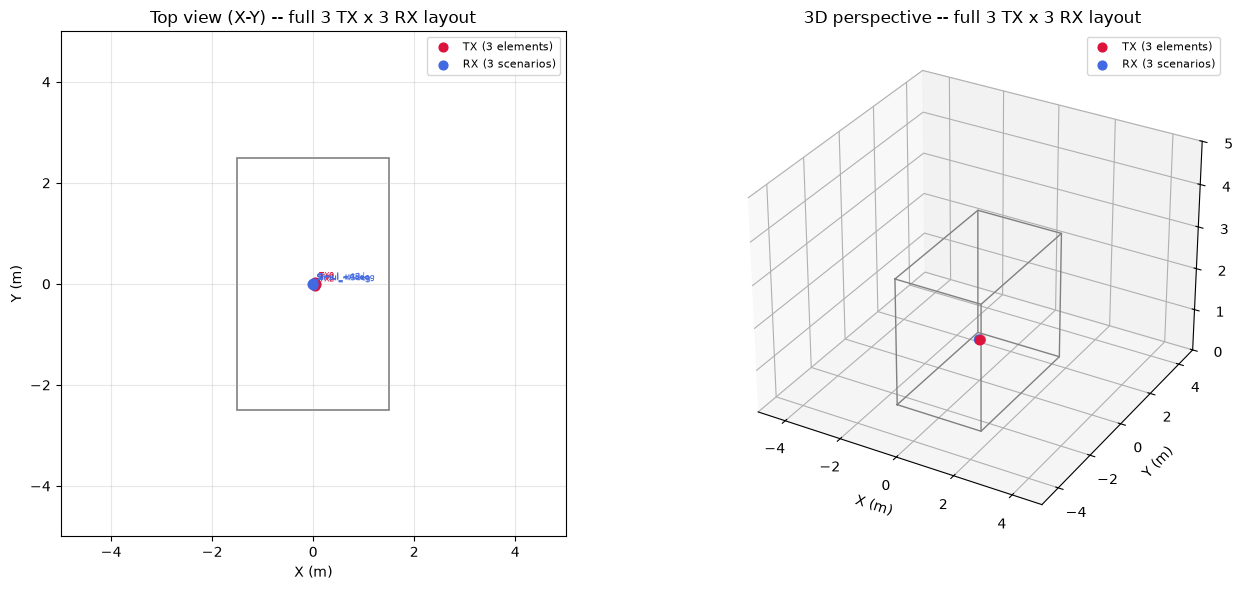
\includegraphics[width=0.85\textwidth]{image/SionnaSim_TotalView.png}
    \caption{Overall indoor simulation environment used for the Sionna-RT experimental setup, showing the room geometry and antenna-lens placement.}
    \label{fig:sionna_total_view}
\end{figure}

\begin{figure}[H]
    \centering
    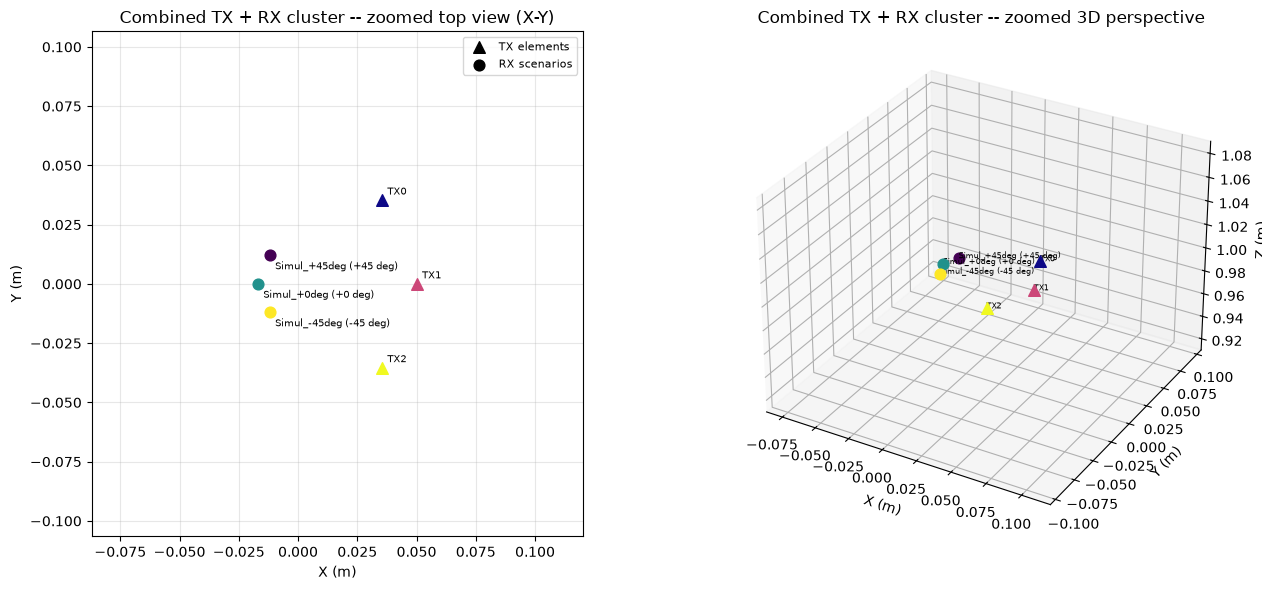
\includegraphics[width=0.85\textwidth]{image/SionnaSim_ZoomView.png}
    \caption{Zoomed view of the Sionna-RT experimental setup highlighting the antenna-lens position at the center of the room and the detailed observation region.}
    \label{fig:sionna_zoom_view}
\end{figure}

\subsection{Result}

The channel generated by Sionna-RT follows a multipath frequency- and
impulse-response formulation. For a frequency $f$, the channel frequency
response is defined as the ratio between the received voltage $V_{\mathrm{R}}$
and the voltage $V_{\mathrm{T}}$ applied to the transmitting antenna,
\begin{equation}
    H(f)
    = \frac{V_{\mathrm{R}}}{V_{\mathrm{T}}}
    = \frac{V_{\mathrm{R}}}{\lvert V_{\mathrm{T}}\rvert},
    \label{eq:sionna_channel_frequency_response}
\end{equation}
where the input voltage is assumed to have zero phase. Sionna-RT determines a
set of $N$ propagation paths between each TX--RX pair. For path $i$, the total
path length $r_i$ and average propagation speed $c_i$ define the propagation
delay $\tau_i=r_i/c_i$. The corresponding complex path coefficient
$\alpha_i$ includes the effects of free-space spreading, material
interactions, polarization, and the transmitting and receiving antenna
patterns. The resulting channel frequency response can therefore be written as
\begin{equation}
    H(f) = \sum_{i=1}^{N} \alpha_i e^{-j2\pi f\tau_i}.
    \label{eq:sionna_multipath_frequency_response}
\end{equation}
This expression is consistent with the electromagnetic channel construction
used by Sionna-RT~\cite{NVIDIACorporation2026} and with the standard tapped-delay
line representation of a multipath wireless channel~\cite{Tse2005}.

Applying the inverse Fourier transform to
(\ref{eq:sionna_multipath_frequency_response}) gives the passband channel
impulse response
\begin{equation}
    h(\tau)
    = \sum_{i=1}^{N}\alpha_i\delta(\tau-\tau_i).
    \label{eq:sionna_passband_impulse_response}
\end{equation}
With the carrier frequency $f_{\mathrm{c}}$, the equivalent complex-baseband
channel is
\begin{equation}
    h_{\mathrm{b}}(\tau)
    = \sum_{i=1}^{N}
      \underbrace{\alpha_i e^{-j2\pi f_{\mathrm{c}}\tau_i}}_
      {\alpha_i^{\mathrm{b}}}
      \delta(\tau-\tau_i),
    \label{eq:sionna_baseband_impulse_response}
\end{equation}
where $\alpha_i^{\mathrm{b}}$ is the complex baseband coefficient of path $i$.
Thus, the Sionna-RT result is a coherent sum of all resolved propagation paths:
their amplitudes and phases determine $H(f)$, while their delays determine the
locations of the impulses in $h_{\mathrm{b}}(\tau)$. Consequently,
constructive and destructive interference among the paths produces the
frequency-selective channel observed in the following results.

The Sionna-RT simulation was evaluated as a wideband channel centered at
$f_{\mathrm{c}}=38~\mathrm{GHz}$ with a total bandwidth of
$B=2~\mathrm{GHz}$. Therefore, the channel response was observed over the
frequency range from $37~\mathrm{GHz}$ to $39~\mathrm{GHz}$. This range was
uniformly sampled using $N_f=401$ frequency points, including both band
edges, which corresponds to a frequency spacing of
\[
    \Delta f=\frac{B}{N_f-1}
    =\frac{2~\mathrm{GHz}}{400}
    =5~\mathrm{MHz}.
\]
For each TX--RX link, Sionna-RT first determines the propagation paths in
the indoor environment, including their delay, attenuation, phase, and
interaction with the surrounding objects. These path parameters are then
used to calculate the complex channel frequency response at every sampled
frequency. Consequently, the resulting data describe both the magnitude
and phase variation of the channel across the complete $2~\mathrm{GHz}$
band, rather than only the response at the center frequency. The same
frequency grid is used in the three simulations with different RX antenna
radiation patterns, allowing their channel responses to be combined
consistently into the equivalent $3\times3$ MIMO channel matrix.

The magnitude plotted for every TX--RX link is obtained from its complex
frequency response using
\begin{equation}
    H_{\mathrm{dB}}(f)=20\log_{10}\left|H(f)\right|.
    \label{eq:sionna_channel_magnitude_db}
\end{equation}
Thus, a less-negative value represents a stronger received channel, and the
lens contribution for the same link can be expressed as
\begin{equation}
    \Delta H_{\mathrm{lens}}(f)
    =H_{\mathrm{with~lens,dB}}(f)
    -H_{\mathrm{without~lens,dB}}(f).
    \label{eq:sionna_lens_channel_gain}
\end{equation}

\begin{figure}[H]
    \centering
    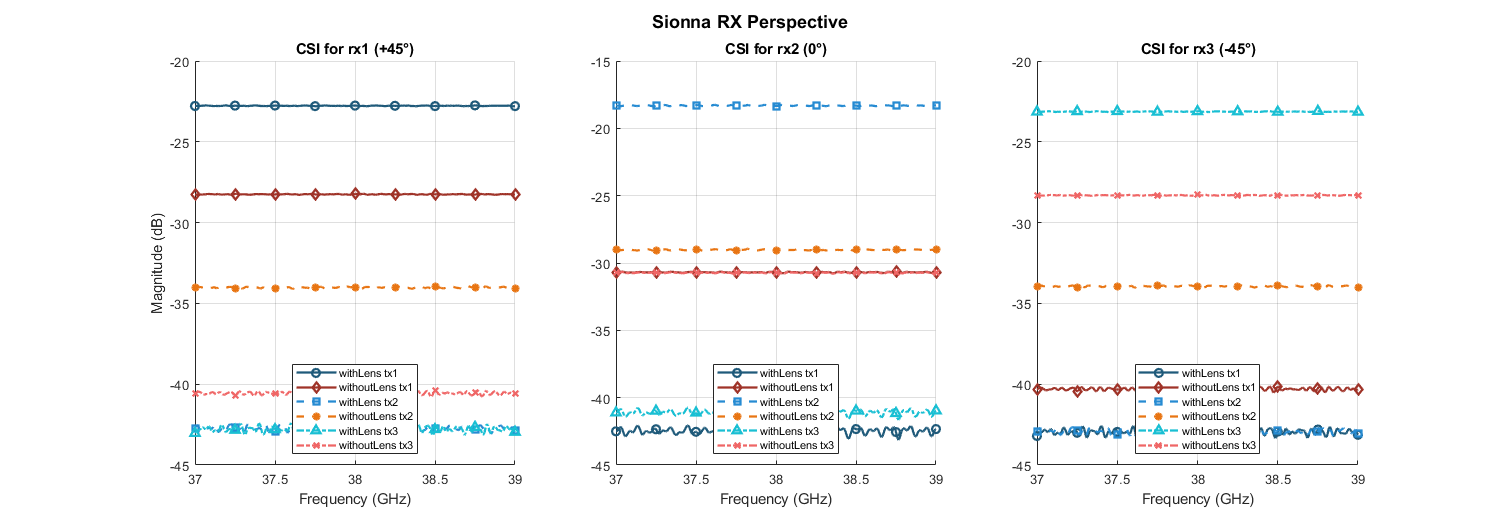
\includegraphics[width=\textwidth]{image/Sionna_result.png}
    \caption{Magnitude of the Sionna-RT channel frequency response from
    37--39~GHz for the three RX perspectives, comparing the with-lens and
    without-lens cases for TX1, TX2, and TX3. The intended angularly aligned
    links are TX1--RX1 at $+45^\circ$, TX2--RX2 at $0^\circ$, and TX3--RX3 at
    $-45^\circ$.}
    \label{fig:sionna_channel_magnitude}
\end{figure}

Figure~\ref{fig:sionna_channel_magnitude} shows that the lens strengthens the
channel associated with the angularly aligned TX--RX pair. Approximate values
read from the curves are summarized in Table~\ref{tab:sionna_aligned_link_gain}.
Because the curves are nearly flat over 37--39~GHz, their representative
levels and the resulting lens gains remain almost constant across the analyzed
band.

\begin{table}[H]
    \centering
    \caption{Approximate channel magnitude and lens gain for the angularly
    aligned TX--RX links in Fig.~\ref{fig:sionna_channel_magnitude}.}
    \label{tab:sionna_aligned_link_gain}
    \begin{tabular}{lccc}
        \hline
        \textbf{Aligned link} &
        \textbf{With lens (dB)} &
        \textbf{Without lens (dB)} &
        \textbf{$\Delta H_{\mathrm{lens}}$ (dB)} \\
        \hline
        TX1--RX1 ($+45^\circ$) & $-22.7$ & $-28.3$ & $+5.6$ \\
        TX2--RX2 ($0^\circ$)   & $-18.2$ & $-29.0$ & $+10.8$ \\
        TX3--RX3 ($-45^\circ$) & $-23.0$ & $-28.3$ & $+5.3$ \\
        \hline
    \end{tabular}
\end{table}

The strongest response is obtained for TX2--RX2, where the lens increases the
channel magnitude by approximately $10.8$~dB. The two oblique aligned links,
TX1--RX1 and TX3--RX3, improve by approximately $5.6$~dB and $5.3$~dB,
respectively. In contrast, several non-aligned links become weaker. In the
RX2 perspective, for example, the with-lens TX1 and TX3 responses are near
$-42$ to $-41$~dB, whereas their without-lens responses are near $-30.5$~dB.
This indicates that the lens not only increases the desired directional
coupling but also suppresses energy arriving from non-matched angular
directions.

In conclusion, the Sionna-RT magnitude results demonstrate angular channel
selectivity: each RX obtains its strongest lens-assisted response from the TX
whose direction is aligned with that RX. The stable response across the
$2$~GHz bandwidth further indicates that this focusing behavior is broadband
over the simulated range. Therefore, the lens improves separation between the
dominant entries of the $3\times3$ channel matrix, although it does not provide
uniform gain to every TX--RX link.

\subsection{Evaluation}

Following the channel formulation and magnitude analysis presented above, the
Sionna-RT results are evaluated from a MIMO communication perspective. At each
sampled frequency, the complex channel responses of all TX--RX pairs are
assembled into a $3\times3$ channel matrix, preserving both the amplitude and
phase information produced by the ray-tracing simulation. This representation
allows the individual propagation links to be assessed jointly as a spatial
communication channel rather than as independent received-power curves.

The evaluation focuses on how the antenna lens changes the strength,
frequency stability, and spatial separation of the channel coefficients. The
with-lens and without-lens cases are compared under the same propagation
geometry so that any observed difference can be attributed to the lens. The
subsequent MIMO metrics are then used to determine whether the directional
focusing observed in Fig.~\ref{fig:sionna_channel_magnitude} produces a more
useful channel matrix for separating the three transmitted signals.

The numerical SVD, condition-number, effective-rank, and 20-dB capacity values
reported in this evaluation are calculated from the 802 records in
\texttt{sionna\_mimo\_summary.csv}, comprising 401 frequency samples for each
of the with-lens and without-lens datasets. Capacity at the other SNR values is
recomputed from the three singular values using
(\ref{eq:sionna_mimo_capacity}). The coupling-gain and spatial-correlation
values are read from their corresponding simulation figures because those
metrics are not included in the summary CSV.

\subsubsection{Lens-Induced Change in TX--RX Coupling}

Before evaluating the matrix-level metrics, the lens-induced change of each
channel coefficient is calculated using
(\ref{eq:sionna_lens_channel_gain}). Figure~\ref{fig:sionna_lens_effect_delta}
shows that the lens selectively enhances the angularly matched links while
attenuating most cross-directional links.

\begin{figure}[H]
    \centering
    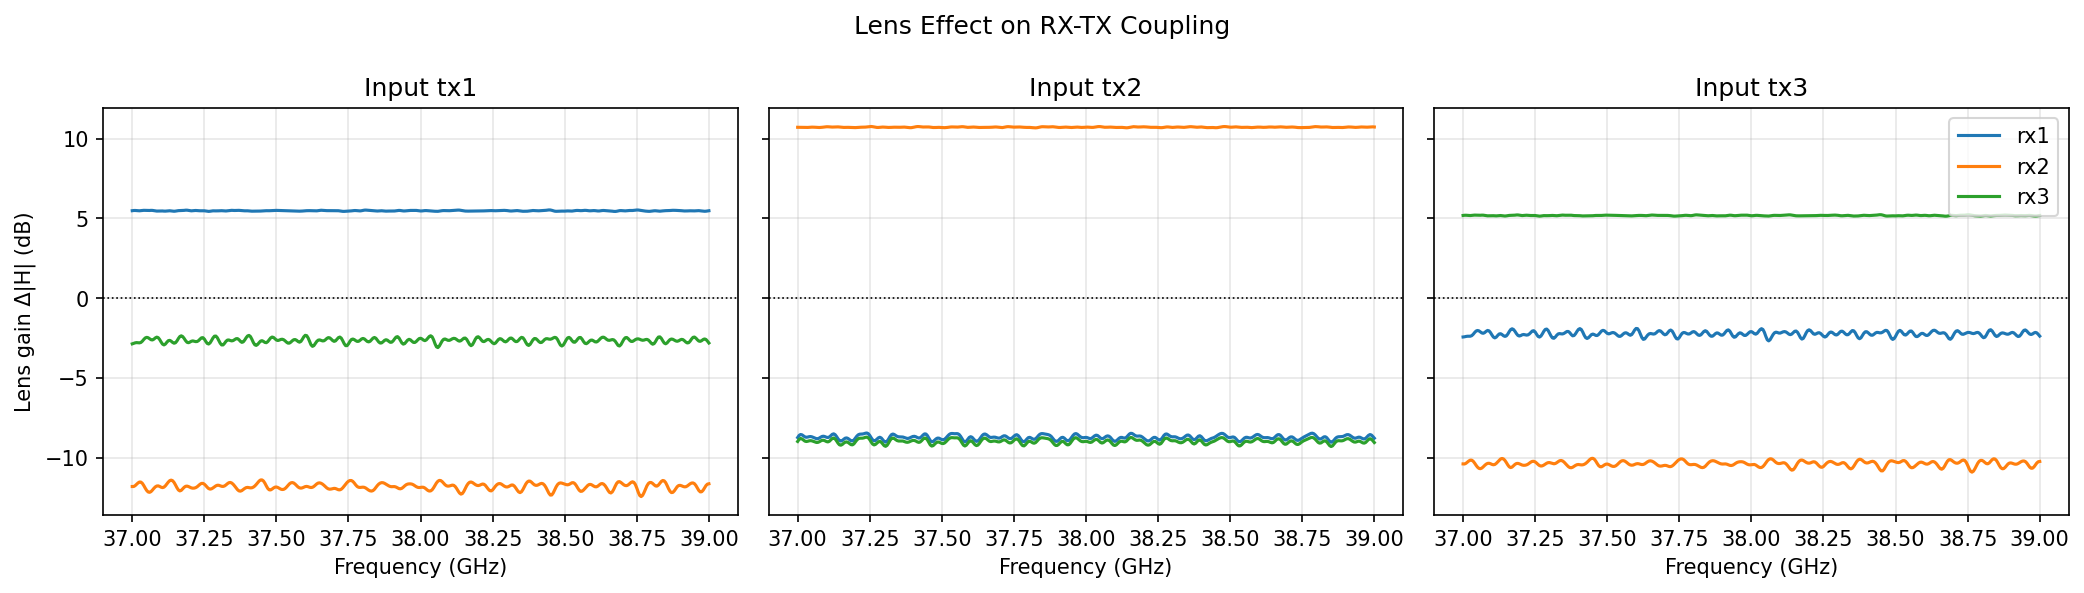
\includegraphics[width=\textwidth]{image/sionna_lens_effect_delta.png}
    \caption{Lens-induced change in the Sionna-RT channel magnitude for every
    TX--RX pair. Positive values indicate enhancement and negative values
    indicate attenuation relative to the without-lens case.}
    \label{fig:sionna_lens_effect_delta}
\end{figure}

The intended TX1--RX1, TX2--RX2, and TX3--RX3 links obtain approximately
$+5.5$~dB, $+10.7$~dB, and $+5.1$~dB of gain, respectively. Conversely, the
non-aligned links are reduced by approximately $2.5$--$12$~dB. These changes
are almost constant across 37--39~GHz. The lens therefore reshapes the channel
matrix toward stronger direction-matched coefficients and weaker
cross-coupling, rather than applying a uniform gain to all entries.

\subsubsection{Singular-Value Decomposition and Channel Quality}

For each frequency, the channel matrix is decomposed as
\begin{equation}
    \mathbf{H}(f)
    =\mathbf{U}(f)\boldsymbol{\Sigma}(f)\mathbf{V}^{H}(f),
    \qquad
    \boldsymbol{\Sigma}(f)
    =\operatorname{diag}\{\sigma_1,\sigma_2,\sigma_3\},
    \label{eq:sionna_svd}
\end{equation}
where $\sigma_1\geq\sigma_2\geq\sigma_3$ are the singular values. The condition
number and effective rank are used to describe the balance and number of
usable spatial modes:
\begin{equation}
    \kappa(f)=\frac{\sigma_1(f)}{\sigma_3(f)},
    \qquad
    r_{\mathrm{eff}}(f)
    =\exp\left(-\sum_{i=1}^{3}p_i(f)\ln p_i(f)\right),
    \quad
    p_i(f)=\frac{\sigma_i(f)}{\sum_{k=1}^{3}\sigma_k(f)}.
    \label{eq:sionna_channel_quality}
\end{equation}
A condition number closer to one indicates more balanced singular modes,
whereas an effective rank closer to three indicates that more independent
spatial modes contribute to the channel.

\begin{figure}[H]
    \centering
    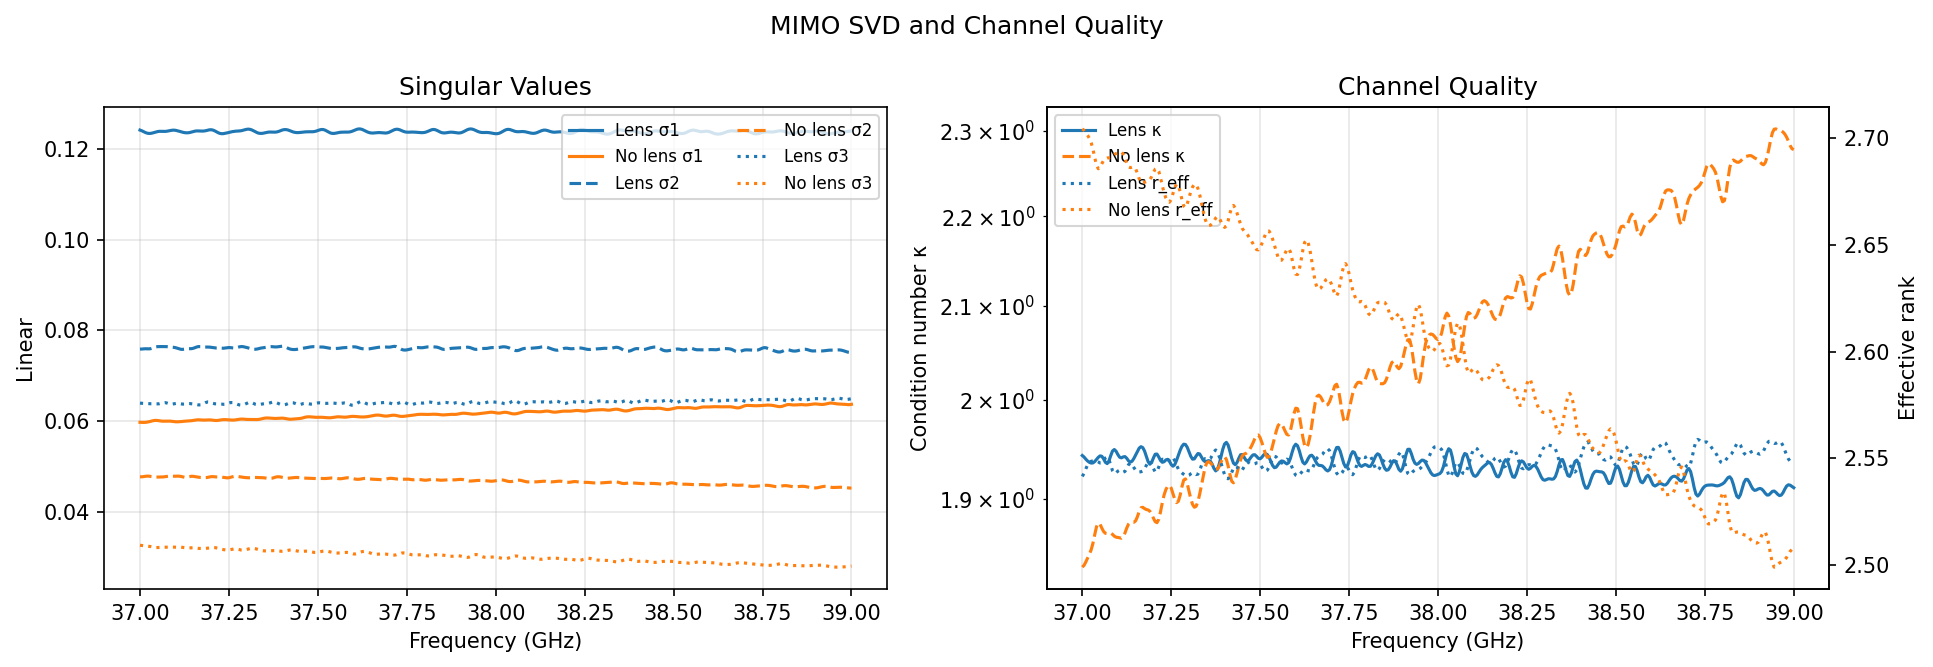
\includegraphics[width=\textwidth]{image/sionna_mimo_quality.png}
    \caption{Singular values, condition number, and effective rank of the
    Sionna-RT $3\times3$ MIMO channel with and without the antenna lens over
    37--39~GHz.}
    \label{fig:sionna_mimo_quality}
\end{figure}

As shown in Fig.~\ref{fig:sionna_mimo_quality}, the mean with-lens singular
values are $\sigma_1=0.1239$, $\sigma_2=0.0760$, and $\sigma_3=0.0642$.
Their full-band ranges are $0.1233$--$0.1245$, $0.0751$--$0.0765$, and
$0.0635$--$0.0650$, respectively. Without the lens, the corresponding means
are $0.0618$, $0.0467$, and $0.0300$, with ranges of
$0.0597$--$0.0640$, $0.0452$--$0.0478$, and $0.0277$--$0.0326$. Thus, the
lens increases not only the dominant mode but also the second and third
modes, which is important for supporting multiple spatial streams.

The with-lens condition number spans $1.901$--$1.957$, with a mean of
$1.931$. Without the lens, it spans $1.834$--$2.302$, with a mean of
$2.066$; its value specifically increases from $1.834$ at 37~GHz to $2.278$
at 39~GHz. The lens therefore provides more stable conditioning across the
band, although the without-lens channel has the lower condition number near
37~GHz. The effective-rank result also requires a qualified interpretation:
the with-lens mean is $2.549$, whereas the without-lens mean is slightly
higher at $2.603$. The without-lens effective rank, however, decreases from
$2.704$ at 37~GHz to $2.507$ at 39~GHz, while the with-lens value remains in
the narrow range $2.541$--$2.559$. Therefore, the principal lens benefit is
the larger and more frequency-stable singular-mode strength; it is not a
uniform increase in effective rank at every frequency.

\subsubsection{MIMO Channel Capacity}

Assuming equal power allocation across the three transmitters and spatially
white receiver noise, the MIMO capacity is evaluated as
\begin{equation}
    C(f,\rho)
    =\log_2\det\left(
      \mathbf{I}_{3}
      +\frac{\rho}{3}\mathbf{H}(f)\mathbf{H}^{H}(f)
    \right)
    \quad \text{bps/Hz},
    \label{eq:sionna_mimo_capacity}
\end{equation}
where $\rho$ is the linear SNR. This calculation includes the contribution of
all three singular modes.

\begin{figure}[H]
    \centering
    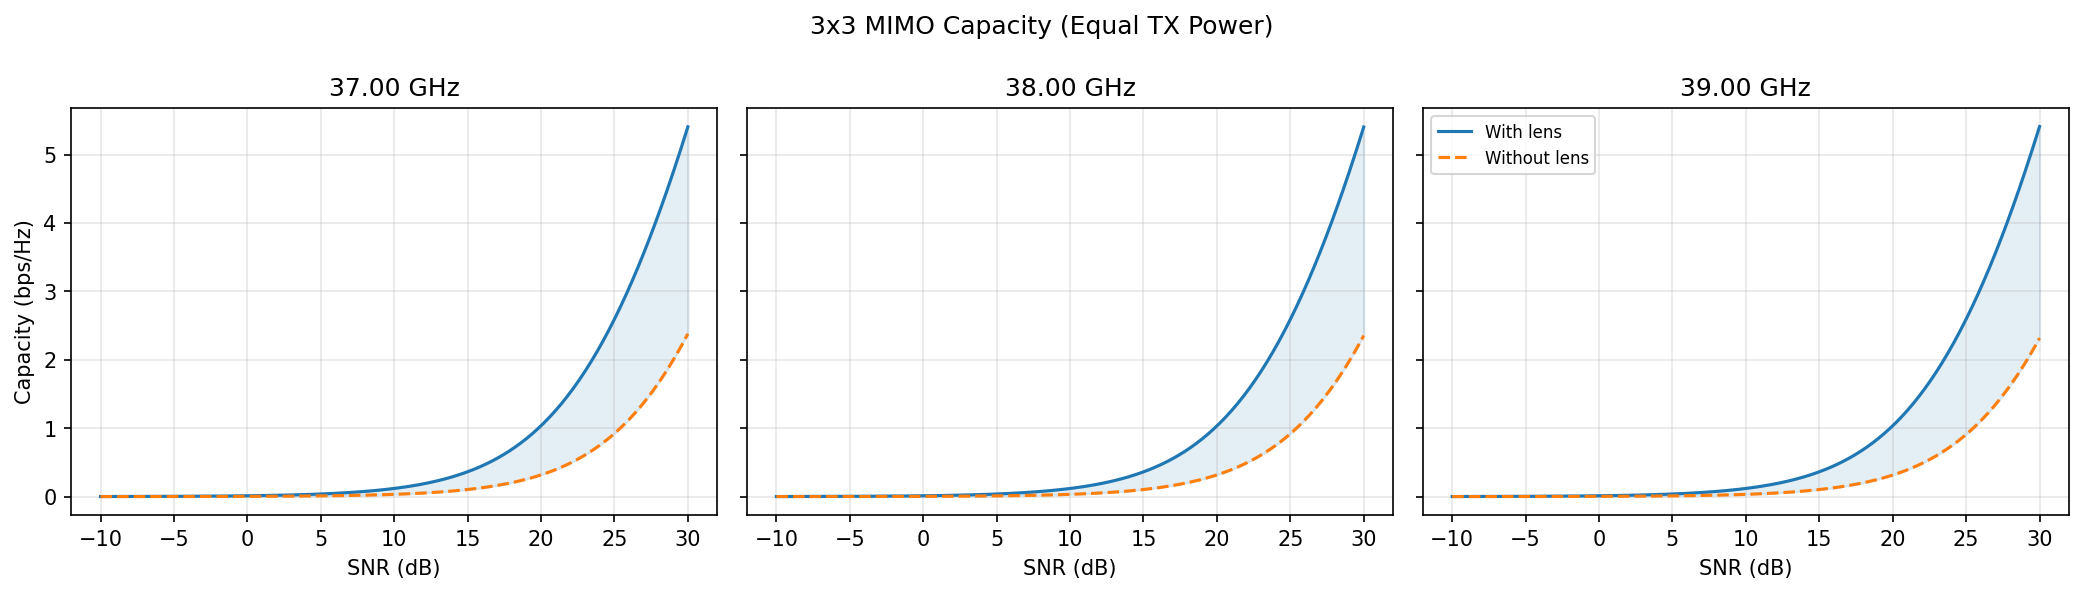
\includegraphics[width=\textwidth]{image/sionna_mimo_capacity.png}
    \caption{Equal-transmit-power $3\times3$ MIMO capacity versus SNR at
    37, 38, and 39~GHz for the Sionna-RT channels with and without the
    antenna lens.}
    \label{fig:sionna_mimo_capacity}
\end{figure}

Figure~\ref{fig:sionna_mimo_capacity} shows a consistent capacity advantage
for the lens-assisted channel at all three evaluated frequencies. At
30~dB SNR, the full-band mean capacity is $5.406$~bps/Hz with the lens and
$2.351$~bps/Hz without the lens. Their respective full-band ranges are
$5.385$--$5.425$~bps/Hz and $2.314$--$2.381$~bps/Hz. The small difference
among the 37, 38, and 39~GHz panels confirms that the capacity benefit is
maintained across the simulated bandwidth.

\begin{figure}[H]
    \centering
    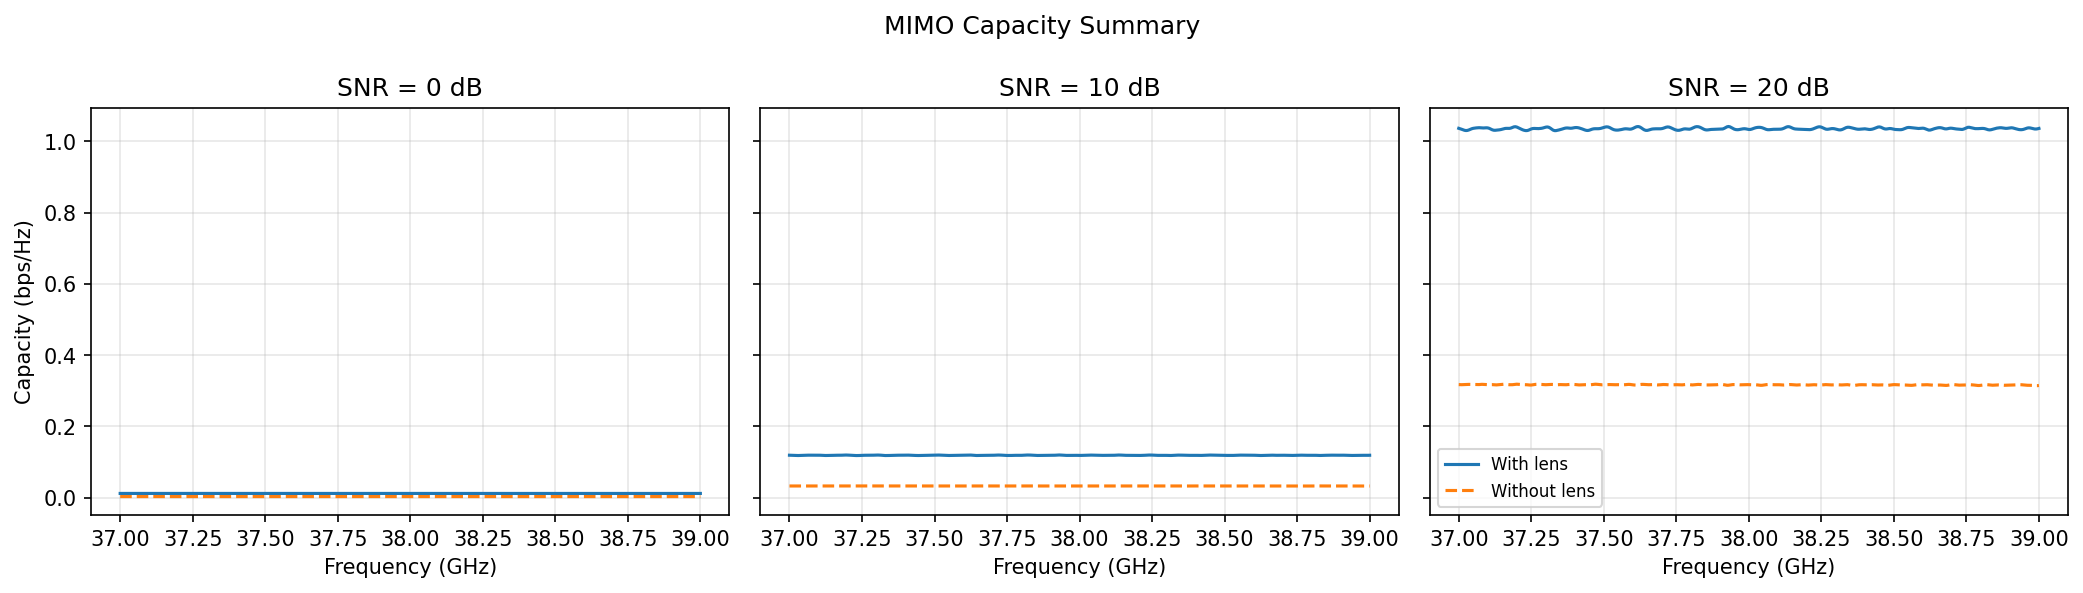
\includegraphics[width=\textwidth]{image/sionna_mimo_capacity_summary.png}
    \caption{Frequency-domain summary of the Sionna-RT MIMO capacity at
    SNR values of 0, 10, and 20~dB, comparing the with-lens and without-lens
    channels.}
    \label{fig:sionna_mimo_capacity_summary}
\end{figure}

The frequency-domain summary in
Fig.~\ref{fig:sionna_mimo_capacity_summary} further shows that the capacity is
nearly frequency-flat. The full-band mean capacities at 0~dB are $0.01211$
and $0.00332$~bps/Hz for the with-lens and without-lens channels,
respectively. At 10~dB, the means are $0.1191$ and $0.03303$~bps/Hz. At
20~dB, they increase to $1.0353$ and $0.3169$~bps/Hz. Therefore, the
capacity ratios in favor of the lens are approximately $3.65$, $3.61$, and
$3.27$ at 0, 10, and 20~dB, respectively, under the normalization used in
this simulation.

\subsubsection{Spatial Correlation}

The normalized correlation matrices at the receiver and transmitter sides are
calculated from
\begin{equation}
    \mathbf{R}_{\mathrm{RX}}
    =\mathbf{D}_{\mathrm{RX}}^{-1/2}
      \mathbf{H}\mathbf{H}^{H}
      \mathbf{D}_{\mathrm{RX}}^{-1/2},
    \qquad
    \mathbf{R}_{\mathrm{TX}}
    =\mathbf{D}_{\mathrm{TX}}^{-1/2}
      \mathbf{H}^{H}\mathbf{H}
      \mathbf{D}_{\mathrm{TX}}^{-1/2},
    \label{eq:sionna_spatial_correlation}
\end{equation}
where $\mathbf{D}_{\mathrm{RX}}$ and $\mathbf{D}_{\mathrm{TX}}$ contain the
corresponding diagonal power terms. Smaller off-diagonal magnitudes indicate
better spatial separation.

\begin{figure}[H]
    \centering
    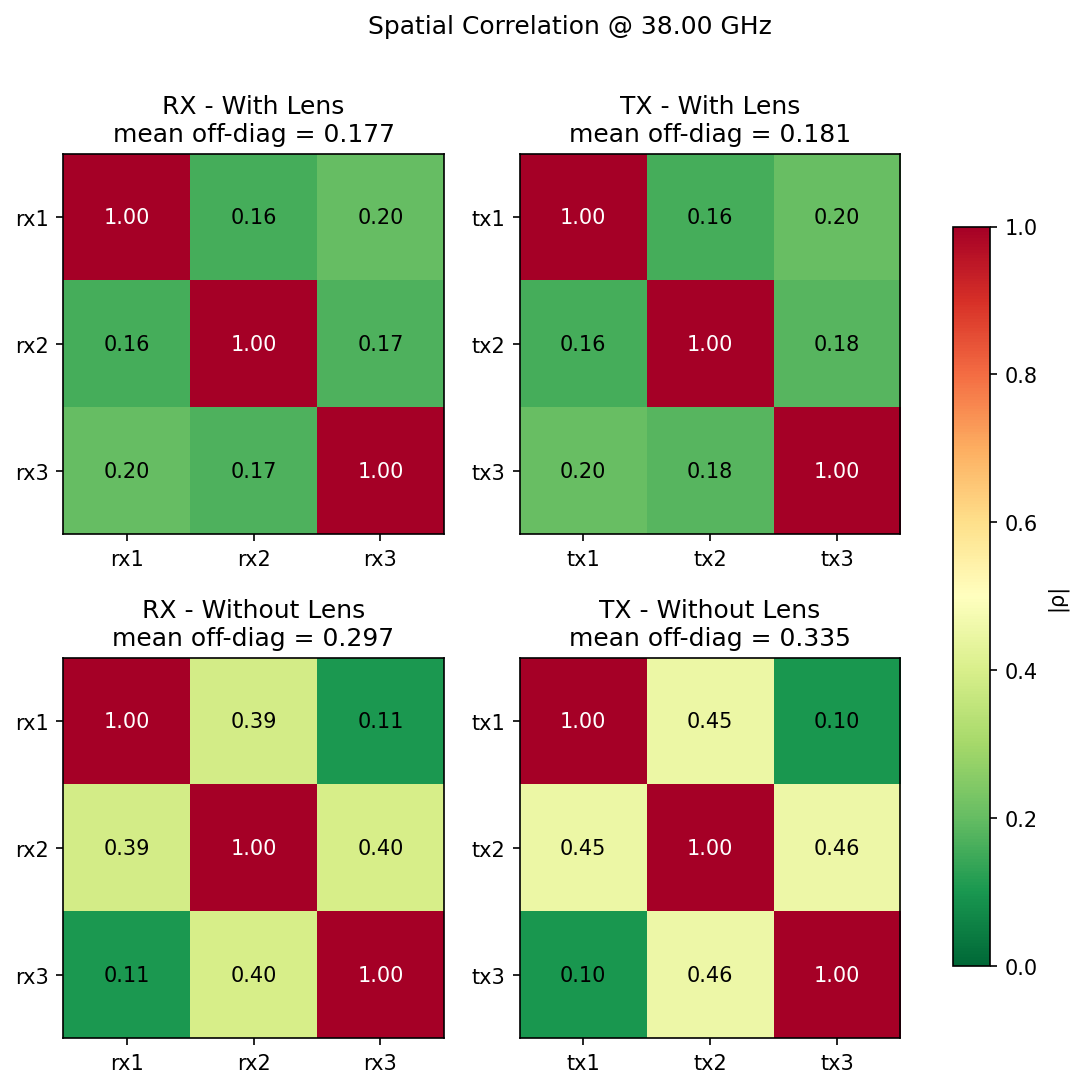
\includegraphics[width=0.82\textwidth]{image/sionna_spatial_correlation.png}
    \caption{Normalized RX- and TX-side spatial-correlation magnitudes at
    38~GHz for the Sionna-RT channels with and without the antenna lens.}
    \label{fig:sionna_spatial_correlation}
\end{figure}

At 38~GHz, the mean off-diagonal RX correlation decreases from $0.297$
without the lens to $0.177$ with the lens, corresponding to a reduction of
approximately $40.4\%$. The mean TX correlation similarly decreases from
$0.335$ to $0.181$, a reduction of approximately $46.0\%$. With the lens, all
displayed off-diagonal coefficients lie between $0.16$ and $0.20$. Without
the lens, several coefficients involving the central channel reach
$0.39$--$0.46$. The lens therefore produces more weakly correlated TX and RX
channel vectors.

Overall, the Sionna-RT evaluation shows that the antenna lens improves the
MIMO channel in complementary ways: it strengthens all three singular modes,
maintains stable channel conditioning, increases equal-power capacity, and
reduces spatial correlation. These results support the conclusion that the
directional focusing observed in the individual channel magnitudes translates
into a stronger and more separable $3\times3$ MIMO channel. The effective-rank
data nevertheless show that this improvement should be attributed primarily
to stronger and more stable eigenchannels, rather than to a higher effective
rank throughout the entire frequency band.


\section{Simulation Antenna Lens Variance Incident of 1TX to 3RX with Hybrid Method on HFSS Hybrid Solver}

\subsection{Experimental Setup}
\begin{figure}[H]
    \centering
    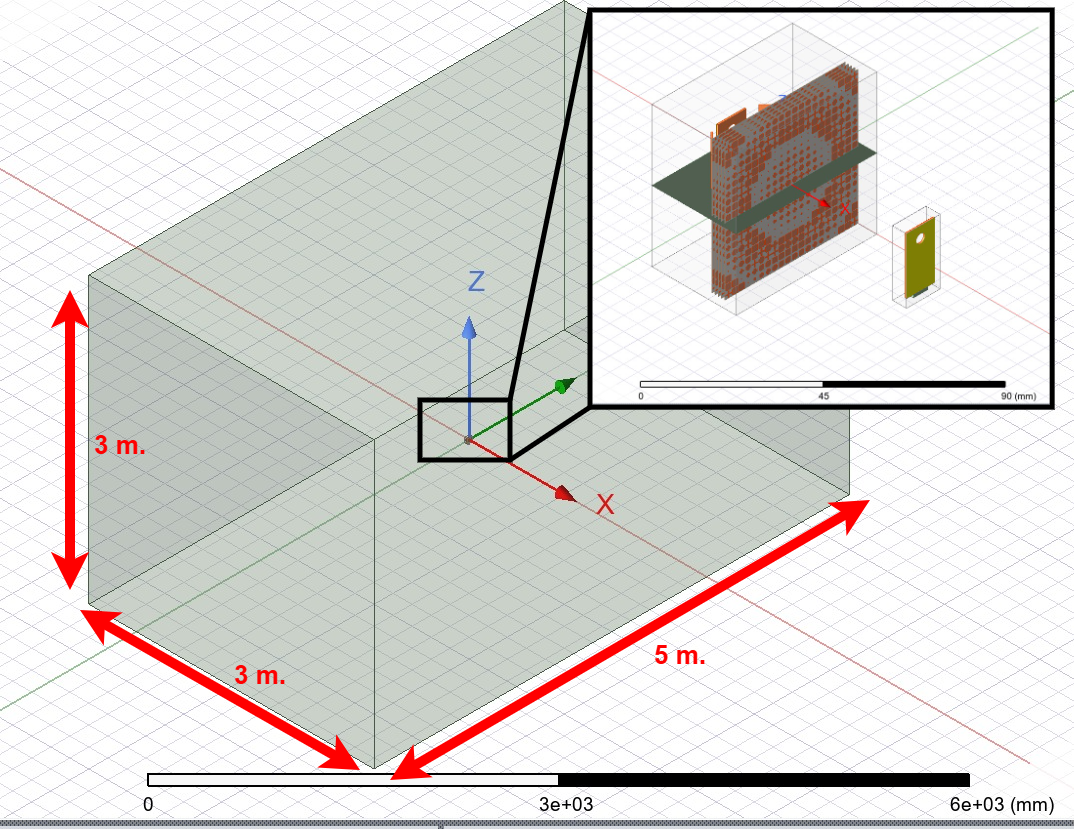
\includegraphics[width=0.85\textwidth]{image/Room_withCloseup.png}
    \caption{Indoor simulation room and close-up view of the antenna lens placement.}
\end{figure}

    The simulation was conducted in an isolated indoor environment with room dimensions of
    $3~\mathrm{m} \times 5~\mathrm{m} \times 3~\mathrm{m}$. The room walls were modeled as concrete
    with a thickness of $0.2~\mathrm{m}$. The antenna lens was placed near the center of the room,
    with dimensions of $0.5~\mathrm{m} \times 0.5~\mathrm{m} \times 0.01~\mathrm{m}$. The operating
    frequency was set to 38 GHz. The lens was designed to focus the incoming signal at a distance of
    1 m from the lens surface, corresponding to the intended focal length.

    To evaluate the channel improvement introduced by the antenna lens, the simulation was performed
    using the same room geometry and identical TX/RX positions for two cases: with the antenna lens
    and without the antenna lens. This configuration ensures that the comparison is based only on the
    presence of the lens, while the propagation environment and antenna locations remain unchanged.

    In this setup, one swept TX source and three RX observation points were used. The RX points were
    placed behind the lens along the focal radius, with RX1 at $0^\circ$, RX2 at $+45^\circ$, and
    RX3 at $-45^\circ$. For naming consistency, the swept TX2 source is referred to as the
    \textit{incident angle}. TX2 was swept from $+45^\circ$ to $-45^\circ$ with a step size of
    $-45^\circ$ to evaluate how the lens response changes as the incoming direction varies. The
    detailed geometry and placement are shown in the simulation setup figure.

\begin{table}[H]
    \centering
    \caption{Incident-angle simulation configuration for the 1TX-to-3RX setup.}
    \begin{tabular}{lll}
        \hline
        \textbf{Element} & \textbf{Angular Position / Sweep} & \textbf{Description} \\
        \hline
        RX1 & $0^\circ$ & Receiver at the central focal direction \\
        RX2 & $+45^\circ$ & Receiver at the positive-angle focal direction \\
        RX3 & $-45^\circ$ & Receiver at the negative-angle focal direction \\
        TX2 & $+45^\circ$ to $-45^\circ$, step $-45^\circ$ & Swept source, defined as the incident angle \\
        \hline
    \end{tabular}
\end{table}

\begin{figure}[H]
    \centering
    \begin{minipage}{0.32\textwidth}
        \centering
        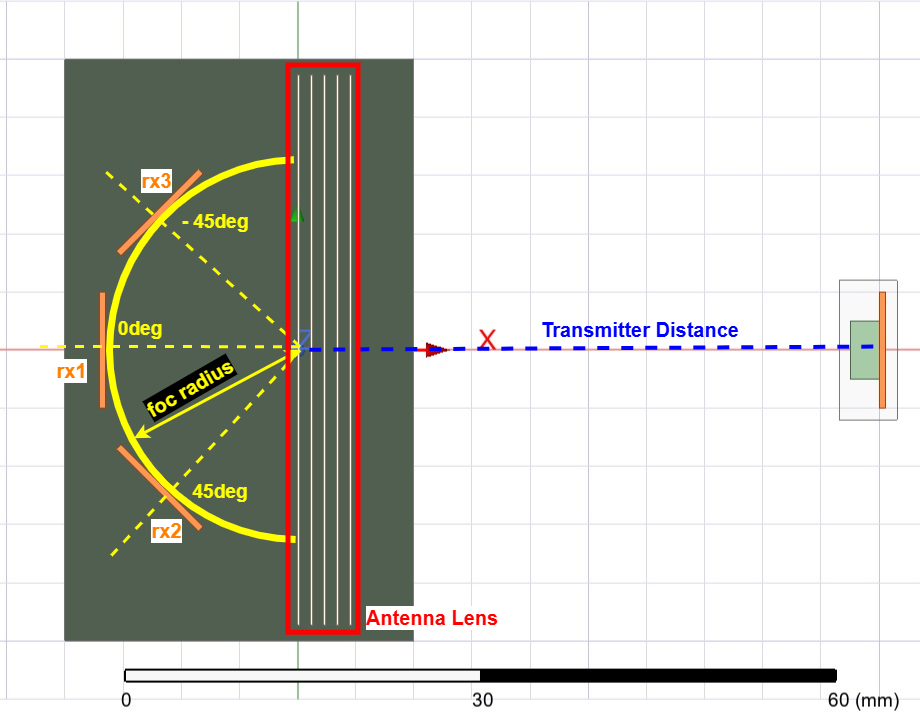
\includegraphics[width=\textwidth]{image/SetupEnvironment_0deg.png}
        \caption*{(a) Incident angle $0^\circ$}
    \end{minipage}
    \hfill
    \begin{minipage}{0.32\textwidth}
        \centering
        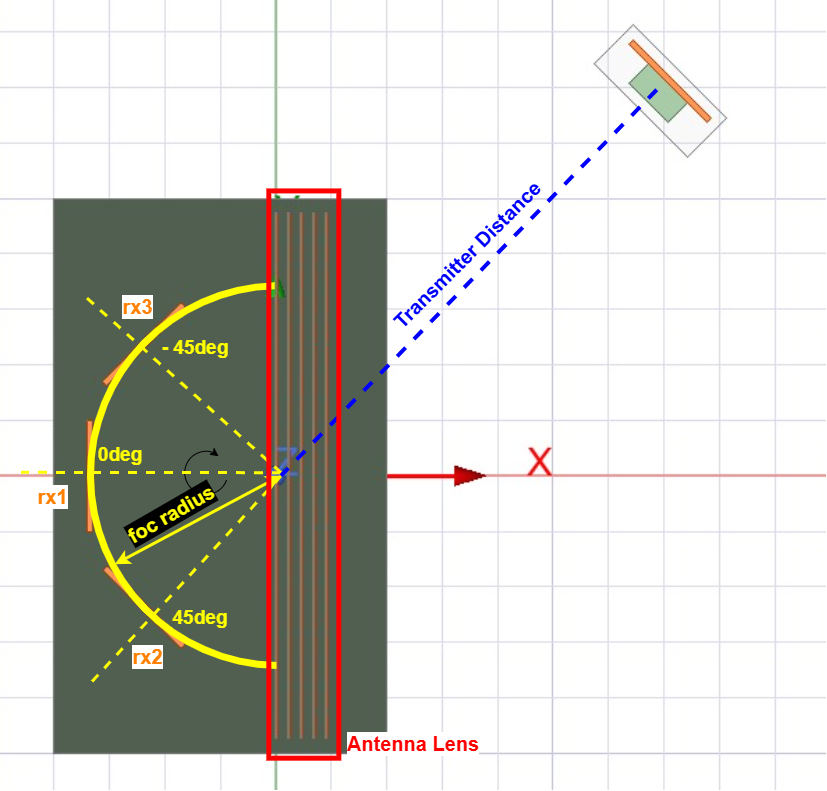
\includegraphics[width=\textwidth]{image/SetupEnvironment_45deg.png}
        \caption*{(b) Incident angle $+45^\circ$}
    \end{minipage}
    \hfill
    \begin{minipage}{0.32\textwidth}
        \centering
        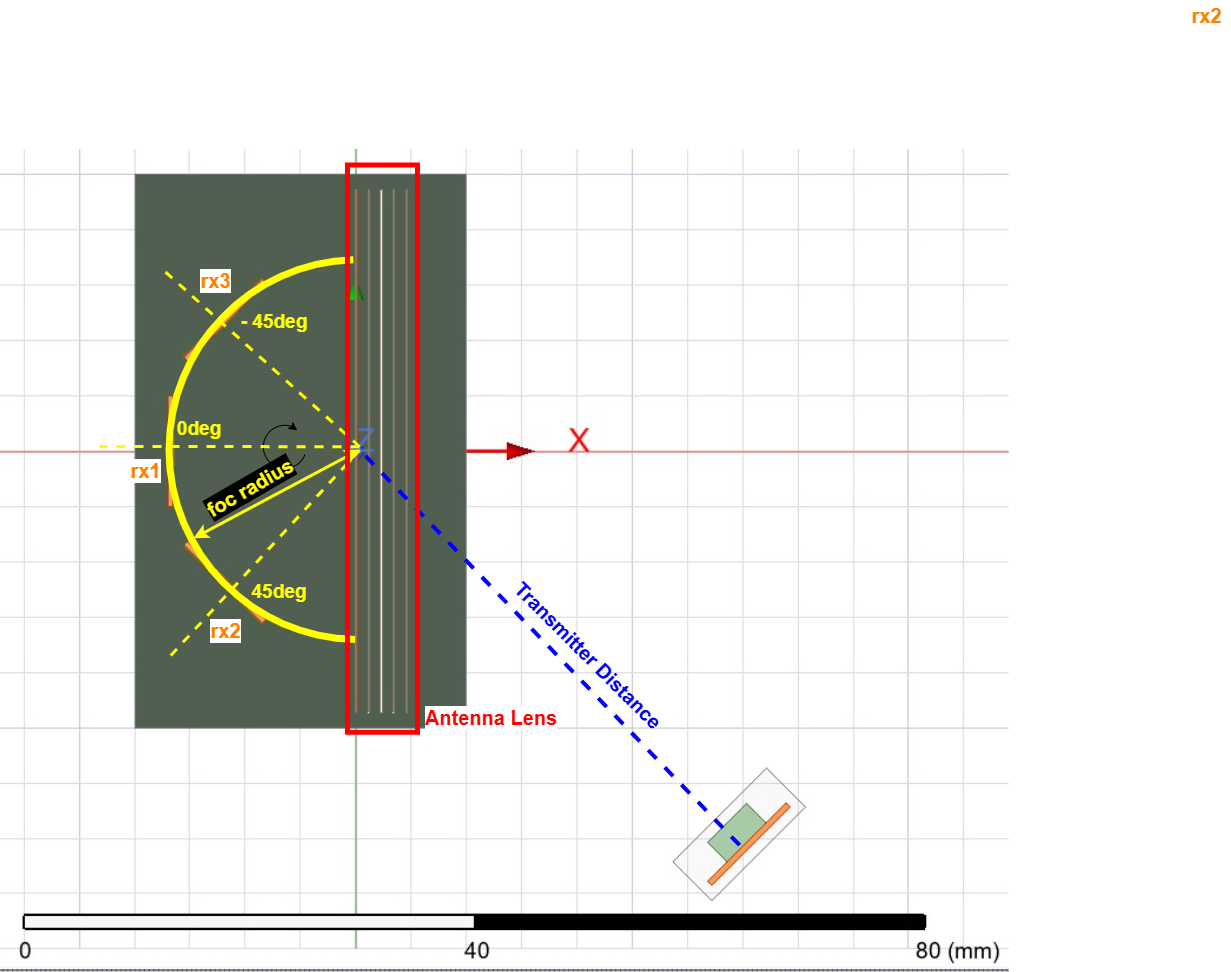
\includegraphics[width=\textwidth]{image/SetupEnvironment_m45deg.png}
        \caption*{(c) Incident angle $-45^\circ$}
    \end{minipage}
    \caption{Simulation environment for the 1TX-to-3RX antenna lens setup under different incident-angle conditions.}
\end{figure}

Overall, six simulations were performed: three incident-angle configurations with the antenna lens
and the same three configurations without the antenna lens. The detailed simulation matrix is
summarized in Table~\ref{tab:hybrid_simulation_matrix}.

\begin{table}[H]
    \centering
    \caption{Hybrid Solver simulation matrix for channel-response evaluation.}
    \label{tab:hybrid_simulation_matrix}
    \footnotesize
    \setlength{\tabcolsep}{5pt}
    \resizebox{\textwidth}{!}{%
    \begin{tabular}{llll}
        \hline
        \textbf{Incident Angle} & \textbf{Simulation Cases} & \textbf{Frequency Sweep} & \textbf{Channel Outputs} \\
        \hline
        $0^\circ$ & With lens and without lens & 36--40 GHz, 1 GHz step & $S_{\mathrm{rx1},\mathrm{tx2}}^{0^\circ}$, $S_{\mathrm{rx2},\mathrm{tx2}}^{0^\circ}$, $S_{\mathrm{rx3},\mathrm{tx2}}^{0^\circ}$ \\
        $+45^\circ$ & With lens and without lens & 36--40 GHz, 1 GHz step & $S_{\mathrm{rx1},\mathrm{tx2}}^{+45^\circ}$, $S_{\mathrm{rx2},\mathrm{tx2}}^{+45^\circ}$, $S_{\mathrm{rx3},\mathrm{tx2}}^{+45^\circ}$ \\
        $-45^\circ$ & With lens and without lens & 36--40 GHz, 1 GHz step & $S_{\mathrm{rx1},\mathrm{tx2}}^{-45^\circ}$, $S_{\mathrm{rx2},\mathrm{tx2}}^{-45^\circ}$, $S_{\mathrm{rx3},\mathrm{tx2}}^{-45^\circ}$ \\
        \hline
    \end{tabular}
    }
\end{table}

% \begin{itemize}
%     \item One TX source and three RX observation points were configured to evaluate the lens response under different incident directions.
%     \item The HFSS Hybrid Solver, including the FE-BI solver, was used to provide a more detailed electromagnetic representation of the antenna lens and its surrounding open-region environment.
%     \item The incident direction of the TX source was varied to observe how the antenna lens response changes at each RX point.
% \end{itemize}

\subsection{Result}
In HFSS, the Hybrid Solver analysis was organized as three separate incident-angle simulations.
Each incident-angle case was repeated twice: one simulation with the antenna lens and one simulation
without the antenna lens. The room geometry, TX position, and RX positions were kept identical in
both cases so that the channel comparison only reflects the effect of the antenna lens.

The received channel response was evaluated using the S-parameter magnitude in dB at each RX point.
The frequency sweep was performed from 36 GHz to 40 GHz with a 1 GHz step. To quantify the lens
contribution, the magnitude difference between the with-lens and without-lens cases was calculated as
\[
    \Delta S_\text{lens} = S_\text{with lens} - S_\text{without lens}.
\]
A positive $\Delta S_\text{lens}$ indicates channel improvement caused by the lens, while a negative
value indicates attenuation relative to the without-lens baseline. All cases were evaluated at RX1,
RX2, and RX3.

The simulated field distribution for each incident-angle case is shown in
Fig.~\ref{fig:hybrid_field_incident_results}. These field plots provide a visual reference for how
the antenna lens redirects the incident wave toward different RX observation regions before the
response is quantified using the S-parameter results.

\begin{figure}[H]
    \centering
    \begin{minipage}{0.32\textwidth}
        \centering
        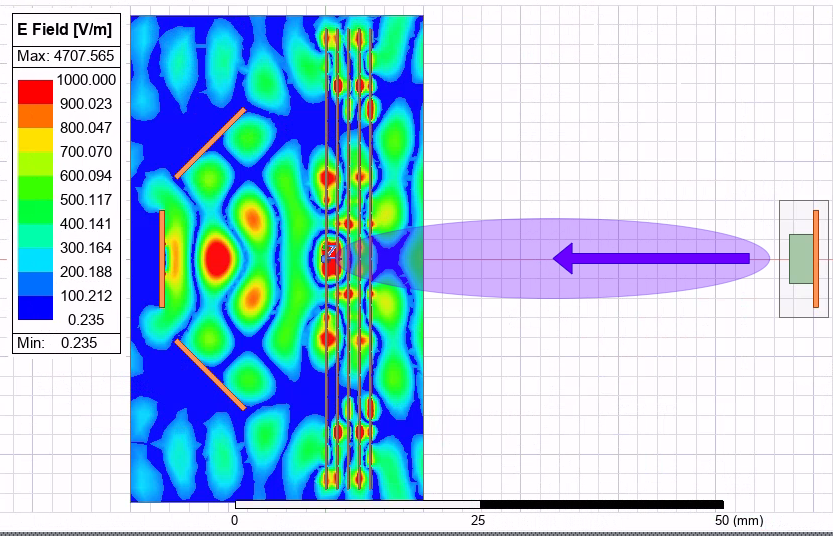
\includegraphics[width=\textwidth]{image/result_field_incident_0deg_edited.PNG}
        \caption*{(a) Incident angle \(0^\circ\)}
    \end{minipage}
    \hfill
    \begin{minipage}{0.32\textwidth}
        \centering
        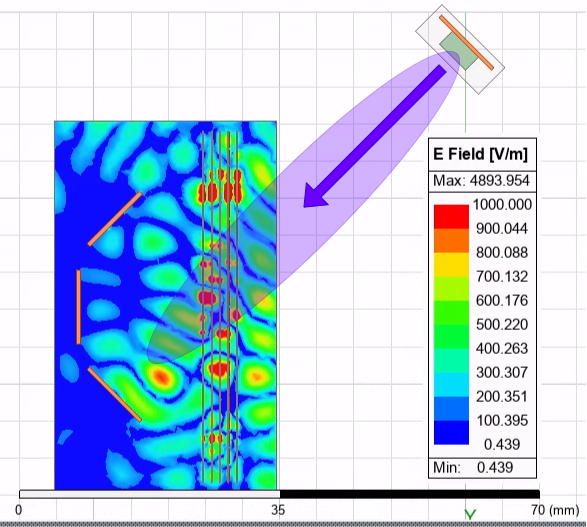
\includegraphics[width=\textwidth]{image/result_field_incident_45deg_edited.PNG}
        \caption*{(b) Incident angle \(+45^\circ\)}
    \end{minipage}
    \hfill
    \begin{minipage}{0.32\textwidth}
        \centering
        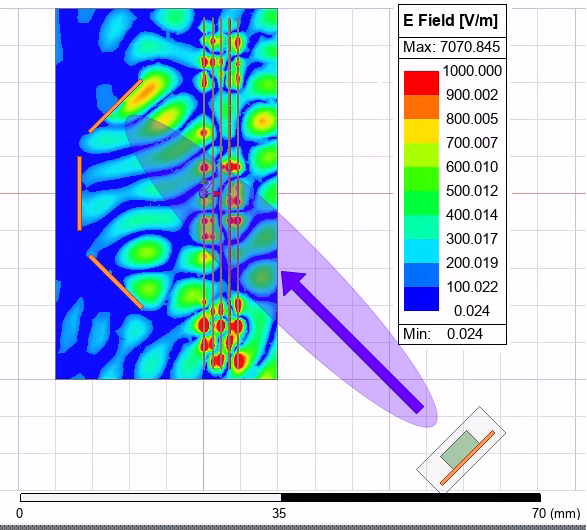
\includegraphics[width=\textwidth]{image/result_field_incident_m45deg_edited.PNG}
        \caption*{(c) Incident angle \(-45^\circ\)}
    \end{minipage}
    \caption{Hybrid Solver field distribution results for the three incident-angle cases.}
    \label{fig:hybrid_field_incident_results}
\end{figure}

Figure~\ref{fig:hybrid_field_incident_results} shows that the received field distribution changes
with the incident direction. The \(0^\circ\) case produces a more central field response, while the
\(+45^\circ\) and \(-45^\circ\) cases shift the dominant field region toward the corresponding
off-axis observation side. This behavior supports the S-parameter evaluation because the received
channel level at each RX depends on how well the lens-directed field aligns with the RX position.

\begin{figure}[H]
    \centering
    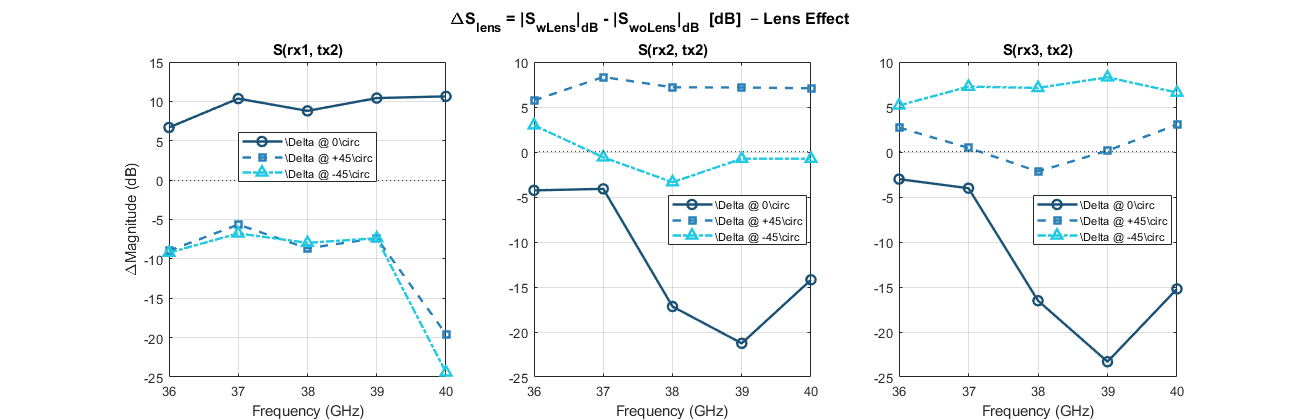
\includegraphics[width=0.85\textwidth]{image/Result_Hybrid_SParam_db_compareLensandNon.png}
    \caption{Comparison of the received channel response with and without the antenna lens using the HFSS Hybrid Solver.}
\end{figure}

\begin{figure}[H]
    \centering
    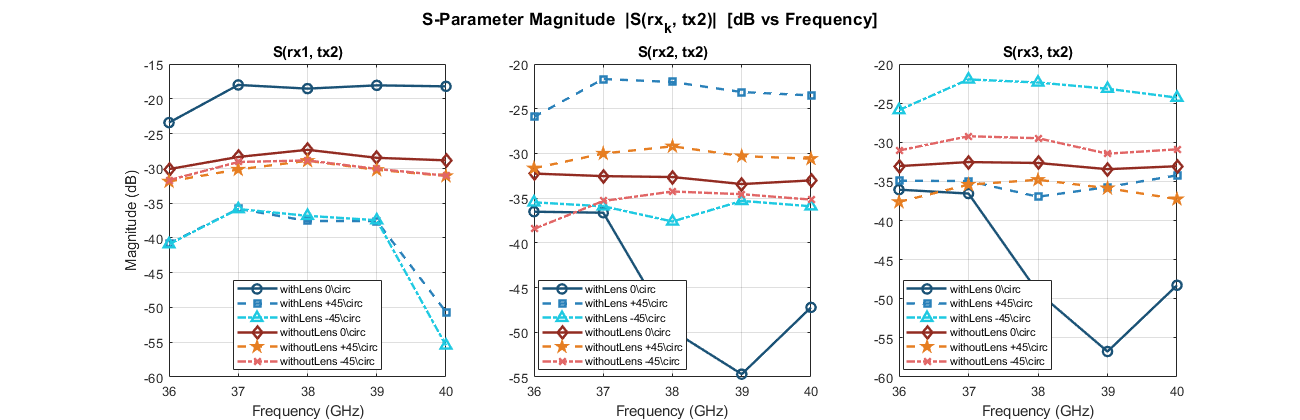
\includegraphics[width=0.85\textwidth]{image/Result_Hybrid_SParam_db.png}
    \caption{S-parameter magnitude response from the HFSS Hybrid Solver incident-angle study.}
\end{figure}

\begin{figure}[H]
    \centering
    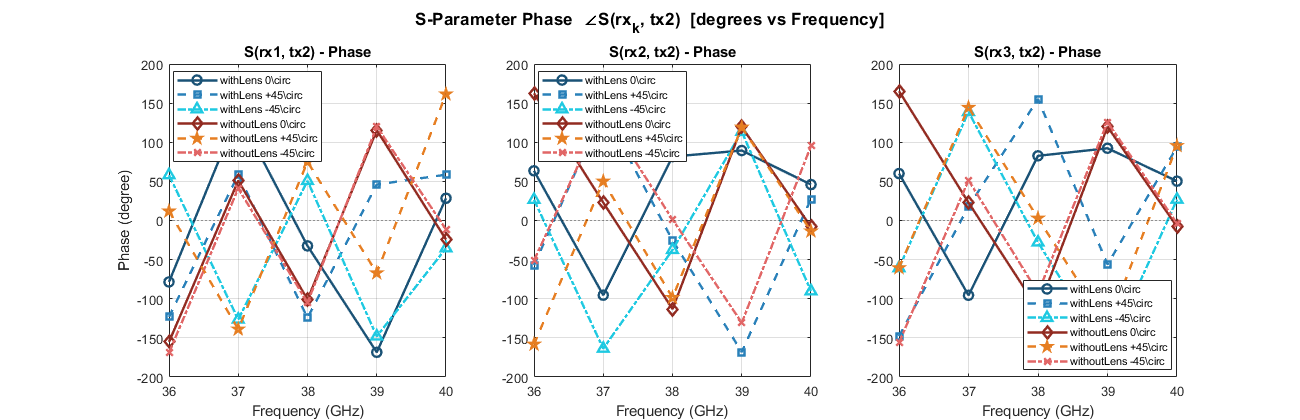
\includegraphics[width=0.85\textwidth]{image/Result_Hybrid_SParam_phase.png}
    \caption{S-parameter phase response from the HFSS Hybrid Solver incident-angle study.}
\end{figure}

The comparison between the with-lens and without-lens cases shows the channel variation introduced by
the antenna lens under the same room and TX/RX placement. The $\Delta S_\text{lens}$ result indicates
strong angular selectivity. For $S_{\mathrm{rx1},\mathrm{tx2}}^{0^\circ}$, the lens provides a gain
improvement of approximately $+2$ to $+11$ dB, while the same lens reduces the received level by up
to approximately $-25$ dB for $S_{\mathrm{rx1},\mathrm{tx2}}^{-45^\circ}$ near 40 GHz.

For $S_{\mathrm{rx2},\mathrm{tx2}}^{+45^\circ}$ and
$S_{\mathrm{rx3},\mathrm{tx2}}^{-45^\circ}$, the improvement is mainly observed at the RX position
aligned with the corresponding incident angle, with an approximate enhancement of $+7$ to $+9$ dB.
In contrast, the $0^\circ$ case shows a notable degradation above 39 GHz for the off-axis RX
positions. This trend indicates that the lens focusing effect is strongly dependent on the alignment
between the incident angle and each RX focal position.

\subsection{Evaluation}

\subsubsection{Angular-Domain Wireless Channel Formulation}

In this work, the received signal at the lens-assisted receiver is formulated using an angular-domain wireless channel model. 
Instead of defining the input vector as signals transmitted from multiple physical transmit antennas, the input is defined as a set of incident angular modes. 
Therefore, the received signal vector can be written as

\begin{equation}
\mathbf{y}(f) = \mathbf{H}_{\theta}(f)\mathbf{x}_{\theta}(f) + \mathbf{n}(f),
\label{eq:angular_channel_model}
\end{equation}

where \(\mathbf{y}(f)\in\mathbb{C}^{N_R \times 1}\) is the received signal vector at the receiver ports, 
\(\mathbf{x}_{\theta}(f)\in\mathbb{C}^{N_{\theta}\times 1}\) is the incident angular excitation vector, 
\(\mathbf{H}_{\theta}(f)\in\mathbb{C}^{N_R \times N_{\theta}}\) is the angular-domain channel matrix, 
and \(\mathbf{n}(f)\in\mathbb{C}^{N_R \times 1}\) represents the additive noise vector.

For the case of three receiving antennas and three incident angles, the received signal vector is expressed as

\begin{equation}
\mathbf{y}(f)=
\begin{bmatrix}
y_1(f)\\
y_2(f)\\
y_3(f)
\end{bmatrix},
\end{equation}

and the incident angular excitation vector is written as

\begin{equation}
\mathbf{x}_{\theta}(f)=
\begin{bmatrix}
x_{\theta_1}(f)\\
x_{\theta_2}(f)\\
x_{\theta_3}(f)
\end{bmatrix},
\end{equation}

where \(x_{\theta_j}(f)\) denotes the incident signal component arriving from the angle \(\theta_j\). 
In this setup, \(\theta_1=0^\circ\), \(\theta_2=+45^\circ\), and \(\theta_3=-45^\circ\).
The corresponding angular-domain channel matrix is given by

\begin{equation}
\mathbf{H}_{\theta}(f)=
\begin{bmatrix}
S_{\mathrm{rx1},\mathrm{tx2}}^{0^\circ}(f) &
S_{\mathrm{rx1},\mathrm{tx2}}^{+45^\circ}(f) &
S_{\mathrm{rx1},\mathrm{tx2}}^{-45^\circ}(f)\\
S_{\mathrm{rx2},\mathrm{tx2}}^{0^\circ}(f) &
S_{\mathrm{rx2},\mathrm{tx2}}^{+45^\circ}(f) &
S_{\mathrm{rx2},\mathrm{tx2}}^{-45^\circ}(f)\\
S_{\mathrm{rx3},\mathrm{tx2}}^{0^\circ}(f) &
S_{\mathrm{rx3},\mathrm{tx2}}^{+45^\circ}(f) &
S_{\mathrm{rx3},\mathrm{tx2}}^{-45^\circ}(f)
\end{bmatrix}.
\label{eq:angular_channel_matrix}
\end{equation}

Thus, the complete input-output relationship can be written as

\begin{equation}
\begin{bmatrix}
y_1(f)\\
y_2(f)\\
y_3(f)
\end{bmatrix}
=
\begin{bmatrix}
S_{\mathrm{rx1},\mathrm{tx2}}^{0^\circ}(f) &
S_{\mathrm{rx1},\mathrm{tx2}}^{+45^\circ}(f) &
S_{\mathrm{rx1},\mathrm{tx2}}^{-45^\circ}(f)\\
S_{\mathrm{rx2},\mathrm{tx2}}^{0^\circ}(f) &
S_{\mathrm{rx2},\mathrm{tx2}}^{+45^\circ}(f) &
S_{\mathrm{rx2},\mathrm{tx2}}^{-45^\circ}(f)\\
S_{\mathrm{rx3},\mathrm{tx2}}^{0^\circ}(f) &
S_{\mathrm{rx3},\mathrm{tx2}}^{+45^\circ}(f) &
S_{\mathrm{rx3},\mathrm{tx2}}^{-45^\circ}(f)
\end{bmatrix}
\begin{bmatrix}
x_{\theta_1}(f)\\
x_{\theta_2}(f)\\
x_{\theta_3}(f)
\end{bmatrix}
+
\begin{bmatrix}
n_1(f)\\
n_2(f)\\
n_3(f)
\end{bmatrix}.
\label{eq:expanded_angular_channel}
\end{equation}

Each coefficient \(S_{\mathrm{rx}i,\mathrm{tx2}}^{\theta_j}(f)\) represents the complex channel response from the incident angular mode \(\theta_j\) to the \(i\)-th receiving antenna. 
For compact notation, this coefficient is defined as

\begin{equation}
h_{i,j}(f) \equiv S_{\mathrm{rx}i,\mathrm{tx2}}^{\theta_j}(f),
\label{eq:s21_channel}
\end{equation}

where \(i\in\{1,2,3\}\) denotes the RX index and \(j\in\{1,2,3\}\) denotes the incident-angle index. 
The measured angle order is \(\theta_1=0^\circ\), \(\theta_2=+45^\circ\), and \(\theta_3=-45^\circ\). 
The complex value of the S-parameter must be used, including both magnitude and phase:

\begin{equation}
S_{\mathrm{rx}i,\mathrm{tx2}}^{\theta_j}(f)
=
\left|S_{\mathrm{rx}i,\mathrm{tx2}}^{\theta_j}(f)\right|
e^{j\angle S_{\mathrm{rx}i,\mathrm{tx2}}^{\theta_j}(f)}.
\label{eq:complex_s21}
\end{equation}

If the VNA data are exported in magnitude in dB and phase in degrees, the complex channel coefficient can be reconstructed as

\begin{equation}
h_{i,j}(f)
=
10^{\frac{S_{\mathrm{rx}i,\mathrm{tx2},\mathrm{dB}}^{\theta_j}(f)}{20}}
e^{j\phi_{i,j}(f)},
\label{eq:s21_db_to_complex}
\end{equation}

where

\begin{equation}
\phi_{i,j}(f)=\frac{\pi}{180}\angle S_{\mathrm{rx}i,\mathrm{tx2}}^{\theta_j}(f).
\end{equation}

During measurement, only one incident angle is excited at a time. 
For example, when the transmitter is placed at the first incidence angle \(\theta_1\), the angular excitation vector becomes

\begin{equation}
\mathbf{x}_{\theta}(f)=
\begin{bmatrix}
1\\
0\\
0
\end{bmatrix}.
\end{equation}

Substituting this into \eqref{eq:angular_channel_model} gives

\begin{equation}
\mathbf{y}_{\theta_1}(f)
=
\mathbf{H}_{\theta}(f)
\begin{bmatrix}
1\\
0\\
0
\end{bmatrix}
+
\mathbf{n}(f)
=
\begin{bmatrix}
S_{\mathrm{rx1},\mathrm{tx2}}^{0^\circ}(f)\\
S_{\mathrm{rx2},\mathrm{tx2}}^{0^\circ}(f)\\
S_{\mathrm{rx3},\mathrm{tx2}}^{0^\circ}(f)
\end{bmatrix}
+
\mathbf{n}(f).
\label{eq:first_column_measurement}
\end{equation}

Therefore, each incidence angle measurement provides one column of the angular-domain channel matrix \(\mathbf{H}_{\theta}(f)\). 
By sequentially placing the transmitting antenna at \(\theta_1\), \(\theta_2\), and \(\theta_3\), all columns of \(\mathbf{H}_{\theta}(f)\) can be measured.

The matrix \(\mathbf{H}_{\theta}(f)\) can therefore be interpreted as the measured angular-domain channel state information (CSI) of the lens-assisted receiver. 
It represents the mapping from incident angular modes to receiver ports. 
However, it should be noted that \(\mathbf{H}_{\theta}(f)\) is not a conventional physical multi-transmitter MIMO channel matrix, because the columns do not correspond to independent physical transmit antennas. 
Instead, each column corresponds to one incident angular excitation state. 
Thus, \(\mathbf{H}_{\theta}(f)\) is more accurately described as an angular-domain CSI matrix, beamspace CSI matrix, or measured effective channel response of the lens-assisted receiver.

\subsubsection{Singular Value Decomposition of the Angular-Domain Channel Matrix}

After the angular-domain channel matrix \(\mathbf{H}_{\theta}(f)\) is constructed from the measured
S-parameters, SVD is used to evaluate how well the antenna lens separates different incident
directions at the receiver ports. In this report, the columns of \(\mathbf{H}_{\theta}(f)\) correspond
to the incident angles \(0^\circ\), \(+45^\circ\), and \(-45^\circ\), while the rows correspond to
RX1, RX2, and RX3. Therefore, the SVD analysis is applied to the measured angular-domain channel
matrix, not to a conventional simultaneous multi-transmitter MIMO channel.

\begin{equation}
\mathbf{H}_{\theta}(f)
=
\mathbf{U}(f)\boldsymbol{\Sigma}(f)\mathbf{V}^{H}(f),
\label{eq:svd_angular_channel}
\end{equation}

where \(\mathbf{U}(f)\) represents the receiver-side modal basis, \(\mathbf{V}(f)\) represents the
incident-angle modal basis, and \(\boldsymbol{\Sigma}(f)\) contains the singular values of the
angular-domain channel matrix:

\begin{equation}
\boldsymbol{\Sigma}(f)
=
\mathrm{diag}
\left(
\sigma_1(f),
\sigma_2(f),
\sigma_3(f)
\right),
\label{eq:svd_sigma}
\end{equation}

with

\begin{equation}
\sigma_1(f)\geq\sigma_2(f)\geq\sigma_3(f)\geq 0.
\label{eq:singular_value_order}
\end{equation}

The singular values quantify the strength of the independent angular response modes supported by
the lens-assisted receiver. If \(\sigma_1(f)\) is much larger than the other singular values, the
measured angular responses are highly correlated and the receiver mainly supports one dominant
effective mode. If \(\sigma_1(f)\), \(\sigma_2(f)\), and \(\sigma_3(f)\) are more balanced, the
incident angular states generate more distinguishable receiver responses, indicating stronger
angular separability.

The condition number is used to evaluate how balanced the angular-domain channel matrix is:

\begin{equation}
\kappa(f)
=
\frac{\sigma_1(f)}{\sigma_3(f)}.
\label{eq:condition_number}
\end{equation}

A lower condition number indicates a more balanced channel matrix. Ideally, \(\kappa(f)\) approaches
unity when all singular values are equal. A high condition number indicates that the measured
angular responses are dominated by one mode and that the channel matrix is poorly conditioned.

The effective rank is also calculated to estimate the number of significant angular modes:

\begin{equation}
p_i(f)
=
\frac{\sigma_i^2(f)}{\sum_{k=1}^{3}\sigma_k^2(f)},
\label{eq:singular_value_probability}
\end{equation}

\begin{equation}
r_{\mathrm{eff}}(f)
=
\exp
\left(
-\sum_{i=1}^{3}
p_i(f)\ln p_i(f)
\right).
\label{eq:effective_rank}
\end{equation}

The effective rank satisfies

\begin{equation}
1 \leq r_{\mathrm{eff}}(f) \leq 3.
\label{eq:effective_rank_range}
\end{equation}

When \(r_{\mathrm{eff}}(f)\) is close to 1, the channel is dominated by a single angular mode. When
\(r_{\mathrm{eff}}(f)\) approaches 3, the three angular response modes are more balanced, indicating
better angular diversity and lower correlation among the measured incident-angle states.

The SVD evaluation results of the constructed \(3\times3\) angular-domain channel matrix
\(\mathbf{H}_{\theta}(f)\) are summarized in Table~\ref{tab:svd_results}. The evaluation compares
the with-lens and without-lens cases across the 36--40 GHz frequency range.

\begin{table}[H]
    \centering
    \caption{SVD evaluation of the \(3\times3\) angular-domain channel matrix \(\mathbf{H}_{\theta}(f)\).}
    \label{tab:svd_results}
    \footnotesize
    \setlength{\tabcolsep}{4pt}
    \resizebox{\textwidth}{!}{%
    \begin{tabular}{lrrrrrr}
        \hline
        \textbf{Condition} & \textbf{Freq. (GHz)} & \(\boldsymbol{\sigma_1}\) & \(\boldsymbol{\sigma_2}\) & \(\boldsymbol{\sigma_3}\) & \(\boldsymbol{\kappa}\) & \(\boldsymbol{r_{\mathrm{eff}}}\) \\
        \hline
        withLens    & 36 & 0.0748 & 0.0667 & 0.0297 & 2.517 & 2.4891 \\
        withLens    & 37 & 0.1308 & 0.0957 & 0.0648 & 2.017 & 2.6084 \\
        withLens    & 38 & 0.1211 & 0.0796 & 0.0767 & 1.579 & 2.7279 \\
        withLens    & 39 & 0.1271 & 0.0847 & 0.0537 & 2.368 & 2.4489 \\
        withLens    & 40 & 0.1232 & 0.0802 & 0.0481 & 2.560 & 2.3817 \\
        \hline
        withoutLens & 36 & 0.0591 & 0.0387 & 0.0136 & 4.337 & 2.1033 \\
        withoutLens & 37 & 0.0723 & 0.0455 & 0.0160 & 4.517 & 2.0630 \\
        withoutLens & 38 & 0.0772 & 0.0479 & 0.0174 & 4.424 & 2.0621 \\
        withoutLens & 39 & 0.0674 & 0.0424 & 0.0133 & 5.054 & 2.0240 \\
        withoutLens & 40 & 0.0645 & 0.0409 & 0.0141 & 4.589 & 2.0625 \\
        \hline
    \end{tabular}
    }
\end{table}

The with-lens case shows consistently lower condition numbers than the without-lens case, indicating
that the angular-domain channel matrix becomes more balanced when the antenna lens is included. The
best conditioning occurs at 38 GHz, where \(\kappa=1.579\) and \(r_{\mathrm{eff}}=2.7279\). This
means that the three angular response modes are relatively well balanced at this frequency. In
contrast, the without-lens case has higher condition numbers, approximately \(4.337\)--\(5.054\), and
lower effective rank values around \(2.02\)--\(2.10\), indicating stronger modal imbalance and lower
angular separability.

Therefore, in this work, the singular values, condition number, and effective rank are used as
quantitative indicators of angular separability and decorrelation for the constructed
\(3\times3\) angular-domain channel matrix \(\mathbf{H}_{\theta}(f)\). These metrics evaluate the
modal structure of the measured RX-by-incident-angle response and should not be interpreted as a
simultaneously measured physical \(3\times3\) MIMO channel.

\subsubsection{Channel Quality Metrics}

The channel quality metrics are calculated from the singular values of
\(\mathbf{H}_{\theta}(f)\) as follows:

\begin{equation}
\begin{aligned}
\mathbf{H}_{\theta}(f)
&=
\mathbf{U}(f)\boldsymbol{\Sigma}(f)\mathbf{V}^{H}(f),\\
\boldsymbol{\Sigma}(f)
&=
\mathrm{diag}\left(\sigma_1(f),\sigma_2(f),\sigma_3(f)\right),\\
\kappa(f)
&=
\frac{\sigma_1(f)}{\sigma_3(f)},\\
p_i(f)
&=
\frac{\sigma_i^2(f)}{\sum_{k=1}^{3}\sigma_k^2(f)},\\
r_{\mathrm{eff}}(f)
&=
\exp\left(
-\sum_{i=1}^{3}p_i(f)\ln p_i(f)
\right).
\end{aligned}
\label{eq:channel_quality_metrics}
\end{equation}

Here, \(\kappa(f)\) represents the condition number, while \(r_{\mathrm{eff}}(f)\) represents the
effective rank. A lower \(\kappa(f)\) and a higher \(r_{\mathrm{eff}}(f)\) indicate a more balanced
and more separable angular-domain channel response:

\begin{equation}
\begin{aligned}
\text{with lens:}\quad
&\kappa=1.579\text{--}2.560,
&&r_{\mathrm{eff}}=2.3817\text{--}2.7279,\\
\text{without lens:}\quad
&\kappa=4.337\text{--}5.054,
&&r_{\mathrm{eff}}=2.0240\text{--}2.1033.
\end{aligned}
\label{eq:channel_quality_result_summary}
\end{equation}

\begin{figure}[H]
    \centering
    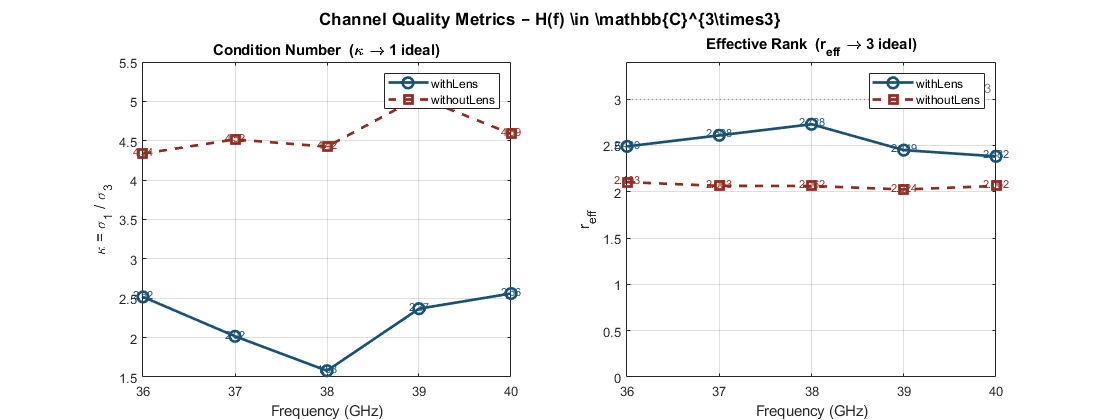
\includegraphics[width=0.85\textwidth]{image/evaluation_result_channelQualityMetrics.png}
    \caption{Evaluation result of the communication metrics based on the SVD-derived channel quality metrics.}
    \label{fig:evaluation_communication_metrics}
\end{figure}

Therefore, the with-lens case shows better angular separability, with the best result observed at
38 GHz \((\kappa=1.579,\ r_{\mathrm{eff}}=2.7279)\).

\subsubsection{CSI-Based Communication Metrics}

The communication metrics are evaluated from the same angular-domain CSI matrix
\(\mathbf{H}_{\theta}(f)\). The indices are kept consistent with the channel formulation: \(i\)
denotes the RX port, \(j\) denotes the incident-angle state, and
\(\theta_j\in\{0^\circ,+45^\circ,-45^\circ\}\). The CSI coefficient is

\begin{equation}
h_{i,j}(f)
=
S_{\mathrm{rx}i,\mathrm{tx2}}^{\theta_j}(f).
\label{eq:csi_coefficient_capacity}
\end{equation}

\paragraph{A. Single RX-Angle Link Metric}

For one RX port and one incident-angle state, the link metric is written as

\begin{equation}
C_{i,j}(f)
=
\log_2
\left(
1+\rho\left|h_{i,j}(f)\right|^2
\right),
\label{eq:single_angle_capacity}
\end{equation}

where \(\rho\) is the linear SNR. This metric compares the received channel quality for each
individual pair \((\mathrm{rx}i,\theta_j)\).

\begin{figure}[H]
    \centering
    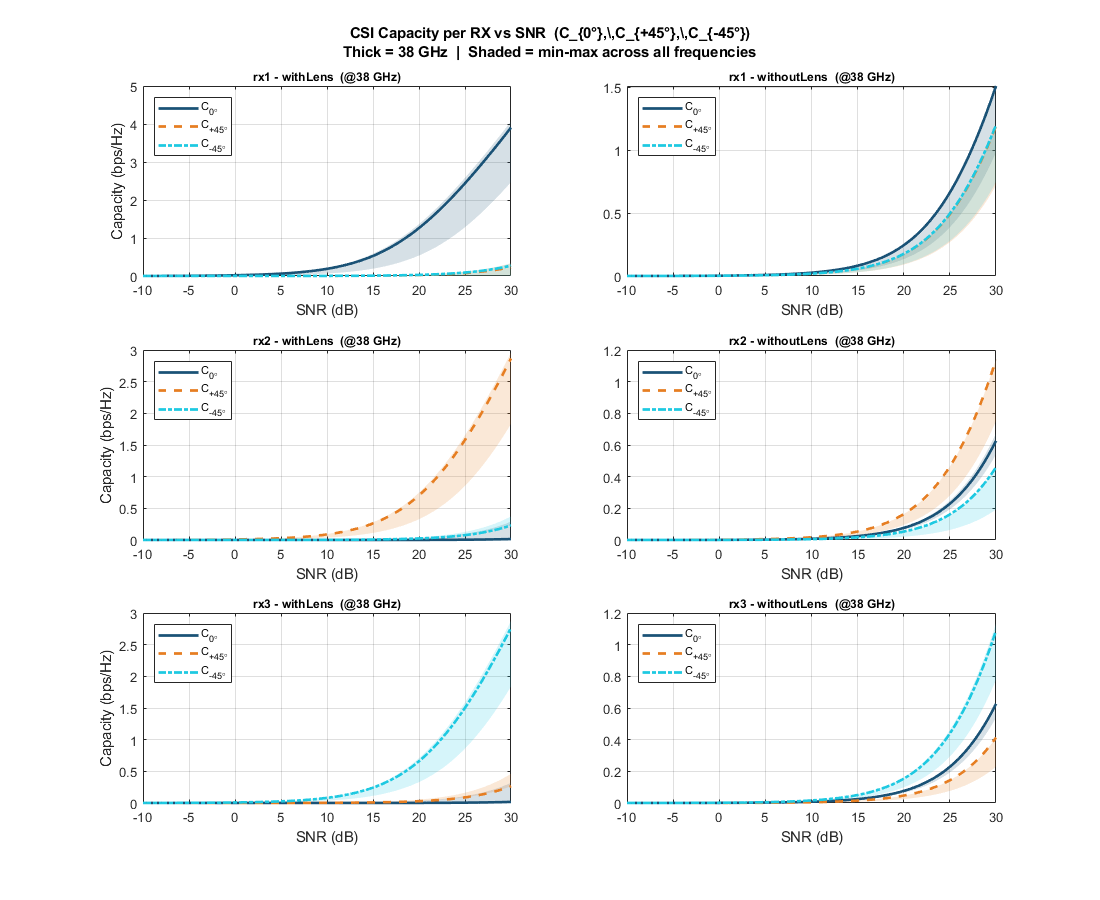
\includegraphics[width=0.95\textwidth]{image/evaluation_result_CSICap_perRXvsSNR.png}
    \caption{Per-RX CSI capacity metric versus SNR for each incident-angle state at 38 GHz.}
    \label{fig:csi_capacity_per_rx_snr}
\end{figure}

Figure~\ref{fig:csi_capacity_per_rx_snr} shows the CSI capacity metric for each RX port under the
three incident-angle states. In the with-lens case, the dominant response follows the intended
angular mapping: RX1 is strongest for \(0^\circ\), RX2 is strongest for \(+45^\circ\), and RX3 is
strongest for \(-45^\circ\). This confirms that the lens response is angle selective and that the
constructed CSI matrix preserves the relationship between incident direction and RX observation
point. The without-lens case shows lower capacity values and weaker angular separation.

\paragraph{B. Per-RX Angular Combining Metric}

For each RX port, the response across the three measured incident-angle states is summarized as

\begin{equation}
C_i^{\mathrm{comb}}(f)
=
\log_2
\left(
1+
\rho
\sum_{j=1}^{N_{\theta}}
\left|h_{i,j}(f)\right|^2
\right),
\label{eq:angular_combining_capacity}
\end{equation}

with \(N_{\theta}=3\). In the current setup,

\begin{equation}
C_i^{\mathrm{comb}}(f)
=
\log_2
\left(
1+
\rho
\left(
\left|S_{\mathrm{rx}i,\mathrm{tx2}}^{0^\circ}(f)\right|^2+
\left|S_{\mathrm{rx}i,\mathrm{tx2}}^{+45^\circ}(f)\right|^2+
\left|S_{\mathrm{rx}i,\mathrm{tx2}}^{-45^\circ}(f)\right|^2
\right)
\right).
\label{eq:angular_combining_capacity_three}
\end{equation}

This metric is used as a per-RX angular response indicator, because the three incident-angle states
are measured sequentially.

\begin{figure}[H]
    \centering
    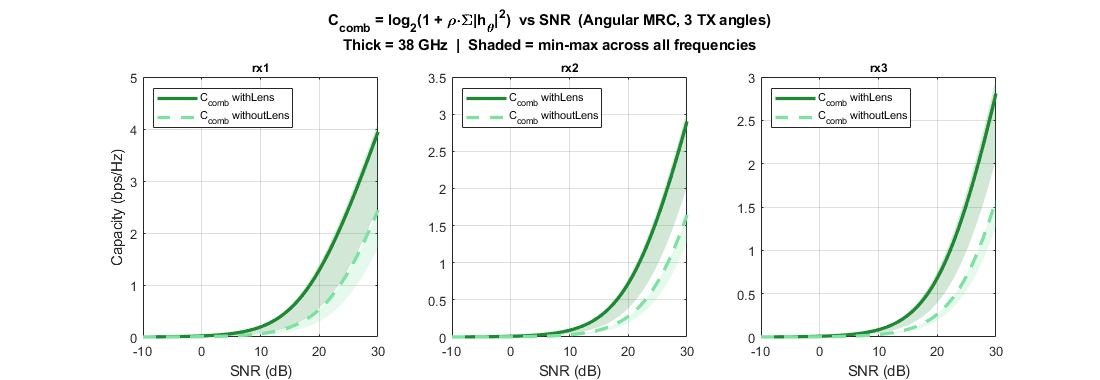
\includegraphics[width=0.95\textwidth]{image/evaluation_result_CSICap_Combine.png}
    \caption{Per-RX angular combining capacity metric for the with-lens and without-lens cases.}
    \label{fig:csi_capacity_combined}
\end{figure}

Figure~\ref{fig:csi_capacity_combined} summarizes the combined angular response for each RX port.
Across all RX positions, the with-lens case provides a higher combining metric than the without-lens
case, especially at higher SNR. This indicates that the antenna lens increases the usable
angular-domain response collected by each RX port. Since the incident angles are measured
sequentially, this result is interpreted as an angular-domain CSI comparison rather than a
simultaneous multi-transmitter capacity result.

\subsubsection{Implementation of Correlation and Decorrelation Metrics}

To quantify the similarity between the measured incident-angle responses, the correlation metric is
computed using the same CSI coefficient notation defined earlier,
\(h_{i,j}(f)=S_{\mathrm{rx}i,\mathrm{tx2}}^{\theta_j}(f)\). For a fixed RX port \(i\), the
frequency responses from all incident-angle states are arranged as

\begin{equation}
\mathbf{A}_{i}
=
\begin{bmatrix}
h_{i,1}(f_1) & h_{i,2}(f_1) & h_{i,3}(f_1)\\
h_{i,1}(f_2) & h_{i,2}(f_2) & h_{i,3}(f_2)\\
\vdots & \vdots & \vdots\\
h_{i,1}(f_{N_f}) & h_{i,2}(f_{N_f}) & h_{i,3}(f_{N_f})
\end{bmatrix},
\label{eq:Hang_corr}
\end{equation}

where \(\mathbf{A}_{i}\in\mathbb{C}^{N_f\times N_{\theta}}\), \(N_f\) is the number of frequency
points, and \(N_{\theta}=3\). Each column of \(\mathbf{A}_i\) is the frequency response vector for
one incident-angle state at RX \(i\). The column vector for the \(j\)-th incident angle is denoted as

\begin{equation}
\mathbf{a}_{i,j}
=
\begin{bmatrix}
h_{i,j}(f_1) &
h_{i,j}(f_2) &
\cdots &
h_{i,j}(f_{N_f})
\end{bmatrix}^{T}.
\label{eq:angular_response_vector_corr}
\end{equation}

The Gram matrix for RX \(i\) is then computed as

\begin{equation}
\mathbf{G}_{i}
=
\mathbf{A}_{i}^{H}
\mathbf{A}_{i},
\label{eq:gram_corr}
\end{equation}

where \((\cdot)^H\) denotes the Hermitian transpose.

The diagonal elements of \(\mathbf{G}_{i}\) are used to obtain the norm of each angular response
vector:

\begin{equation}
d_{i,j}
=
\sqrt{\left[\mathbf{G}_{i}\right]_{j,j}}
=
\left\|\mathbf{a}_{i,j}\right\|_2.
\label{eq:d_corr}
\end{equation}

The normalized correlation between the \(j\)-th and \(m\)-th incident-angle responses at RX \(i\) is

\begin{equation}
\Phi_{i,jm}
=
\frac{\left|\left[\mathbf{G}_{i}\right]_{j,m}\right|}
{d_{i,j}d_{i,m}}
=
\frac{\left|\mathbf{a}_{i,j}^{H}\mathbf{a}_{i,m}\right|}
{\left\|\mathbf{a}_{i,j}\right\|_2\left\|\mathbf{a}_{i,m}\right\|_2},
\label{eq:normalized_complex_corr}
\end{equation}

where \(j\neq m\) and \(j,m\in\{1,2,3\}\). The coefficient \(\Phi_{i,jm}\) satisfies

\begin{equation}
0 \leq \Phi_{i,jm} \leq 1.
\end{equation}

A value close to unity indicates that two angular responses are highly similar, whereas a value close to zero indicates that the two responses are nearly orthogonal and therefore more easily distinguishable.

It should be noted that the magnitude operator in \eqref{eq:normalized_complex_corr} removes the
effect of global phase rotation. Therefore, the metric evaluates the similarity of the angular
response pattern across frequency, not only the absolute phase offset between two incident-angle
states.

To summarize the correlation level for RX \(i\), the average off-diagonal angular correlation is

\begin{equation}
\overline{\Phi}_{i}
=
\frac{1}{N_{\theta}(N_{\theta}-1)}
\sum_{j=1}^{N_{\theta}}
\sum_{\substack{m=1\\m\neq j}}^{N_{\theta}}
\Phi_{i,jm},
\label{eq:avg_corr}
\end{equation}

and the corresponding decorrelation score is defined as

\begin{equation}
D_i
=
1-\overline{\Phi}_{i}.
\label{eq:decorrelation_metric}
\end{equation}

The decorrelation score satisfies

\begin{equation}
0 \leq D_i \leq 1.
\end{equation}

When all angular responses are highly correlated,

\begin{equation}
\Phi_{i,jm}\approx 1,
\end{equation}

the decorrelation score approaches

\begin{equation}
D_i \approx 0.
\end{equation}

Conversely, when the angular responses are nearly orthogonal,

\begin{equation}
\Phi_{i,jm}\approx 0,
\end{equation}

the decorrelation score approaches

\begin{equation}
D_i \approx 1.
\end{equation}

Therefore, larger values of \(D_i\) indicate stronger angular decorrelation and improved angular
separability at RX \(i\).

The normalized correlation coefficient in \eqref{eq:normalized_complex_corr} is consistent with the
normalized inner-product formulation commonly used in channel analysis and antenna diversity
evaluation. The decorrelation score in \eqref{eq:decorrelation_metric} is used as a compact scalar
indicator for comparing the with-lens and without-lens angular-domain CSI responses.

The same normalized inner-product formulation is also used to evaluate cross-RX correlation for a
fixed incident-angle state. For incident angle \(\theta_j\), the frequency response vector observed at
RX \(i\) is defined as

\begin{equation}
\mathbf{b}_{i,j}
=
\begin{bmatrix}
h_{i,j}(f_1) &
h_{i,j}(f_2) &
\cdots &
h_{i,j}(f_{N_f})
\end{bmatrix}^{T}.
\label{eq:cross_rx_response_vector}
\end{equation}

The normalized cross-RX correlation between RX \(i\) and RX \(m\) for the same incident-angle state
\(\theta_j\) is then written as

\begin{equation}
\Psi_{j,im}
=
\frac{\left|\mathbf{b}_{i,j}^{H}\mathbf{b}_{m,j}\right|}
{\left\|\mathbf{b}_{i,j}\right\|_2\left\|\mathbf{b}_{m,j}\right\|_2},
\qquad i\neq m.
\label{eq:cross_rx_correlation}
\end{equation}

\begin{figure}[H]
    \centering
    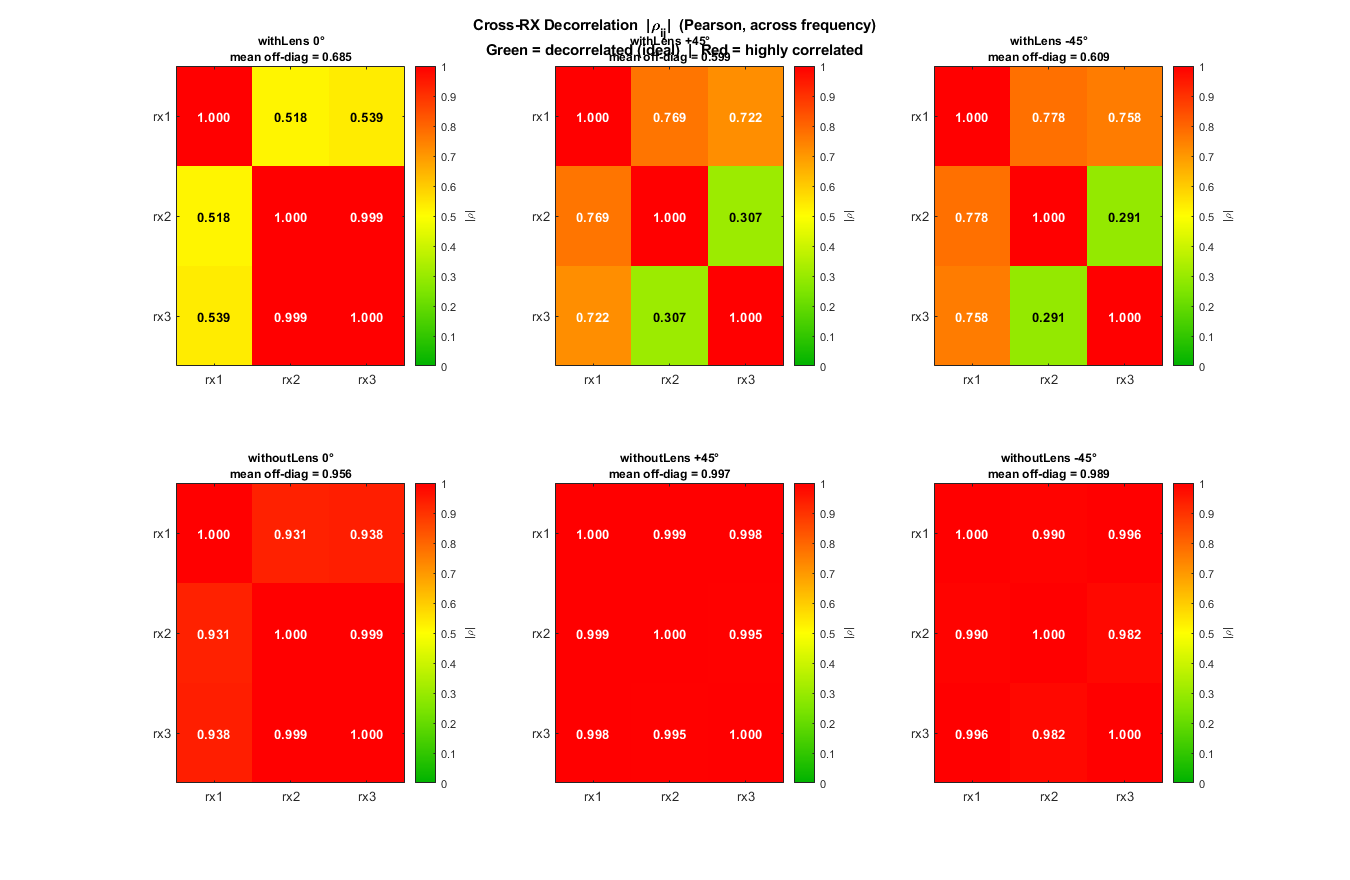
\includegraphics[width=0.95\textwidth]{image/evaluation_result_corelation.png}
    \caption{Cross-RX correlation and decorrelation result for the with-lens and without-lens cases.}
    \label{fig:correlation_decorrelation_result}
\end{figure}

Figure~\ref{fig:correlation_decorrelation_result} shows that the without-lens case produces highly
correlated RX responses, with most off-diagonal correlation values close to unity. This means that
the RX ports observe very similar frequency response patterns without the antenna lens. In contrast,
the with-lens case reduces the off-diagonal correlation for several incident-angle conditions,
especially between RX2 and RX3 at \(+45^\circ\) and \(-45^\circ\). This indicates stronger cross-RX
decorrelation and better spatial-angular separation when the antenna lens is included.

\section{Simulation Antenna Lens 3TX to 3RX with Ray-Trace Method on HFSS SBR+}

\subsection{Experimental Setup}

\begin{figure}[H]
    \centering
    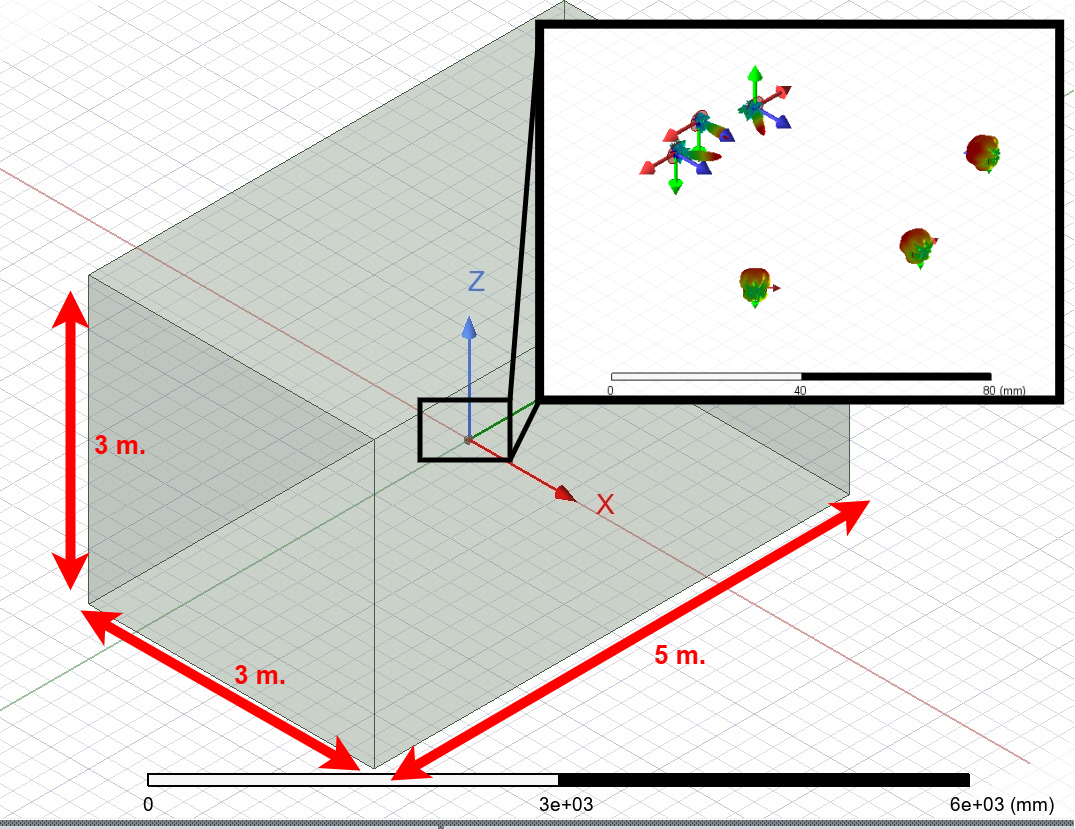
\includegraphics[width=0.85\textwidth]{image/Room_SBR_withCloseup.png}
    \caption{SBR+ simulation room and close-up view of the 3TX-to-3RX antenna lens setup.}
    \label{fig:sbr_room_closeup}
\end{figure}

The SBR+ simulation was prepared as a propagation-level study for a physical 3TX-to-3RX antenna lens
configuration, as shown in Fig.~\ref{fig:sbr_room_closeup}. In this setup, the three TX sources
represent different physical illumination
directions, while RX1, RX2, and RX3 are used as observation points behind the lens. The purpose of
this simulation is to observe the dominant propagation paths, focusing direction, and received
channel behavior produced by the antenna lens under multiple TX/RX combinations.
The simulation was performed from 37 GHz to 39 GHz with a 1 GHz frequency step, resulting in three
evaluated frequency points: 37 GHz, 38 GHz, and 39 GHz.

\begin{table}[H]
    \centering
    \caption{SBR+ simulation configuration for the physical 3TX-to-3RX setup.}
    \label{tab:sbr_simulation_setup}
    \begin{tabular}{lll}
        \hline
        \textbf{Element} & \textbf{Role} & \textbf{Evaluation Purpose} \\
        \hline
        TX1--TX3 & Physical source positions & Illuminate the lens from multiple TX locations \\
        RX1--RX3 & Receiver observation points & Observe the received response behind the lens \\
        Antenna lens & Focusing structure & Redirect and focus the incident propagation paths \\
        Frequency sweep & 37--39 GHz, 1 GHz step & Evaluate the channel response across the target band \\
        HFSS SBR+ & Ray-trace solver & Evaluate dominant paths and high-frequency propagation \\
        \hline
    \end{tabular}
\end{table}

The detailed SBR+ setup, including the TX distance, antenna lens position, focal radius, and RX
angular placement, is shown in Fig.~\ref{fig:sbr_detailed_setup}. This view is used as the reference
geometry for the 3TX-to-3RX evaluation.

\begin{figure}[H]
    \centering
    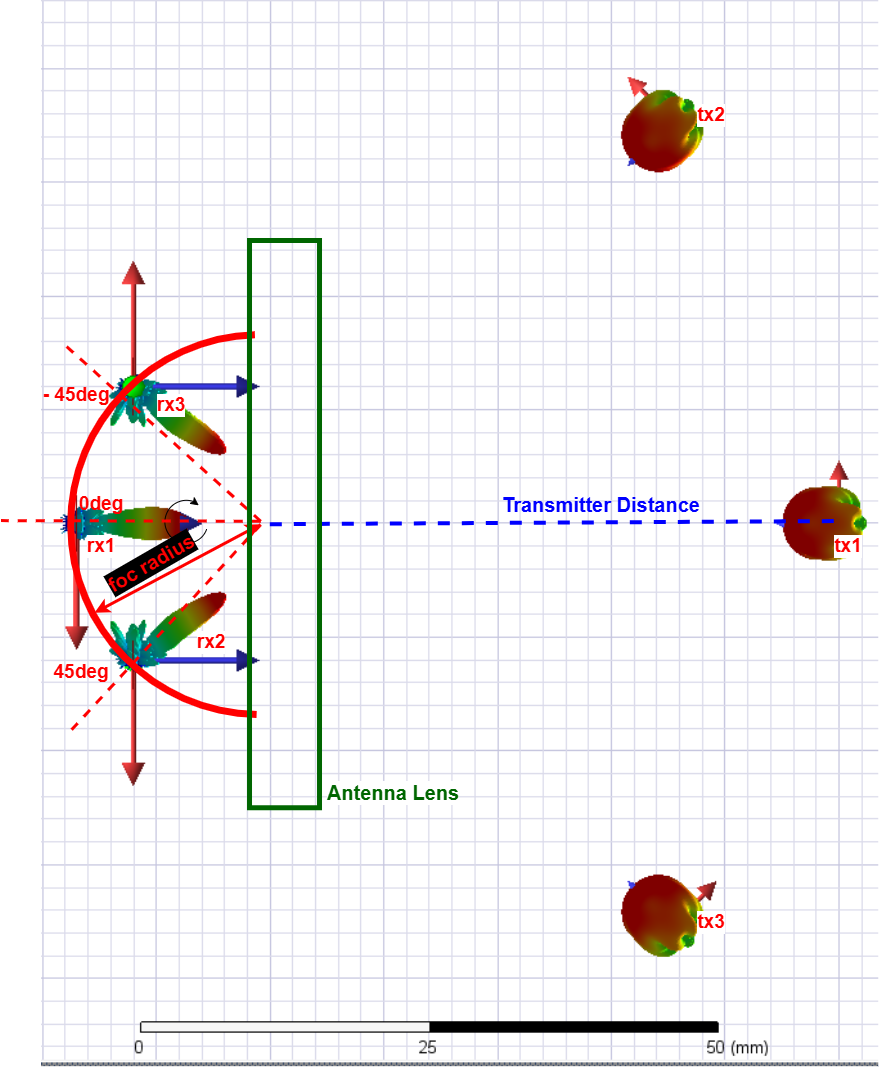
\includegraphics[width=0.85\textwidth]{image/SetupEnvirontment_SBR_WithLens_up_edited.PNG}
    \caption{Detailed SBR+ setup showing TX placement, antenna lens position, focal radius, and RX observation angles.}
    \label{fig:sbr_detailed_setup}
\end{figure}

The radiation pattern representation used in the SBR+ setup was evaluated for two configurations:
with the antenna lens and without the antenna lens. These two cases are shown in
Fig.~\ref{fig:sbr_radiation_pattern_setup}.

\begin{figure}[H]
    \centering
    \begin{minipage}{0.48\textwidth}
        \centering
        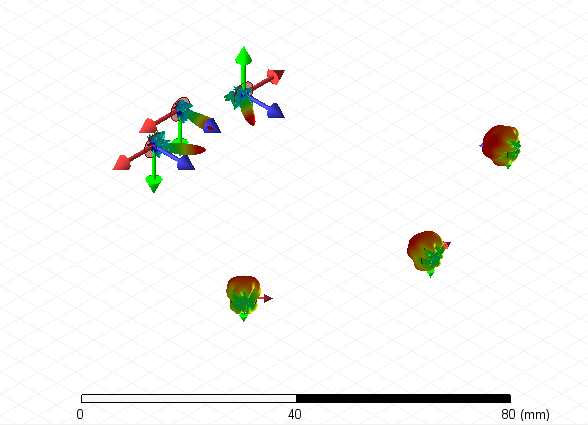
\includegraphics[width=\textwidth]{image/SetupEnvirontment_SBR_WithLens.PNG}
        \caption*{(a) Radiation pattern with antenna lens}
    \end{minipage}
    \hfill
    \begin{minipage}{0.48\textwidth}
        \centering
        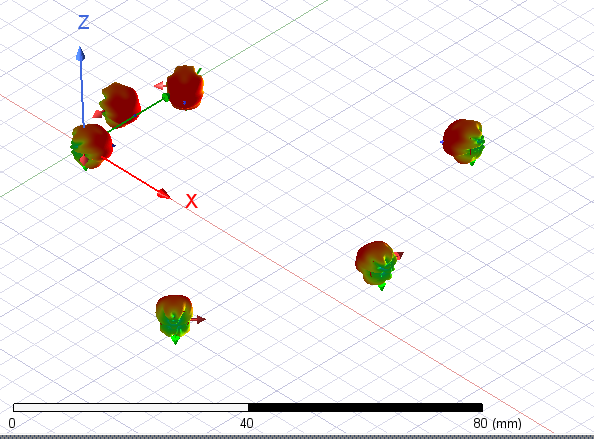
\includegraphics[width=\textwidth]{image/SetupEnvirontment_SBR_WithoutLens.PNG}
        \caption*{(b) Radiation pattern without antenna lens}
    \end{minipage}
    \caption{Radiation pattern representation in the SBR+ experimental setup with and without the antenna lens.}
    \label{fig:sbr_radiation_pattern_setup}
\end{figure}

\subsection{Result}

The main result of the SBR+ simulation is the TX-to-RX S-parameter magnitude response, as shown in
Fig.~\ref{fig:sbr_sparam_result}. This result compares the transmission coefficient from each TX
source to RX1, RX2, and RX3 for both the with-lens and without-lens cases. Therefore, the graph is
used as the primary reference to evaluate how the antenna lens changes the received channel response
across the 3TX-to-3RX configuration.

\begin{figure}[H]
    \centering
    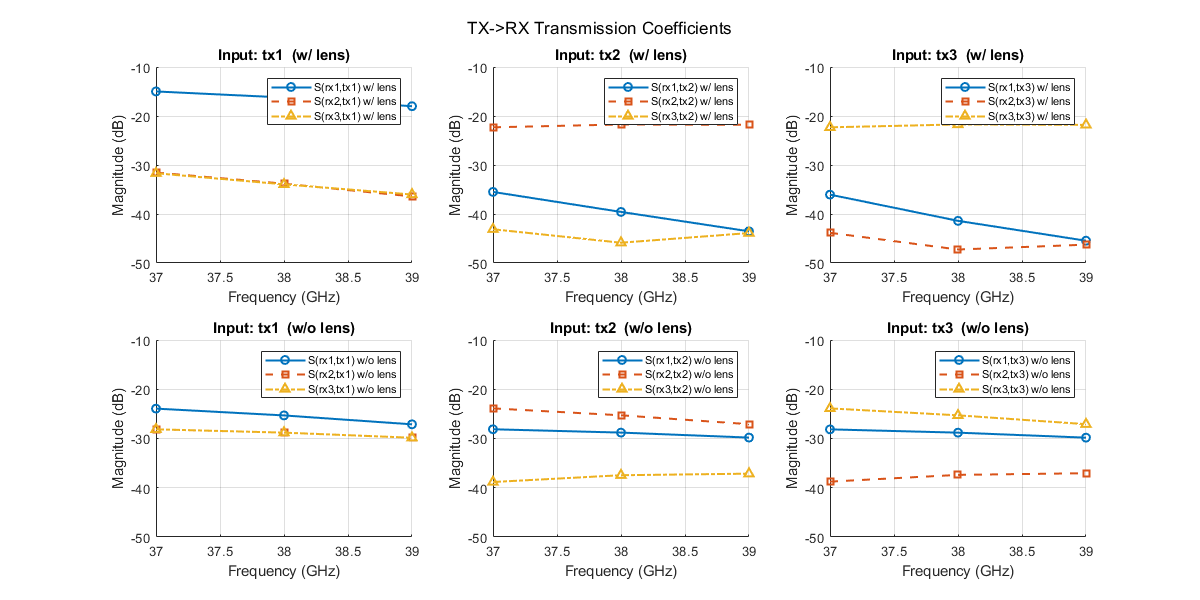
\includegraphics[width=0.95\textwidth]{image/Result_SBR_SParam_db.png}
    \caption{SBR+ TX-to-RX S-parameter magnitude response for the with-lens and without-lens cases.}
    \label{fig:sbr_sparam_result}
\end{figure}

Figure~\ref{fig:sbr_sparam_result} shows that the antenna lens changes the dominant TX-to-RX
coupling pattern. In the with-lens case, several TX/RX pairs show higher received magnitude than the
corresponding without-lens case, indicating that the lens increases the coupling for specific
TX-to-RX directions. In contrast, the without-lens case shows a weaker separation between several
channel responses. This confirms that the S-parameter graph can be used as direct evidence of the
lens-induced channel change before the response is quantified further in the evaluation section.

\subsection{Evaluation}

The SBR+ evaluation compares the radiation-pattern configurations shown in
Fig.~\ref{fig:sbr_radiation_pattern_setup}. The with-lens and without-lens configurations use the
same TX and RX positions. Therefore, the
differences observed in the following metrics are interpreted as the lens-induced change in the
measured S-parameter-based channel response.

\subsubsection{S-Parameter-Based Communication Channel Evaluation}

In this work, the measured S-parameters are used to construct an empirical frequency-domain communication channel. 
For each frequency point, the MIMO channel matrix is defined as
\begin{equation}
    \mathbf{H}(f) \in \mathbb{C}^{N_R \times N_T},
\end{equation}
where \(N_R\) is the number of receive ports and \(N_T\) is the number of transmit ports. 
Each element of the channel matrix is obtained from the measured transmission coefficient between the corresponding transmit and receive ports:
\begin{equation}
    H_{ij}(f) = S(\mathrm{rx}_i,\mathrm{tx}_j;f),
\end{equation}
where \(S(\mathrm{rx}_i,\mathrm{tx}_j;f)\) denotes the complex S-parameter from the \(j\)-th transmit port to the \(i\)-th receive port at frequency \(f\).

For the \(3 \times 3\) measurement configuration used in this work, the channel matrix is written as
\begin{equation}
\mathbf{H}(f)
=
\begin{bmatrix}
S(\mathrm{rx1},\mathrm{tx1}) & S(\mathrm{rx1},\mathrm{tx2}) & S(\mathrm{rx1},\mathrm{tx3}) \\
S(\mathrm{rx2},\mathrm{tx1}) & S(\mathrm{rx2},\mathrm{tx2}) & S(\mathrm{rx2},\mathrm{tx3}) \\
S(\mathrm{rx3},\mathrm{tx1}) & S(\mathrm{rx3},\mathrm{tx2}) & S(\mathrm{rx3},\mathrm{tx3})
\end{bmatrix}.
\end{equation}

The corresponding frequency-domain input-output relation can be expressed as
\begin{equation}
    \mathbf{y}(f) = \mathbf{H}(f)\mathbf{x}(f) + \mathbf{n}(f),
\end{equation}
where
\begin{equation}
    \mathbf{x}(f) \in \mathbb{C}^{N_T \times 1}
\end{equation}
is the transmitted signal vector or incident-mode excitation vector,
\begin{equation}
    \mathbf{y}(f) \in \mathbb{C}^{N_R \times 1}
\end{equation}
is the received signal vector, and \(\mathbf{n}(f)\) denotes the additive noise vector.

It should be noted that \(\mathbf{H}(f)\) in this formulation represents a measured end-to-end RF channel response. 
Therefore, it does not only describe the pure free-space propagation channel, but also includes the effects of the transmit antenna, receive antenna, lens response, propagation path, mutual coupling, impedance mismatch, and measurement reference plane. 
Thus, the proposed formulation is more accurately described as an S-parameter-based empirical communication channel evaluation.

\subsubsection{Singular Value Decomposition of the Channel Matrix}

After constructing the channel matrix, singular value decomposition is applied to \(\mathbf{H}(f)\) at each frequency point:
\begin{equation}
    \mathbf{H}(f)
    =
    \mathbf{U}(f)
    \boldsymbol{\Sigma}(f)
    \mathbf{V}^{H}(f),
\end{equation}
where \(\mathbf{U}(f)\) and \(\mathbf{V}(f)\) are unitary matrices, and \(\boldsymbol{\Sigma}(f)\) contains the singular values of the channel matrix.

For a \(3 \times 3\) channel, the singular-value matrix can be written as
\begin{equation}
    \boldsymbol{\Sigma}(f)
    =
    \mathrm{diag}
    \left(
    \sigma_1(f),
    \sigma_2(f),
    \sigma_3(f)
    \right),
\end{equation}
with
\begin{equation}
    \sigma_1(f) \geq \sigma_2(f) \geq \sigma_3(f) \geq 0.
\end{equation}

The singular value \(\sigma_i(f)\) represents the amplitude gain of the \(i\)-th equivalent parallel MIMO eigenchannel, while \(\sigma_i^2(f)\) represents the corresponding power gain. 
If only \(\sigma_1(f)\) is dominant, the channel is mainly supported by one spatial mode. 
In contrast, if \(\sigma_1(f)\), \(\sigma_2(f)\), and \(\sigma_3(f)\) have comparable values, the channel provides better spatial multiplexing capability.

Two additional indicators are extracted from the same singular values. The condition number is used
to measure the balance of the MIMO eigenmodes:
\begin{equation}
    \kappa(f)
    =
    \frac{\sigma_1(f)}
    {\sigma_3(f)}.
\end{equation}
A lower \(\kappa(f)\) indicates that the channel modes are more balanced. The effective rank is used
to estimate the effective number of active spatial modes:
\begin{equation}
    p_i(f)
    =
    \frac{\sigma_i^2(f)}
    {\sum_{k=1}^{3}\sigma_k^2(f)},
    \qquad
    r_{\mathrm{eff}}(f)
    =
    \exp
    \left(
    -\sum_{i=1}^{3}p_i(f)\ln p_i(f)
    \right).
\end{equation}
For a \(3\times3\) channel, \(r_{\mathrm{eff}}(f)\) ranges from 1 to 3. A value closer to 3 indicates
that more spatial modes contribute to the channel response.

The extracted SVD results from the SBR+ channel matrices are summarized in
Table~\ref{tab:sbr_svd_summary}. The table compares the with-lens and without-lens datasets at
37--39 GHz using the three singular values, condition number, effective rank, and the equal-power
capacity indicator at 20 dB.

\begin{table}[H]
    \centering
    \caption{Extracted SVD summary of the SBR+ \(3\times3\) channel matrix.}
    \label{tab:sbr_svd_summary}
    \footnotesize
    \setlength{\tabcolsep}{4pt}
    \resizebox{\textwidth}{!}{%
    \begin{tabular}{lrrrrrrr}
        \hline
        \textbf{Dataset} & \textbf{Freq. (GHz)} & \(\boldsymbol{\sigma_1}\) & \(\boldsymbol{\sigma_2}\) & \(\boldsymbol{\sigma_3}\) & \(\boldsymbol{\kappa}\) & \(\boldsymbol{r_{\mathrm{eff}}}\) & \(\boldsymbol{C_{20\mathrm{dB}}}\) \\
        \hline
        With Lens    & 37 & 0.186 & 0.082 & 0.064 & 2.89 & 2.030 & 1.584 \\
        Without Lens & 37 & 0.124 & 0.055 & 0.016 & 7.61 & 1.680 & 0.747 \\
        \hline
        With Lens    & 38 & 0.160 & 0.087 & 0.072 & 2.22 & 2.363 & 1.443 \\
        Without Lens & 38 & 0.111 & 0.042 & 0.018 & 6.25 & 1.608 & 0.597 \\
        \hline
        With Lens    & 39 & 0.130 & 0.087 & 0.072 & 1.81 & 2.646 & 1.199 \\
        Without Lens & 39 & 0.096 & 0.031 & 0.017 & 5.58 & 1.534 & 0.443 \\
        \hline
    \end{tabular}%
    }
\end{table}

Table~\ref{tab:sbr_svd_summary} shows that the with-lens case consistently produces stronger and
more balanced singular values than the without-lens case. The condition number decreases from
7.61 to 2.89 at 37 GHz, from 6.25 to 2.22 at 38 GHz, and from 5.58 to 1.81 at 39 GHz. This indicates
that the antenna lens does not only increase the dominant channel response, but also improves the
balance among the available spatial modes. The effective rank and \(C_{20\mathrm{dB}}\) are also
higher in the with-lens case at all evaluated frequencies, confirming that the lens-assisted channel
provides better modal diversity and a stronger communication-channel indicator.

\begin{figure}[H]
    \centering
    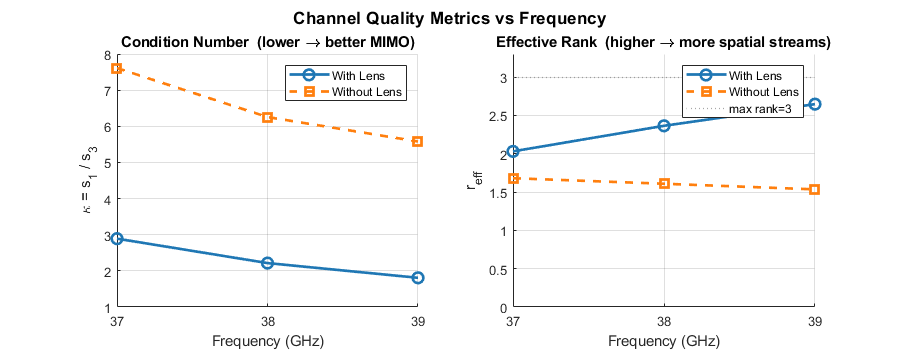
\includegraphics[width=0.9\textwidth]{image/evaluation_SBR_result_channelQualityMetrics.png}
    \caption{SBR+ channel quality metrics based on condition number and effective rank.}
    \label{fig:sbr_channel_quality_metrics}
\end{figure}

Figure~\ref{fig:sbr_channel_quality_metrics} visualizes the same SVD-derived channel-quality trend.
The with-lens case consistently has a lower condition number than the without-lens case, meaning the
three singular modes are less dominated by a single path. At the same time, the effective rank is
higher with the lens and increases from 37 GHz to 39 GHz, showing that the lens-assisted channel uses
more independent spatial modes. This result supports the SVD table: the antenna lens improves both
the modal balance and the spatial diversity of the SBR+ \(3\times3\) channel matrix.

\subsubsection{Equal-Power MIMO Channel Capacity}

The MIMO channel capacity is evaluated assuming equal power allocation across the transmit ports. 
The SNR in decibel scale is first converted into linear scale as
\begin{equation}
    \rho
    =
    10^{\mathrm{SNR}_{\mathrm{dB}}/10}.
\end{equation}

The equal-power MIMO capacity is calculated as
\begin{equation}
    C(f)
    =
    \log_2
    \det
    \left[
    \mathbf{I}_{N_R}
    +
    \frac{\rho}{N_T}
    \mathbf{H}(f)\mathbf{H}^{H}(f)
    \right]
    \quad
    [\mathrm{bps/Hz}].
\end{equation}

Using the singular values of \(\mathbf{H}(f)\), the capacity can be equivalently written as
\begin{equation}
    C(f)
    =
    \sum_{i=1}^{\min(N_R,N_T)}
    \log_2
    \left(
    1+
    \frac{\rho}{N_T}
    \sigma_i^2(f)
    \right)
    \quad
    [\mathrm{bps/Hz}].
\end{equation}

For the \(3 \times 3\) channel used in this work, the expression becomes
\begin{equation}
    C(f)
    =
    \sum_{i=1}^{3}
    \log_2
    \left(
    1+
    \frac{\rho}{3}
    \sigma_i^2(f)
    \right).
\end{equation}

This metric evaluates the achievable spectral efficiency of the measured channel. 
If the lens increases the transmission magnitude, the singular values tend to increase, which can improve the raw channel capacity. 
Furthermore, if the lens improves spatial decorrelation, the weaker singular values \(\sigma_2(f)\) and \(\sigma_3(f)\) may increase relative to \(\sigma_1(f)\), resulting in better MIMO capacity.

\begin{figure}[H]
    \centering
    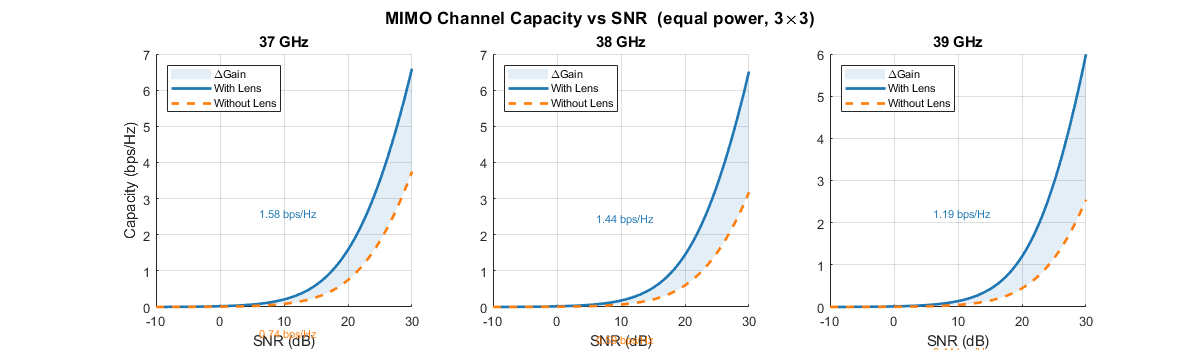
\includegraphics[width=0.95\textwidth]{image/evaluation_result_SBR_CSICHannelCapacity.png}
    \caption{SBR+ MIMO channel capacity versus SNR for the with-lens and without-lens cases.}
    \label{fig:sbr_capacity_vs_snr}
\end{figure}

Figure~\ref{fig:sbr_capacity_vs_snr} shows that the with-lens channel provides higher capacity than
the without-lens channel at 37, 38, and 39 GHz. The capacity gain becomes more visible as SNR
increases, because the stronger singular values and improved modal balance contribute more directly
to the achievable spectral efficiency.

\subsubsection{Receive-Side Spatial Correlation}

The receive-side spatial correlation matrix is calculated as
\begin{equation}
    \mathbf{R}_{\mathrm{rx}}(f)
    =
    \mathbf{H}(f)\mathbf{H}^{H}(f).
\end{equation}

The normalized receive-side spatial correlation coefficient between the \(i\)-th and \(k\)-th receive ports is given by
\begin{equation}
    \rho_{ik}^{\mathrm{rx}}(f)
    =
    \frac{
    R_{\mathrm{rx},ik}(f)
    }
    {
    \sqrt{
    R_{\mathrm{rx},ii}(f)
    R_{\mathrm{rx},kk}(f)
    }
    }.
\end{equation}

The magnitude \(|\rho_{ik}^{\mathrm{rx}}(f)|\) is used to evaluate the correlation level. 
A value close to zero indicates good receive-side decorrelation, while a value close to one indicates that the receive ports observe highly similar channel responses.

\subsubsection{Transmit-Side Spatial Correlation}

The transmit-side spatial correlation matrix is calculated as
\begin{equation}
    \mathbf{R}_{\mathrm{tx}}(f)
    =
    \mathbf{H}^{H}(f)\mathbf{H}(f).
\end{equation}

The normalized transmit-side spatial correlation coefficient between the \(j\)-th and \(l\)-th transmit ports is given by
\begin{equation}
    \rho_{jl}^{\mathrm{tx}}(f)
    =
    \frac{
    R_{\mathrm{tx},jl}(f)
    }
    {
    \sqrt{
    R_{\mathrm{tx},jj}(f)
    R_{\mathrm{tx},ll}(f)
    }
    }.
\end{equation}

A smaller off-diagonal value of \(|\rho_{jl}^{\mathrm{tx}}(f)|\) indicates that the transmit ports generate more distinguishable channel responses. 
This is desirable for MIMO communication because it reduces spatial redundancy between the transmit channels.

\subsubsection{Mean Off-Diagonal Correlation}

To summarize the spatial correlation level using a single scalar metric, the mean off-diagonal correlation is calculated as
\begin{equation}
    \overline{\rho}_{\mathrm{off}}(f)
    =
    \frac{1}{N(N-1)}
    \sum_{i\neq k}
    |\rho_{ik}(f)|.
\end{equation}

Here, \(N\) is the dimension of the correlation matrix. 
For the receive-side correlation matrix, \(N=N_R\), while for the transmit-side correlation matrix, \(N=N_T\). 
A lower value of \(\overline{\rho}_{\mathrm{off}}(f)\) indicates better spatial decorrelation.

\begin{figure}[H]
    \centering
    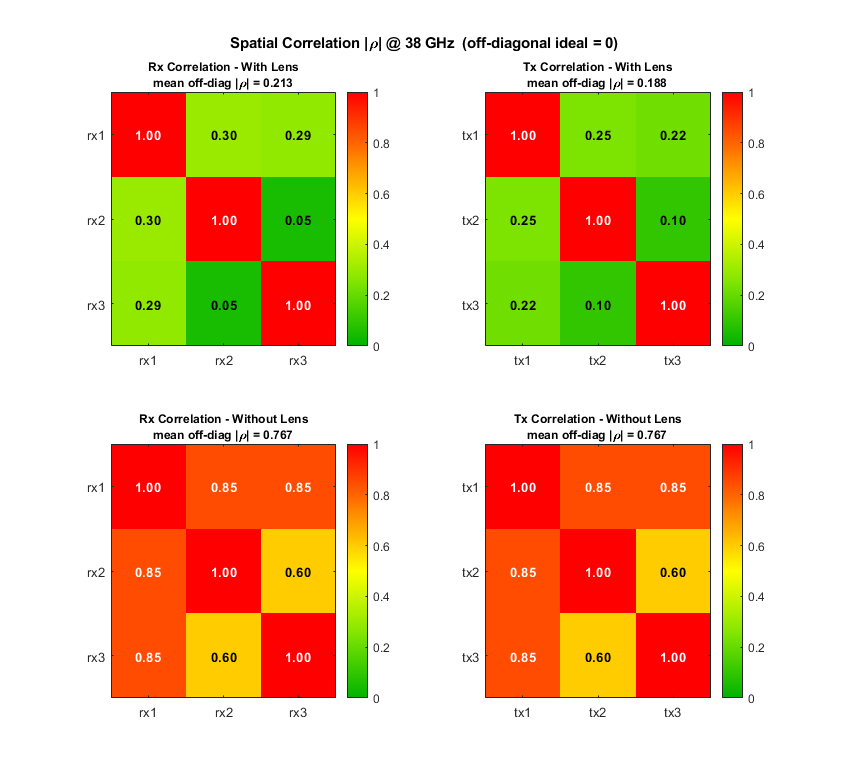
\includegraphics[width=0.9\textwidth]{image/evaluation_SBR_result_corelation.png}
    \caption{SBR+ receive-side and transmit-side spatial correlation comparison at 38 GHz.}
    \label{fig:sbr_spatial_correlation}
\end{figure}

Figure~\ref{fig:sbr_spatial_correlation} shows that the with-lens case reduces the mean
off-diagonal correlation for both the receive-side and transmit-side correlation matrices. At
38 GHz, the mean off-diagonal correlation is approximately 0.213 for the with-lens RX correlation
and 0.188 for the with-lens TX correlation, while the without-lens case is approximately 0.767 for
both sides. This indicates that the antenna lens improves spatial decorrelation and reduces channel
redundancy in the SBR+ 3TX-to-3RX configuration.

\subsubsection{Capacity Evaluation at Fixed SNR}

In addition to evaluating the capacity over a range of SNR values, the program also compares the capacity at fixed SNR points, such as
\begin{equation}
    \mathrm{SNR}=0~\mathrm{dB},\quad
    10~\mathrm{dB},\quad
    20~\mathrm{dB}.
\end{equation}

The corresponding linear SNR values are
\begin{equation}
    0~\mathrm{dB} \rightarrow 1,
    \qquad
    10~\mathrm{dB} \rightarrow 10,
    \qquad
    20~\mathrm{dB} \rightarrow 100.
\end{equation}

At each fixed SNR point, the capacity is calculated as
\begin{equation}
    C(f)
    =
    \sum_i
    \log_2
    \left(
    1+
    \frac{\rho_{\mathrm{lin}}}{N_T}
    \sigma_i^2(f)
    \right).
\end{equation}

This fixed-SNR capacity comparison is used to directly evaluate whether the with-lens configuration provides higher spectral efficiency than the without-lens configuration.

\begin{figure}[H]
    \centering
    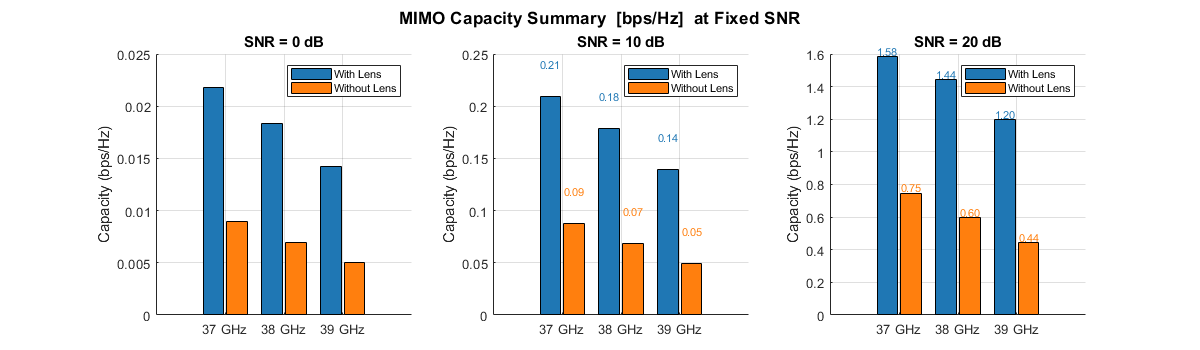
\includegraphics[width=0.95\textwidth]{image/evaluation_result_SBR_MIMOCapacitySummary.png}
    \caption{SBR+ MIMO capacity summary at fixed SNR values for the with-lens and without-lens cases.}
    \label{fig:sbr_capacity_summary}
\end{figure}

Figure~\ref{fig:sbr_capacity_summary} confirms the capacity improvement at fixed SNR points. At
20 dB SNR, the with-lens case reaches approximately 1.58, 1.44, and 1.20 bps/Hz at 37, 38, and
39 GHz, respectively, while the without-lens case remains lower at approximately 0.75, 0.60, and
0.44 bps/Hz. This result is consistent with the lower condition number, higher effective rank, and
lower spatial correlation observed in the with-lens SBR+ channel.

\subsubsection{Summary of the Evaluation Method}

Based on the measured S-parameter data, the program evaluates the communication-channel quality using several MIMO metrics. 
The singular values describe the available spatial eigenmodes, the condition number indicates the balance between those eigenmodes, the effective rank estimates the number of active spatial modes, the spatial correlation matrices quantify the decorrelation level at the transmit and receive sides, and the channel capacity estimates the achievable spectral efficiency.

Therefore, the proposed evaluation is valid as an S-parameter-based empirical communication-channel analysis. 
The resulting channel matrix should be interpreted as a measured end-to-end RF channel response rather than a pure theoretical propagation channel.

% \section*{References}
% \begin{enumerate}[label*=\arabic*.]
%     \item W. Lee et al., “Single-layer phase gradient mmWave metasurface for incident angle independent focusing,” Scientific Reports, 2021. \url{https://www.nature.com/articles/s41598-021-92083-5}
%     \item Prof. Stefano Maci - Metasurface Antenna Design. \url{https://youtu.be/sNEr0r08AvA}
% \end{enumerate}

% \section*{Ethics Declaration}
% I confirm that I have discussed any ethical considerations with my supervision team and, where required, have followed the approval process required by the institution.

%=========================== Appendix ===========================
% \appendix
% \section{Example Floquet Port Simulation Notes}

% \subsection{Example Unit-Cell Setup}
% \begin{table}[H]
%     \centering
%     \caption{Example parameters for a periodic unit-cell simulation.}
%     \begin{tabular}{ll}
%         \hline
%         \textbf{Parameter} & \textbf{Example Value} \\
%         \hline
%         Center frequency & 38 GHz \\
%         Unit-cell period & 3.9 mm \\
%         Substrate thickness & 0.254 mm \\
%         Boundary condition & Master/slave or periodic boundary \\
%         Excitation & Floquet port, normal incidence \\
%         Output target & Transmission phase and magnitude \\
%         \hline
%     \end{tabular}
% \end{table}

% \subsection{Additional Observation Example}
% \begin{itemize}
%     \item The phase response should be checked together with transmission magnitude, because a wide phase range is not useful if the insertion loss is too high.
%     \item The unit-cell boundary must represent an infinite periodic array, not a single isolated radiator.
%     \item A frequency sweep around 35--40 GHz can help identify whether the structure is stable across the target band.
% \end{itemize}

% \subsection{Simulation Checklist Example}
% \begin{enumerate}
%     \item Confirm that the top and bottom Floquet ports are aligned with the propagation direction.
%     \item Verify that the periodic boundaries are assigned to the correct opposite faces.
%     \item Check whether higher-order Floquet modes are propagating or evanescent at the target frequency.
%     \item Export transmission magnitude and phase for comparison between unit-cell variations.
% \end{enumerate}

% \subsection{Reference Notes}
% \begin{enumerate}[label={[\arabic*]}]
%     \item W. Lee et al., ``Single-layer phase gradient mmWave metasurface for incident angle independent focusing,'' \textit{Scientific Reports}, 2021. \url{https://www.nature.com/articles/s41598-021-92083-5}
%     \item Prof. Stefano Maci, ``Metasurface Antenna Design.'' \url{https://youtu.be/sNEr0r08AvA}
%     \item HFSS Floquet port and periodic boundary condition documentation/review notes used for unit-cell simulation setup.
% \end{enumerate}

\section{Comparison of Hybrid, Sionna-RT, and SBR+ Solvers}

\subsection{Comparison Basis and Channel Harmonization}

The three simulation methods are compared using the processed results in
\path{image/channel_comparison_results}. Because the Hybrid model uses
swept incident-angle excitations while Sionna-RT and SBR+ use explicit
transmitter indices, the native antenna names are first mapped to a common
$3\times3$ channel convention. The comparison therefore uses the same
canonical $\mathrm{rx}1$--$\mathrm{rx}3$ and
$\mathrm{tx}1$--$\mathrm{tx}3$ ordering for all solvers. The common anchor
frequencies are 37, 38, and 39~GHz, and both the with-lens and without-lens
conditions are retained.

Two complementary comparisons are required. The raw complex channel matrices
retain absolute path gain and are appropriate for received magnitude and
capacity comparisons. Frobenius-normalized matrices,
\begin{equation}
    \widetilde{\mathbf{H}}
    =\frac{\mathbf{H}}{\lVert\mathbf{H}\rVert_{\mathrm{F}}},
    \label{eq:comparison_frobenius_normalization}
\end{equation}
remove the overall channel-strength difference and are used to compare only
the relative spatial-mode structure. Results from these two normalizations
must not be interpreted interchangeably.

\subsection{Absolute Channel-Magnitude Comparison}

Figures~\ref{fig:comparison_channel_with_magnitude} and
\ref{fig:comparison_channel_without_magnitude} compare the nine canonical
TX--RX coefficients. The figures show that the solvers reproduce the same
broad channel organization, but they do not predict identical absolute
magnitudes. These differences are expected because the methods use different
field formulations, propagation approximations, antenna representations, and
channel-extraction procedures.

\begin{figure}[H]
    \centering
    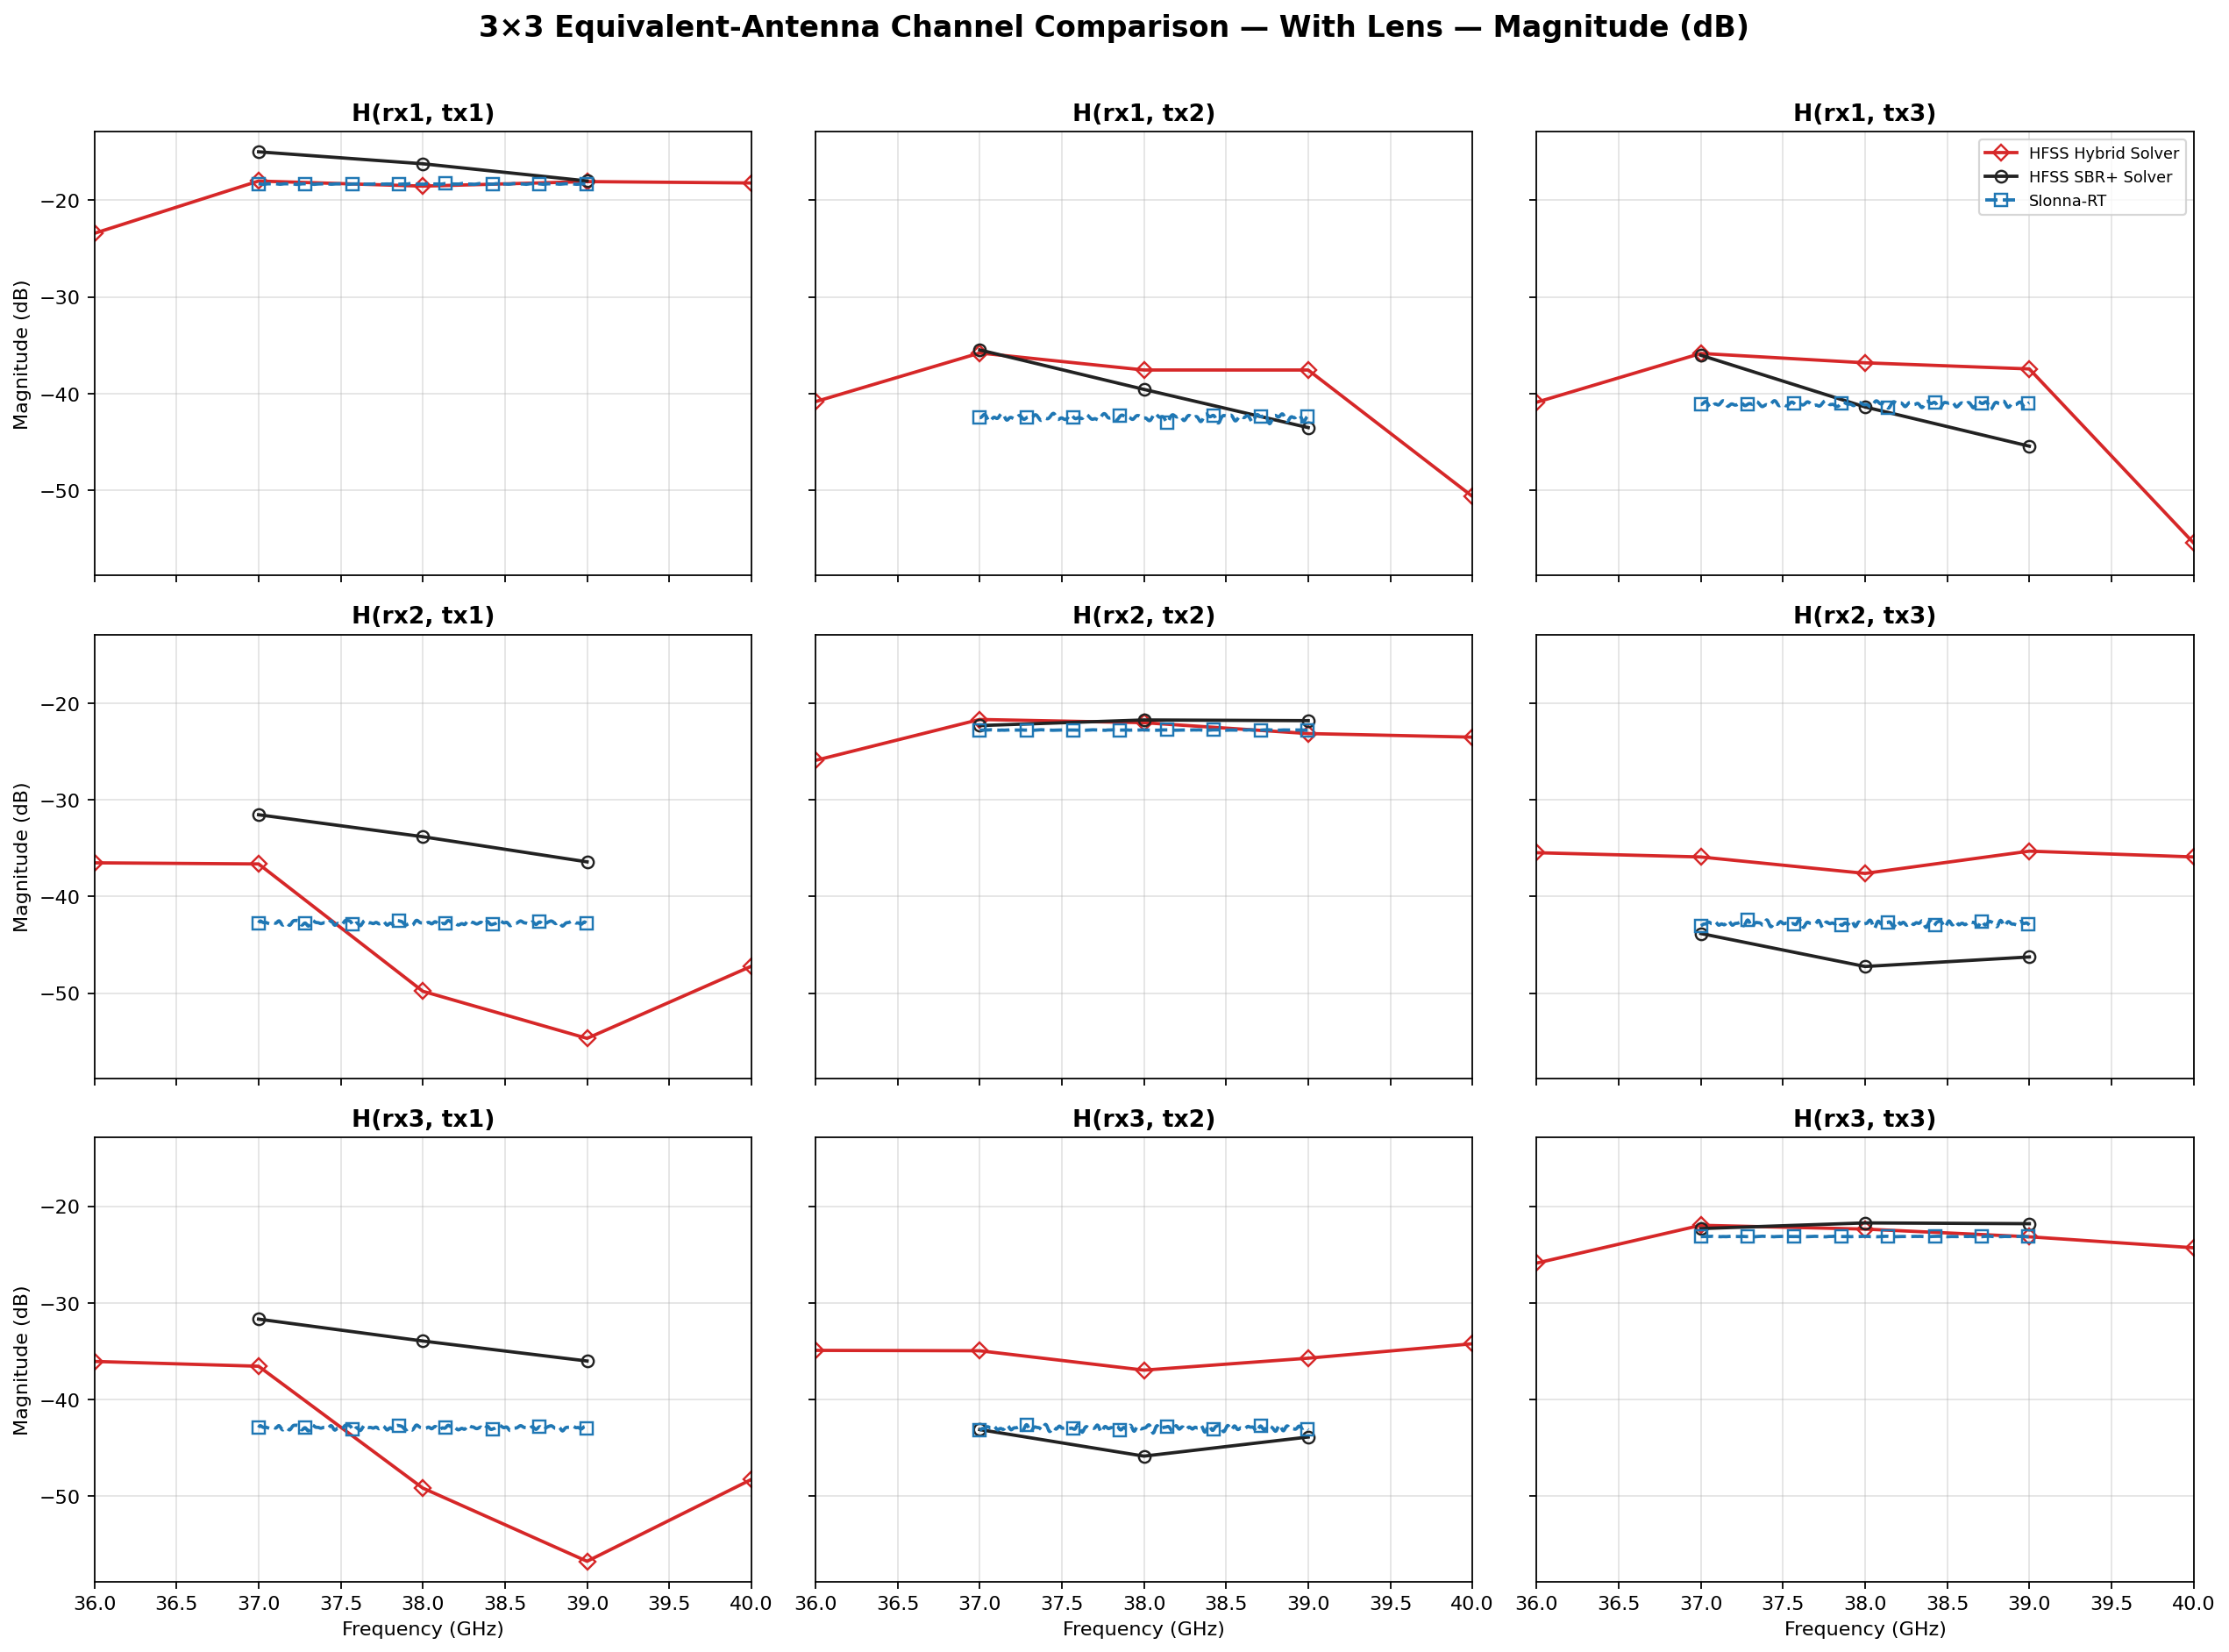
\includegraphics[width=\textwidth]{image/channel_comparison_results/channel_3x3_with_magnitude_db.png}
    \caption{Inter-solver comparison of the $3\times3$ channel magnitudes at
    37, 38, and 39~GHz with the antenna lens.}
    \label{fig:comparison_channel_with_magnitude}
\end{figure}

\begin{figure}[H]
    \centering
    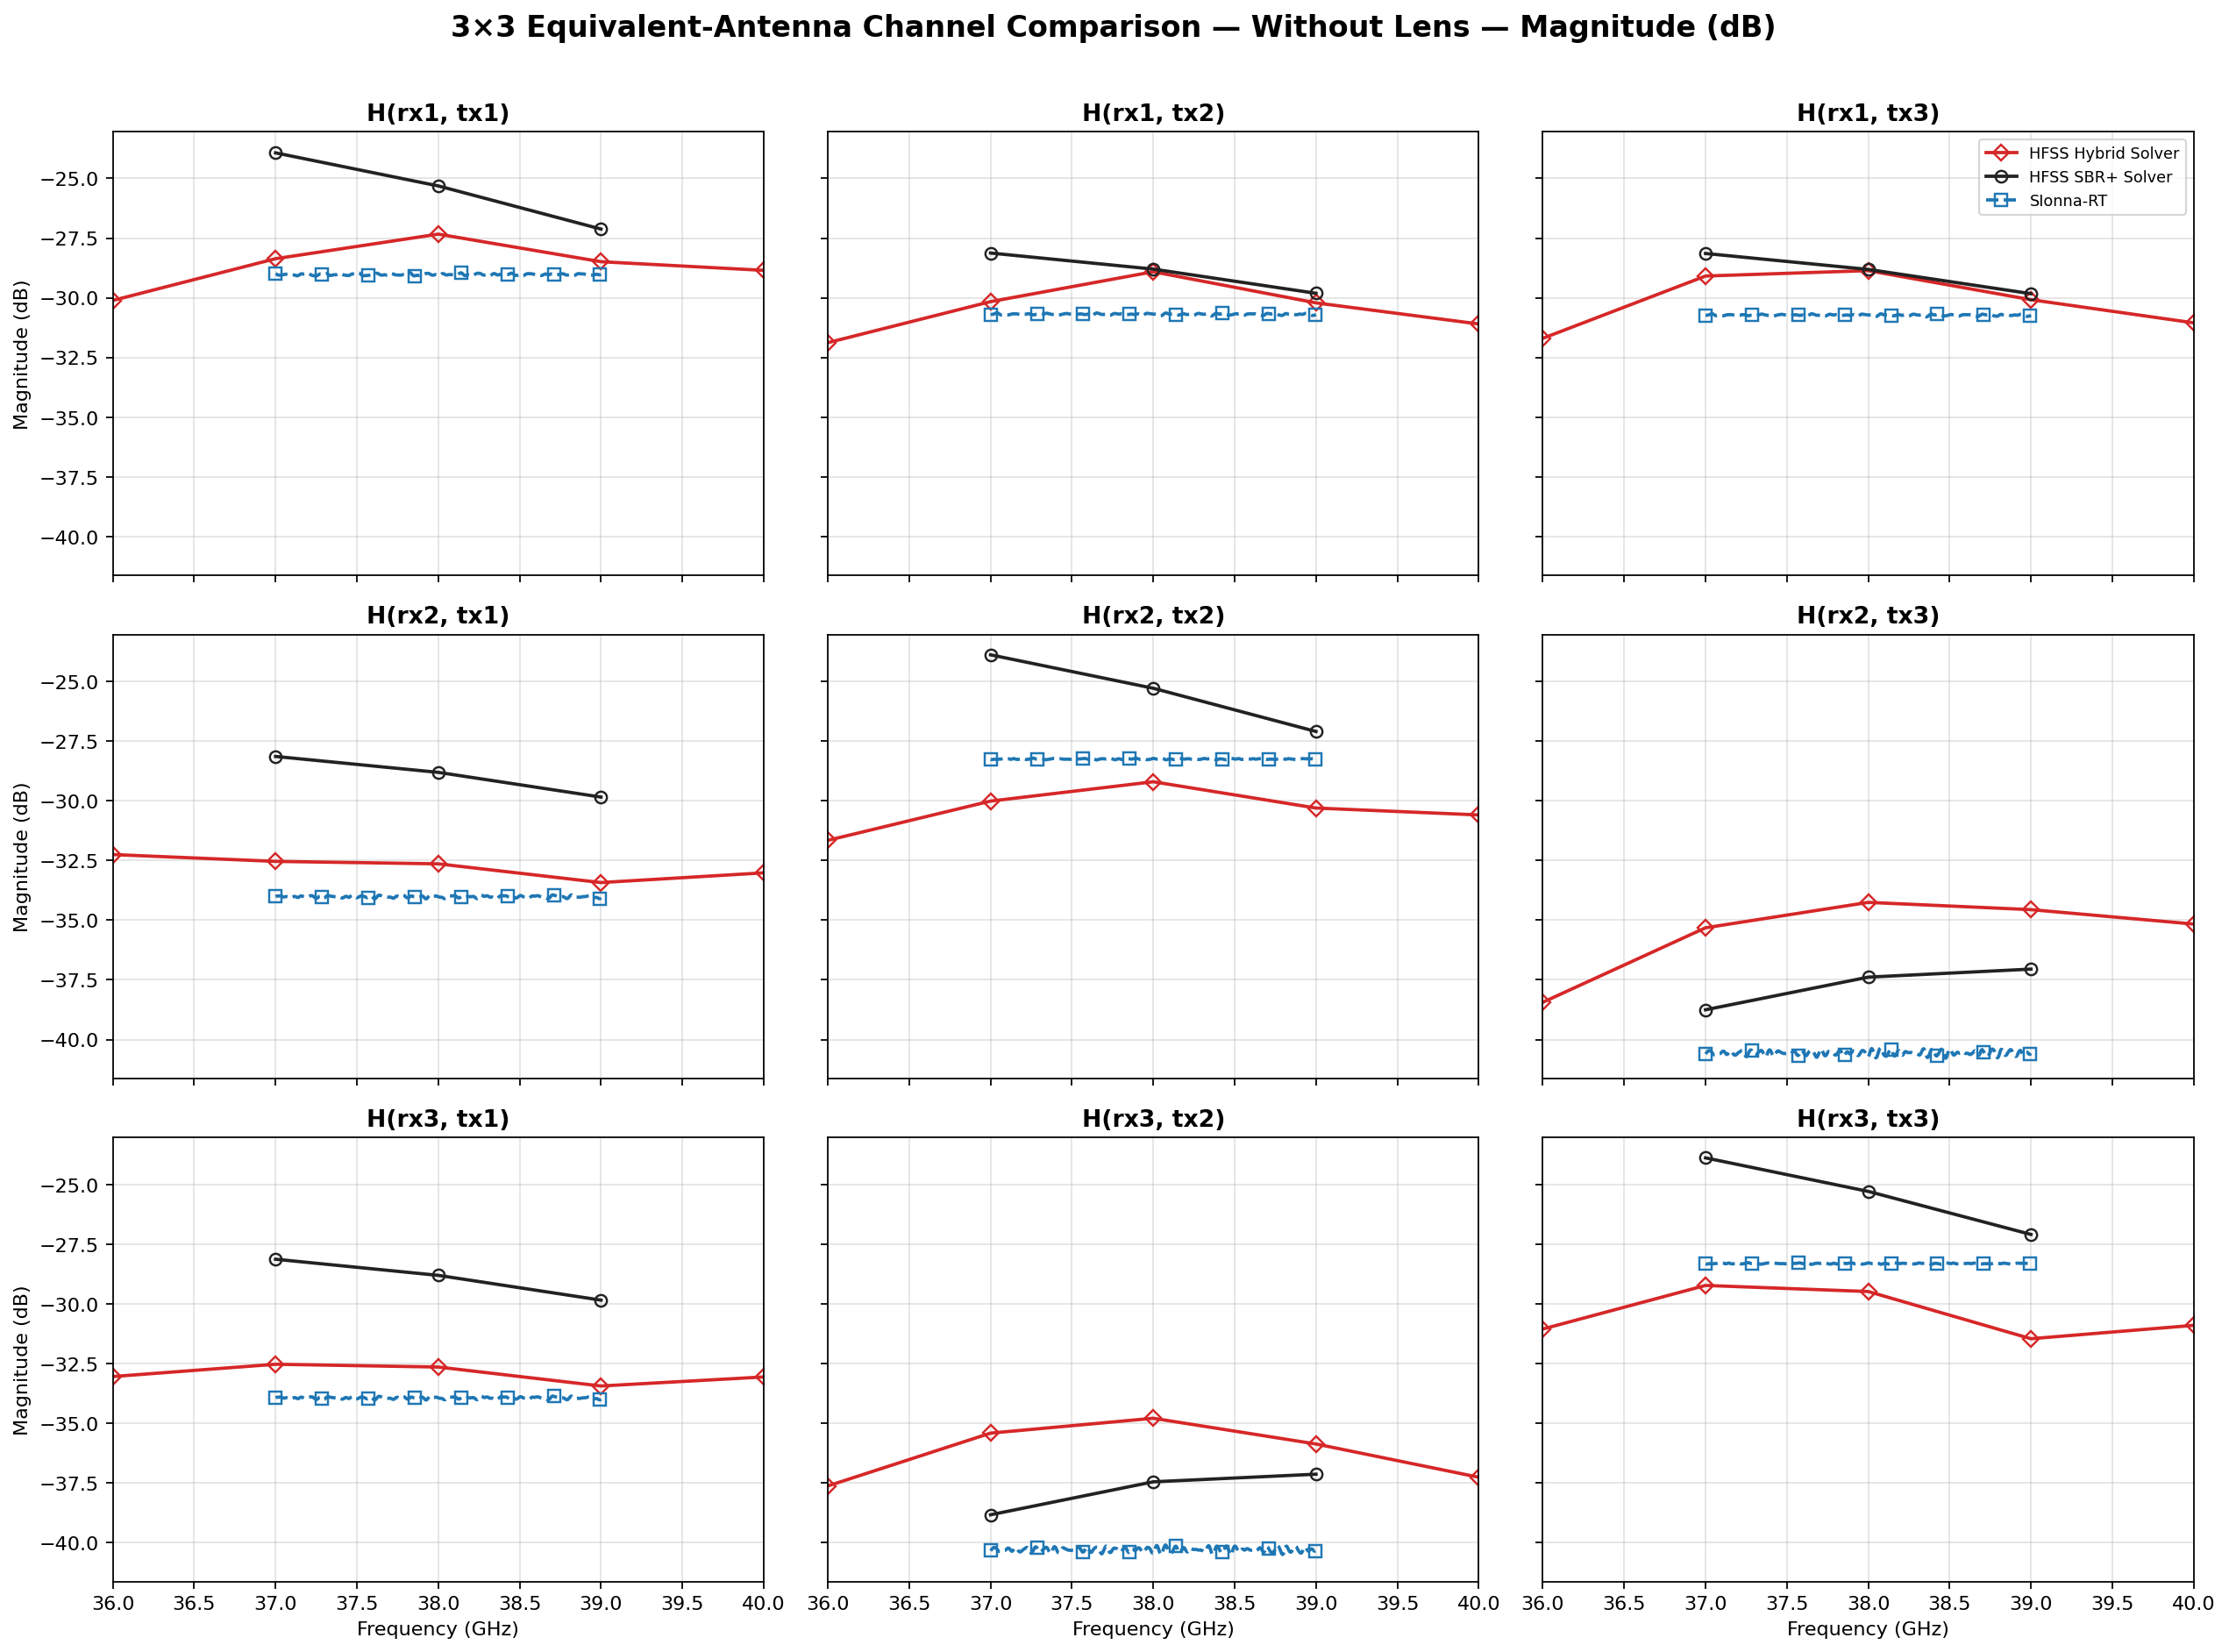
\includegraphics[width=\textwidth]{image/channel_comparison_results/channel_3x3_without_magnitude_db.png}
    \caption{Inter-solver comparison of the $3\times3$ channel magnitudes at
    37, 38, and 39~GHz without the antenna lens.}
    \label{fig:comparison_channel_without_magnitude}
\end{figure}

The pairwise discrepancy summary in
Fig.~\ref{fig:comparison_pairwise_discrepancy} quantifies this observation.
With the lens, SBR+ and Sionna-RT have the smallest mean absolute magnitude
difference, $3.66$~dB, and the smallest centered frequency-shape difference,
$1.46$~dB. Hybrid and Sionna-RT differ by $4.71$~dB in absolute magnitude,
whereas Hybrid and SBR+ differ by $6.11$~dB. Without the lens, Hybrid and
Sionna-RT have the closest magnitude and centered-shape agreement, with mean
differences of $2.20$~dB and $0.49$~dB, respectively. The without-lens Hybrid
and SBR+ solutions provide the closest aligned-phase agreement, with a mean
absolute phase difference of approximately $4.70^\circ$.

\begin{figure}[H]
    \centering
    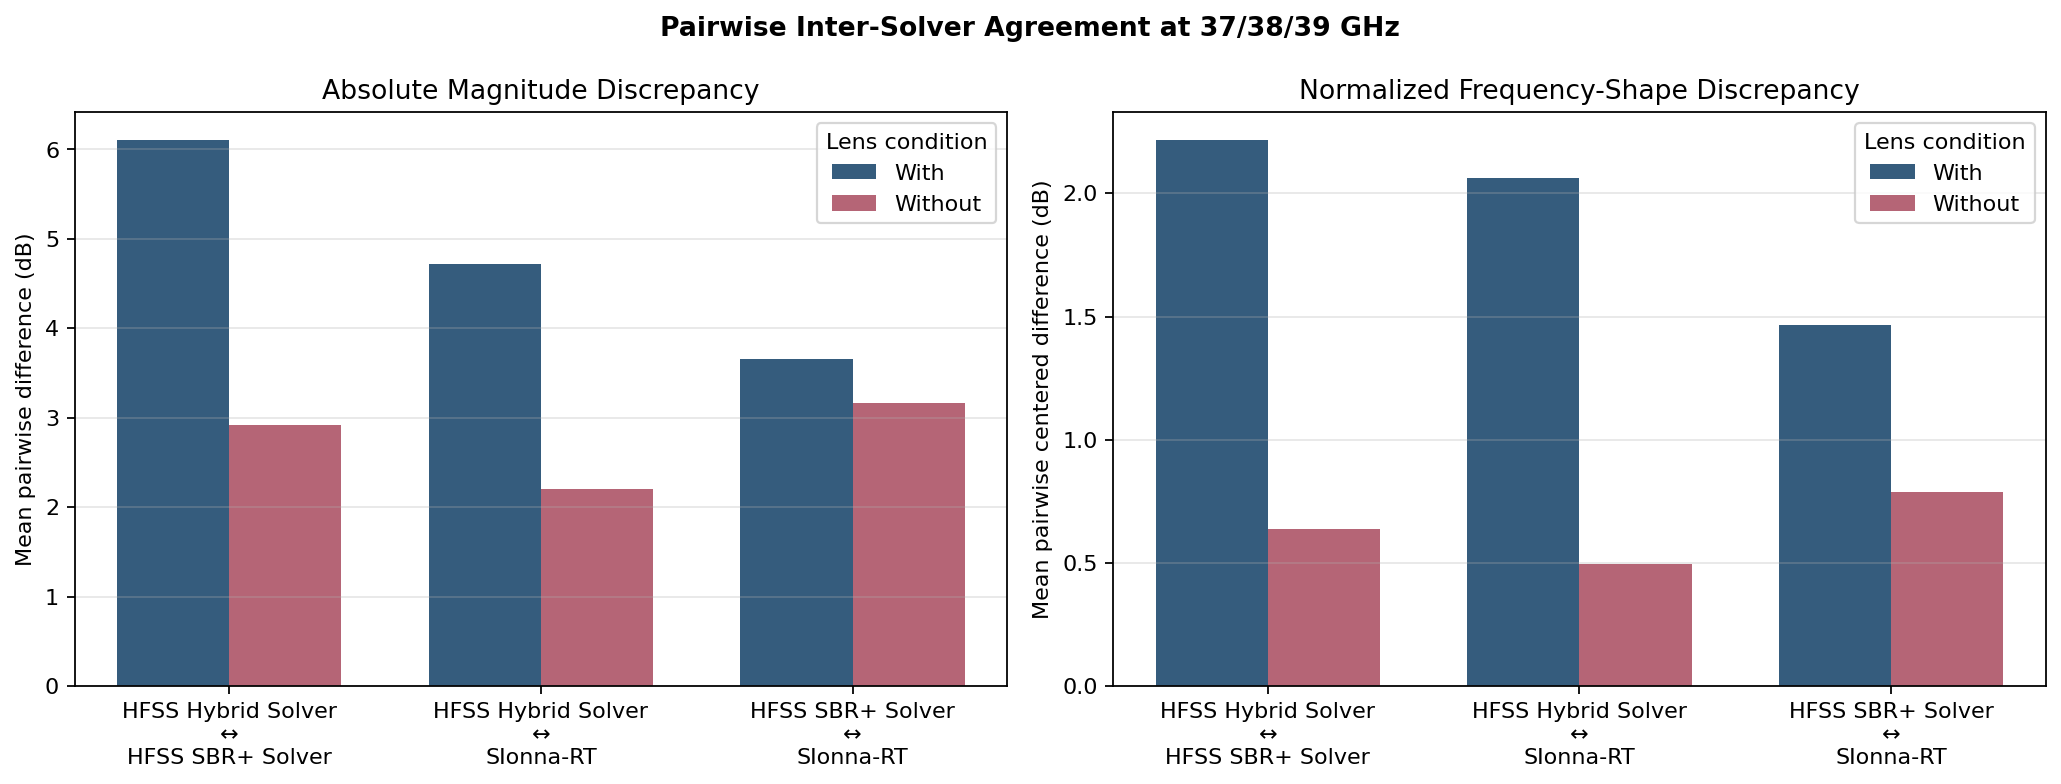
\includegraphics[width=0.92\textwidth]{image/channel_comparison_results/inter_solver_pairwise_discrepancy.png}
    \caption{Mean pairwise absolute-magnitude and centered frequency-shape
    discrepancies among the Hybrid, SBR+, and Sionna-RT solvers. A smaller
    value indicates closer inter-solver agreement.}
    \label{fig:comparison_pairwise_discrepancy}
\end{figure}

\subsection{Lens-Effect Comparison}

The common lens-effect quantity is
\begin{equation}
    \Delta H_{ij,\mathrm{lens}}
    =H_{ij,\mathrm{with,dB}}-H_{ij,\mathrm{without,dB}}.
    \label{eq:comparison_lens_gain}
\end{equation}
Figure~\ref{fig:comparison_lens_gain} shows that all three solvers predict
positive gain for the direction-matched diagonal links and predominantly
negative gain for the off-diagonal links. Averaged over the three anchor
frequencies, the diagonal gains are $8.33$~dB for Hybrid, $5.33$~dB for
SBR+, and $7.12$~dB for Sionna-RT. The corresponding mean off-diagonal
changes are $-7.58$, $-7.86$, and $-7.48$~dB. The Hybrid off-diagonal range
does include a small positive maximum of $0.46$~dB, so cross-coupling
suppression is the dominant trend rather than an exception-free rule.

\begin{figure}[H]
    \centering
    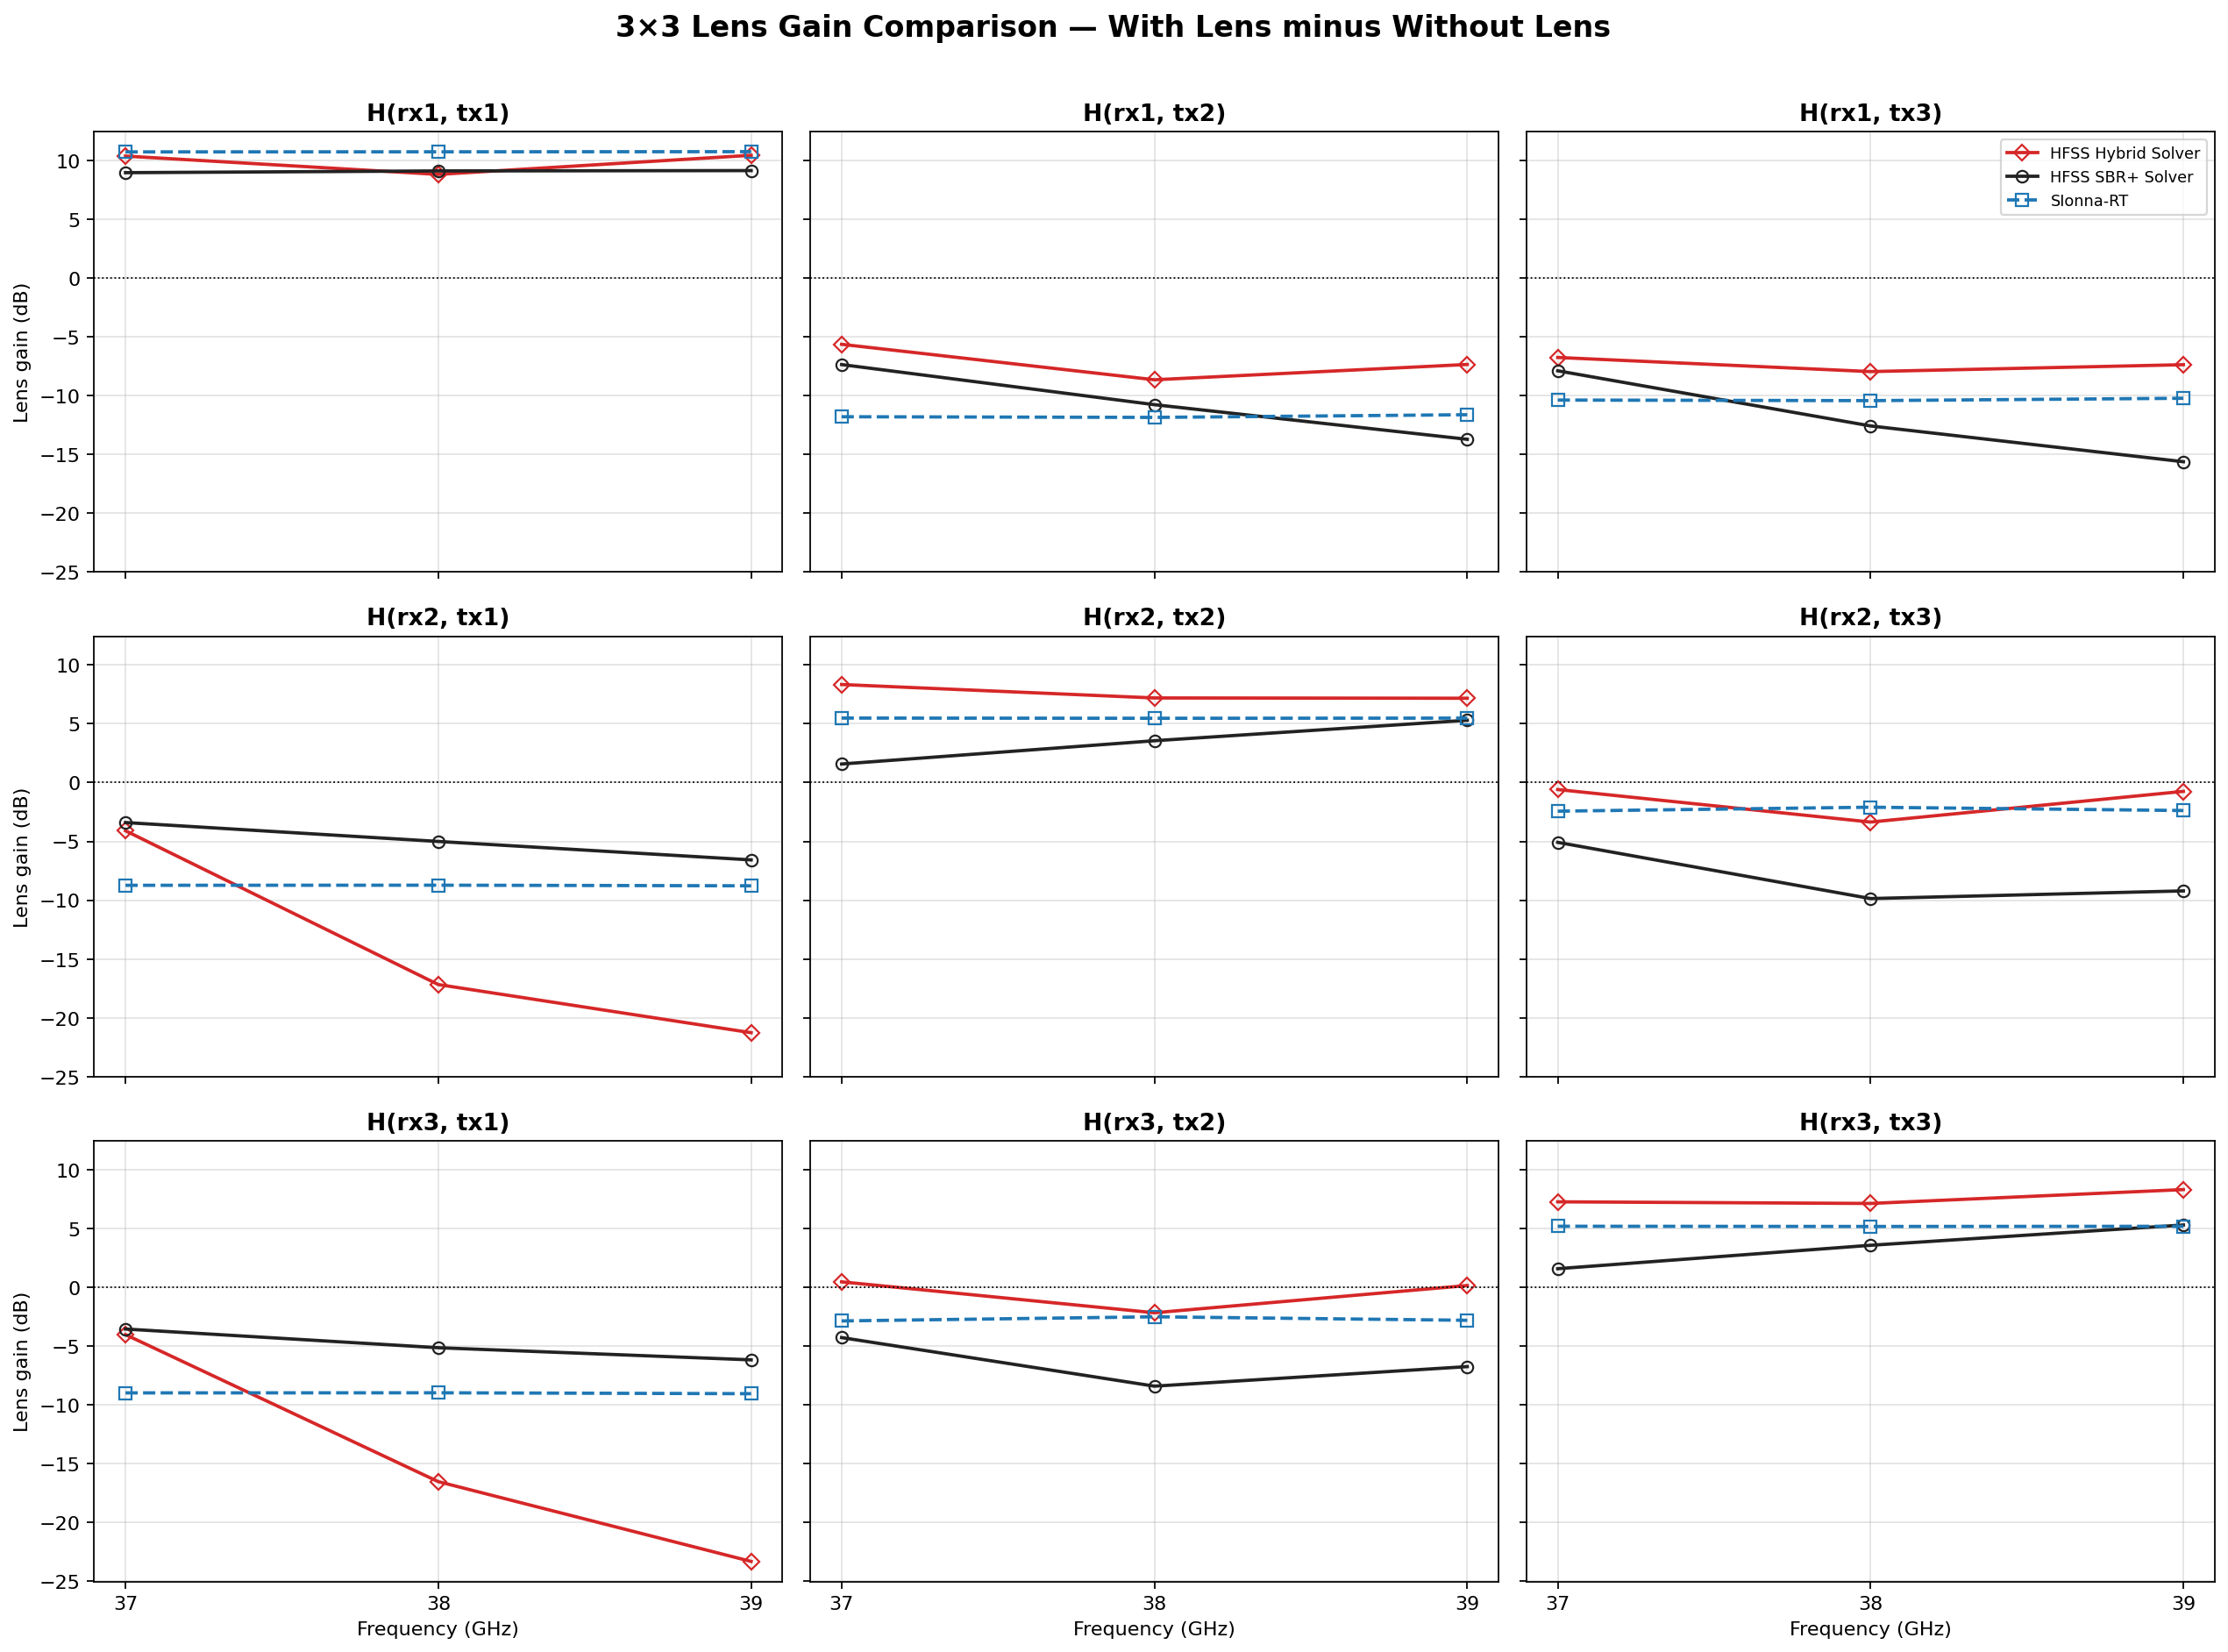
\includegraphics[width=\textwidth]{image/channel_comparison_results/channel_3x3_lens_gain.png}
    \caption{Lens-induced channel-magnitude change for every canonical TX--RX
    pair and solver. Positive values indicate enhancement and negative values
    indicate attenuation after adding the lens.}
    \label{fig:comparison_lens_gain}
\end{figure}

Across the 27 combinations of nine links and three frequencies, the three
solvers unanimously agree on whether the lens increases or decreases the
channel magnitude at 25 points ($92.6\%$). The only non-unanimous cases are
$H(\mathrm{rx}3,\mathrm{tx}2)$ at 37 and 39~GHz, for which two solvers
predict a decrease and one predicts an increase. As summarized in
Fig.~\ref{fig:comparison_lens_direction_agreement}, the lens-effect direction
is therefore highly consistent across solvers, even though its exact
magnitude differs.

\begin{figure}[H]
    \centering
    
\includegraphics[width=0.58\textwidth]{image/channel_comparison_results/lens_effect_direction_agreement.png}
    \caption{Fraction of the 37, 38, and 39~GHz anchor points for which all
    three solvers agree on the direction of the lens-induced change.}
    \label{fig:comparison_lens_direction_agreement}
\end{figure}

\subsection{Inter-Solver MIMO Quality and Capacity}

Figure~\ref{fig:comparison_mimo_raw} compares condition number, effective
rank, and 20-dB capacity while retaining absolute channel gain. A numerical
comparison at the 38-GHz center frequency is given in
Table~\ref{tab:comparison_mimo_38ghz}.

\begin{figure}[H]
    \centering
    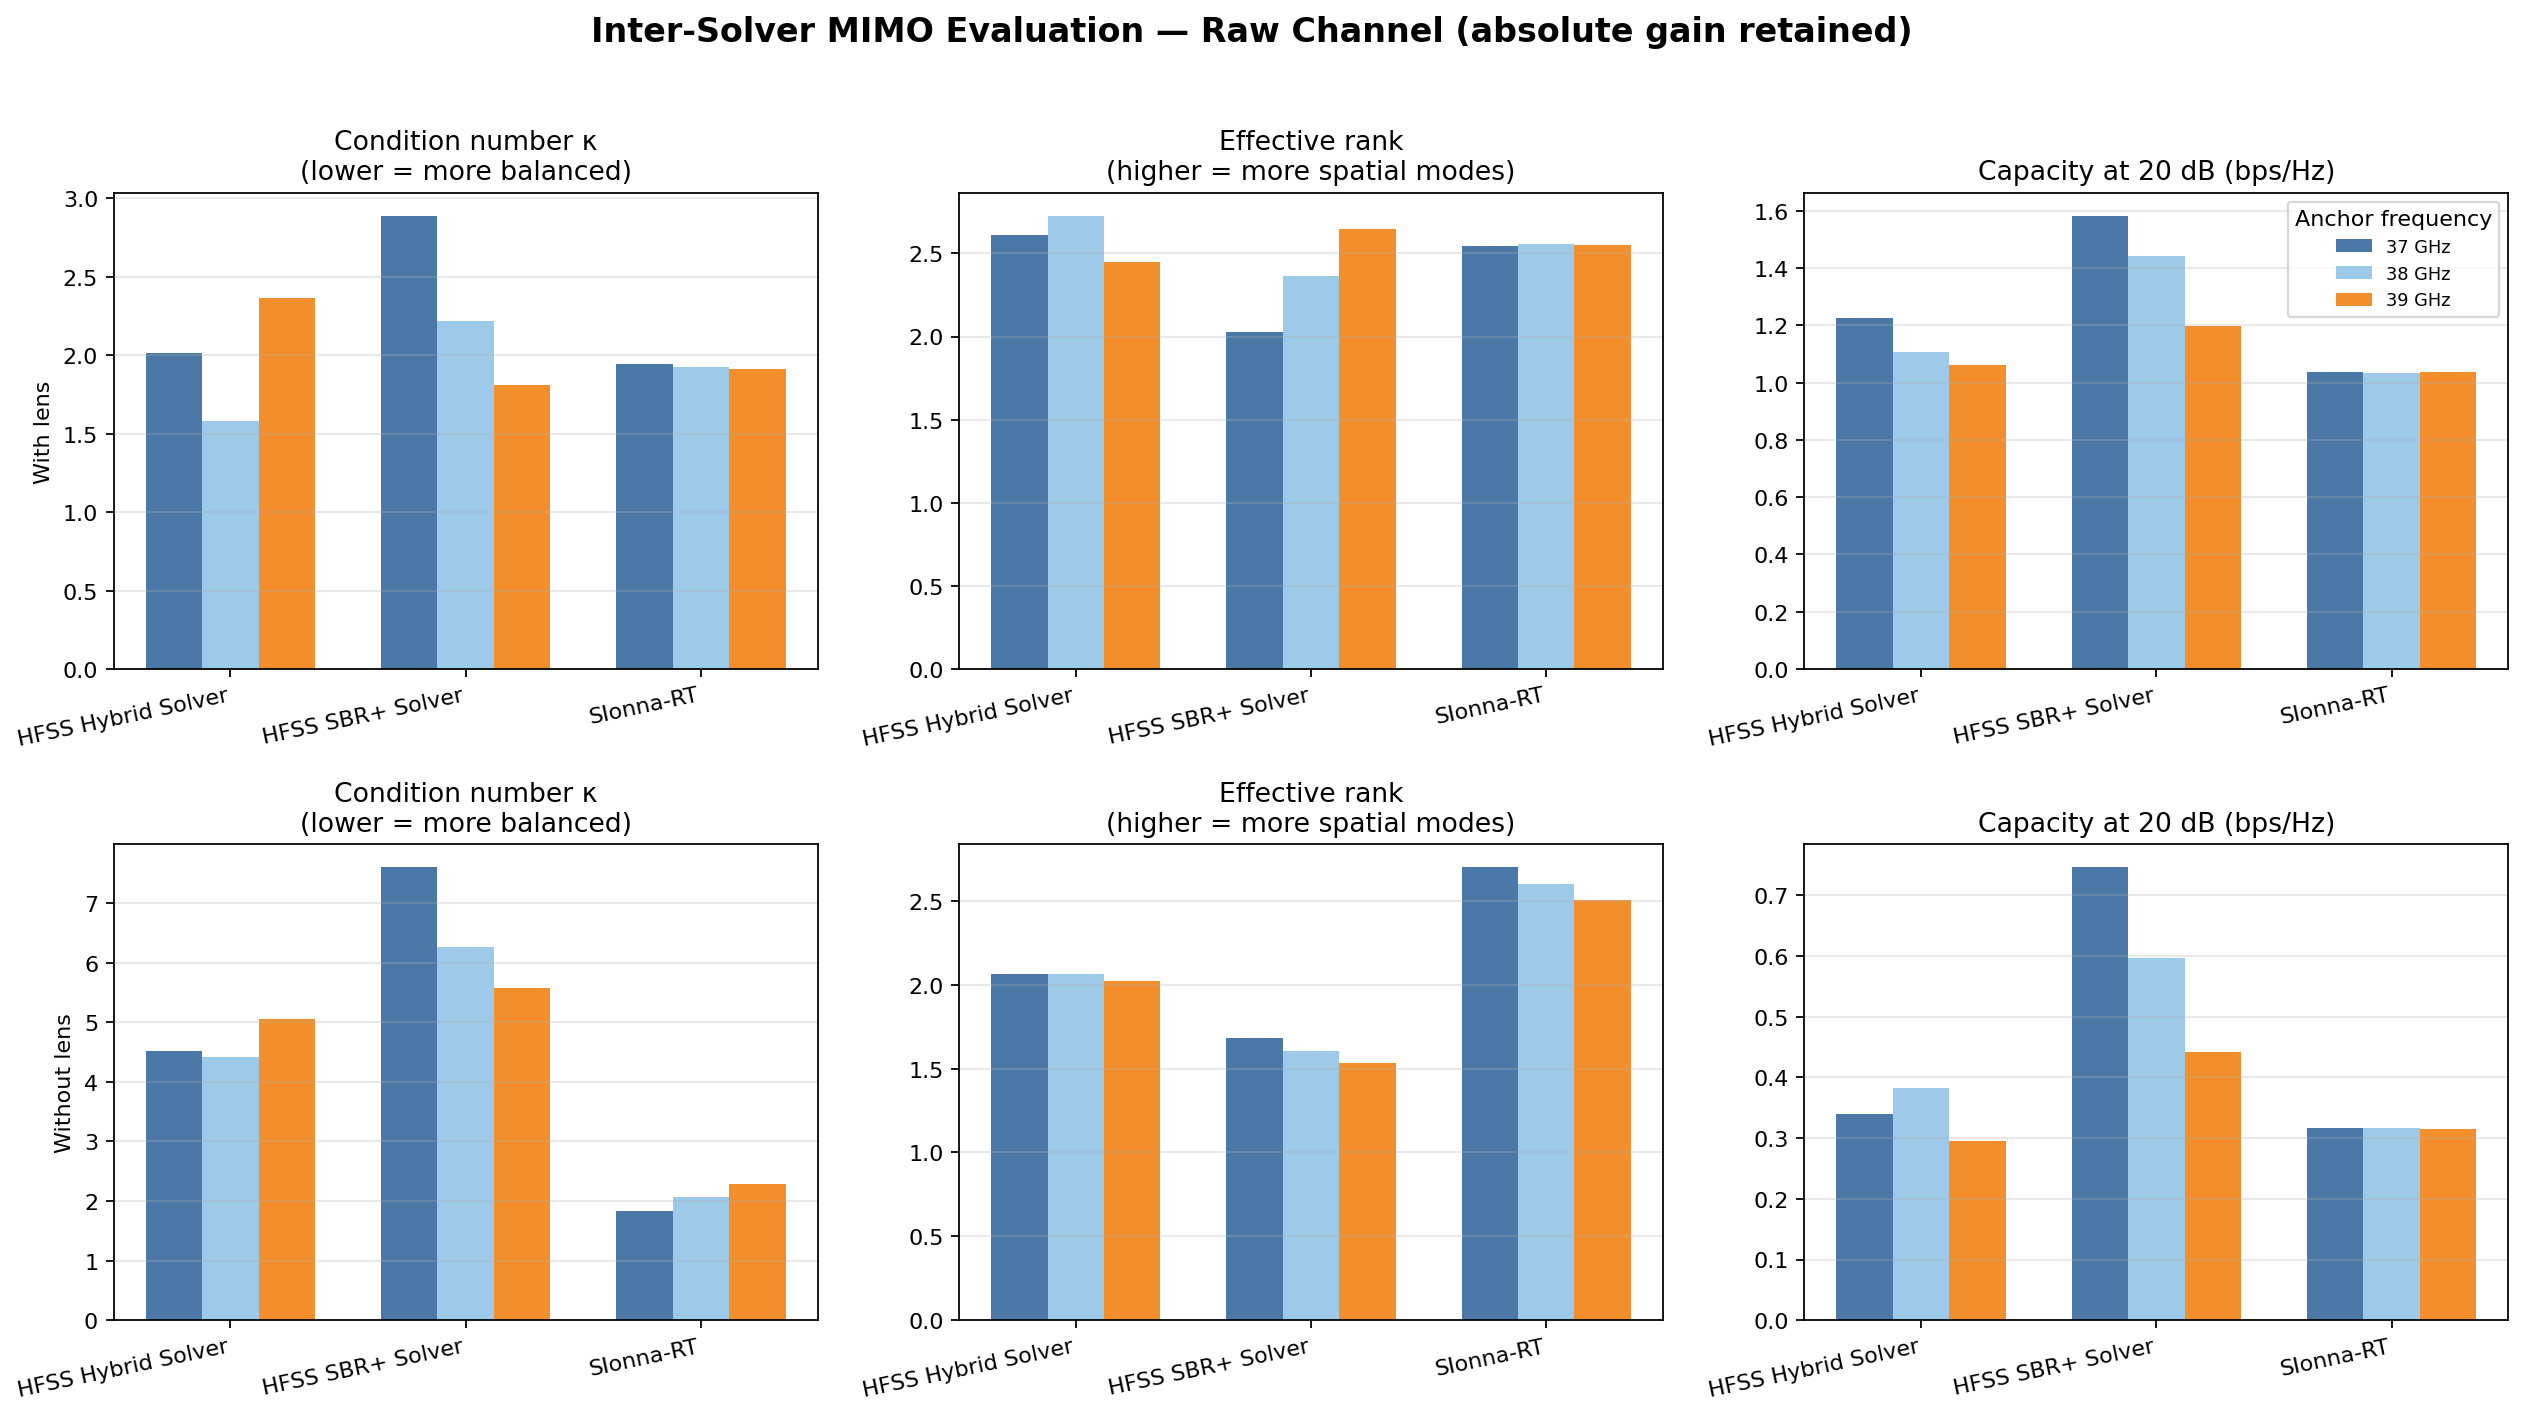
\includegraphics[width=\textwidth]{image/channel_comparison_results/mimo_evaluation_raw.png}
    \caption{Raw-channel inter-solver MIMO evaluation at 37, 38, and 39~GHz.
    The upper row represents the with-lens condition and the lower row the
    without-lens condition.}
    \label{fig:comparison_mimo_raw}
\end{figure}

\begin{table}[H]
    \centering
    \small
    \caption{Raw-channel MIMO metrics at 38~GHz.}
    \label{tab:comparison_mimo_38ghz}
    \begin{tabular}{llccc}
        \hline
        \textbf{Solver} & \textbf{Lens} &
        \textbf{$\kappa$} & \textbf{$r_{\mathrm{eff}}$} &
        \textbf{$C_{20\,\mathrm{dB}}$ (bps/Hz)} \\
        \hline
        Hybrid    & With    & 1.579 & 2.728 & 1.108 \\
        Hybrid    & Without & 4.424 & 2.062 & 0.382 \\
        SBR+      & With    & 2.215 & 2.363 & 1.443 \\
        SBR+      & Without & 6.255 & 1.608 & 0.597 \\
        Sionna-RT & With    & 1.924 & 2.555 & 1.033 \\
        Sionna-RT & Without & 2.064 & 2.604 & 0.317 \\
        \hline
    \end{tabular}
\end{table}

At 38~GHz, all solvers predict a capacity increase after adding the lens.
Hybrid improves from $0.382$ to $1.108$~bps/Hz, SBR+ from $0.597$ to
$1.443$~bps/Hz, and Sionna-RT from $0.317$ to $1.033$~bps/Hz. Hybrid gives
the most balanced with-lens channel at this frequency
($\kappa=1.579$) and the highest effective rank ($2.728$), whereas SBR+
predicts the largest absolute capacity ($1.443$~bps/Hz). Sionna-RT predicts
the smallest change in condition number, but still produces a substantial
capacity increase because its singular values become stronger.

The normalized singular values in
Fig.~\ref{fig:comparison_normalized_singular_values} separate spatial balance
from absolute gain. With the lens, all solvers retain three visible spatial
modes across the anchor frequencies. Without the lens, Hybrid and especially
SBR+ show a relatively weak third normalized singular value, whereas
Sionna-RT predicts a more balanced normalized mode distribution. This
explains why raw capacity rankings should be interpreted together with both
absolute channel strength and normalized spatial structure.

\begin{figure}[H]
    \centering
    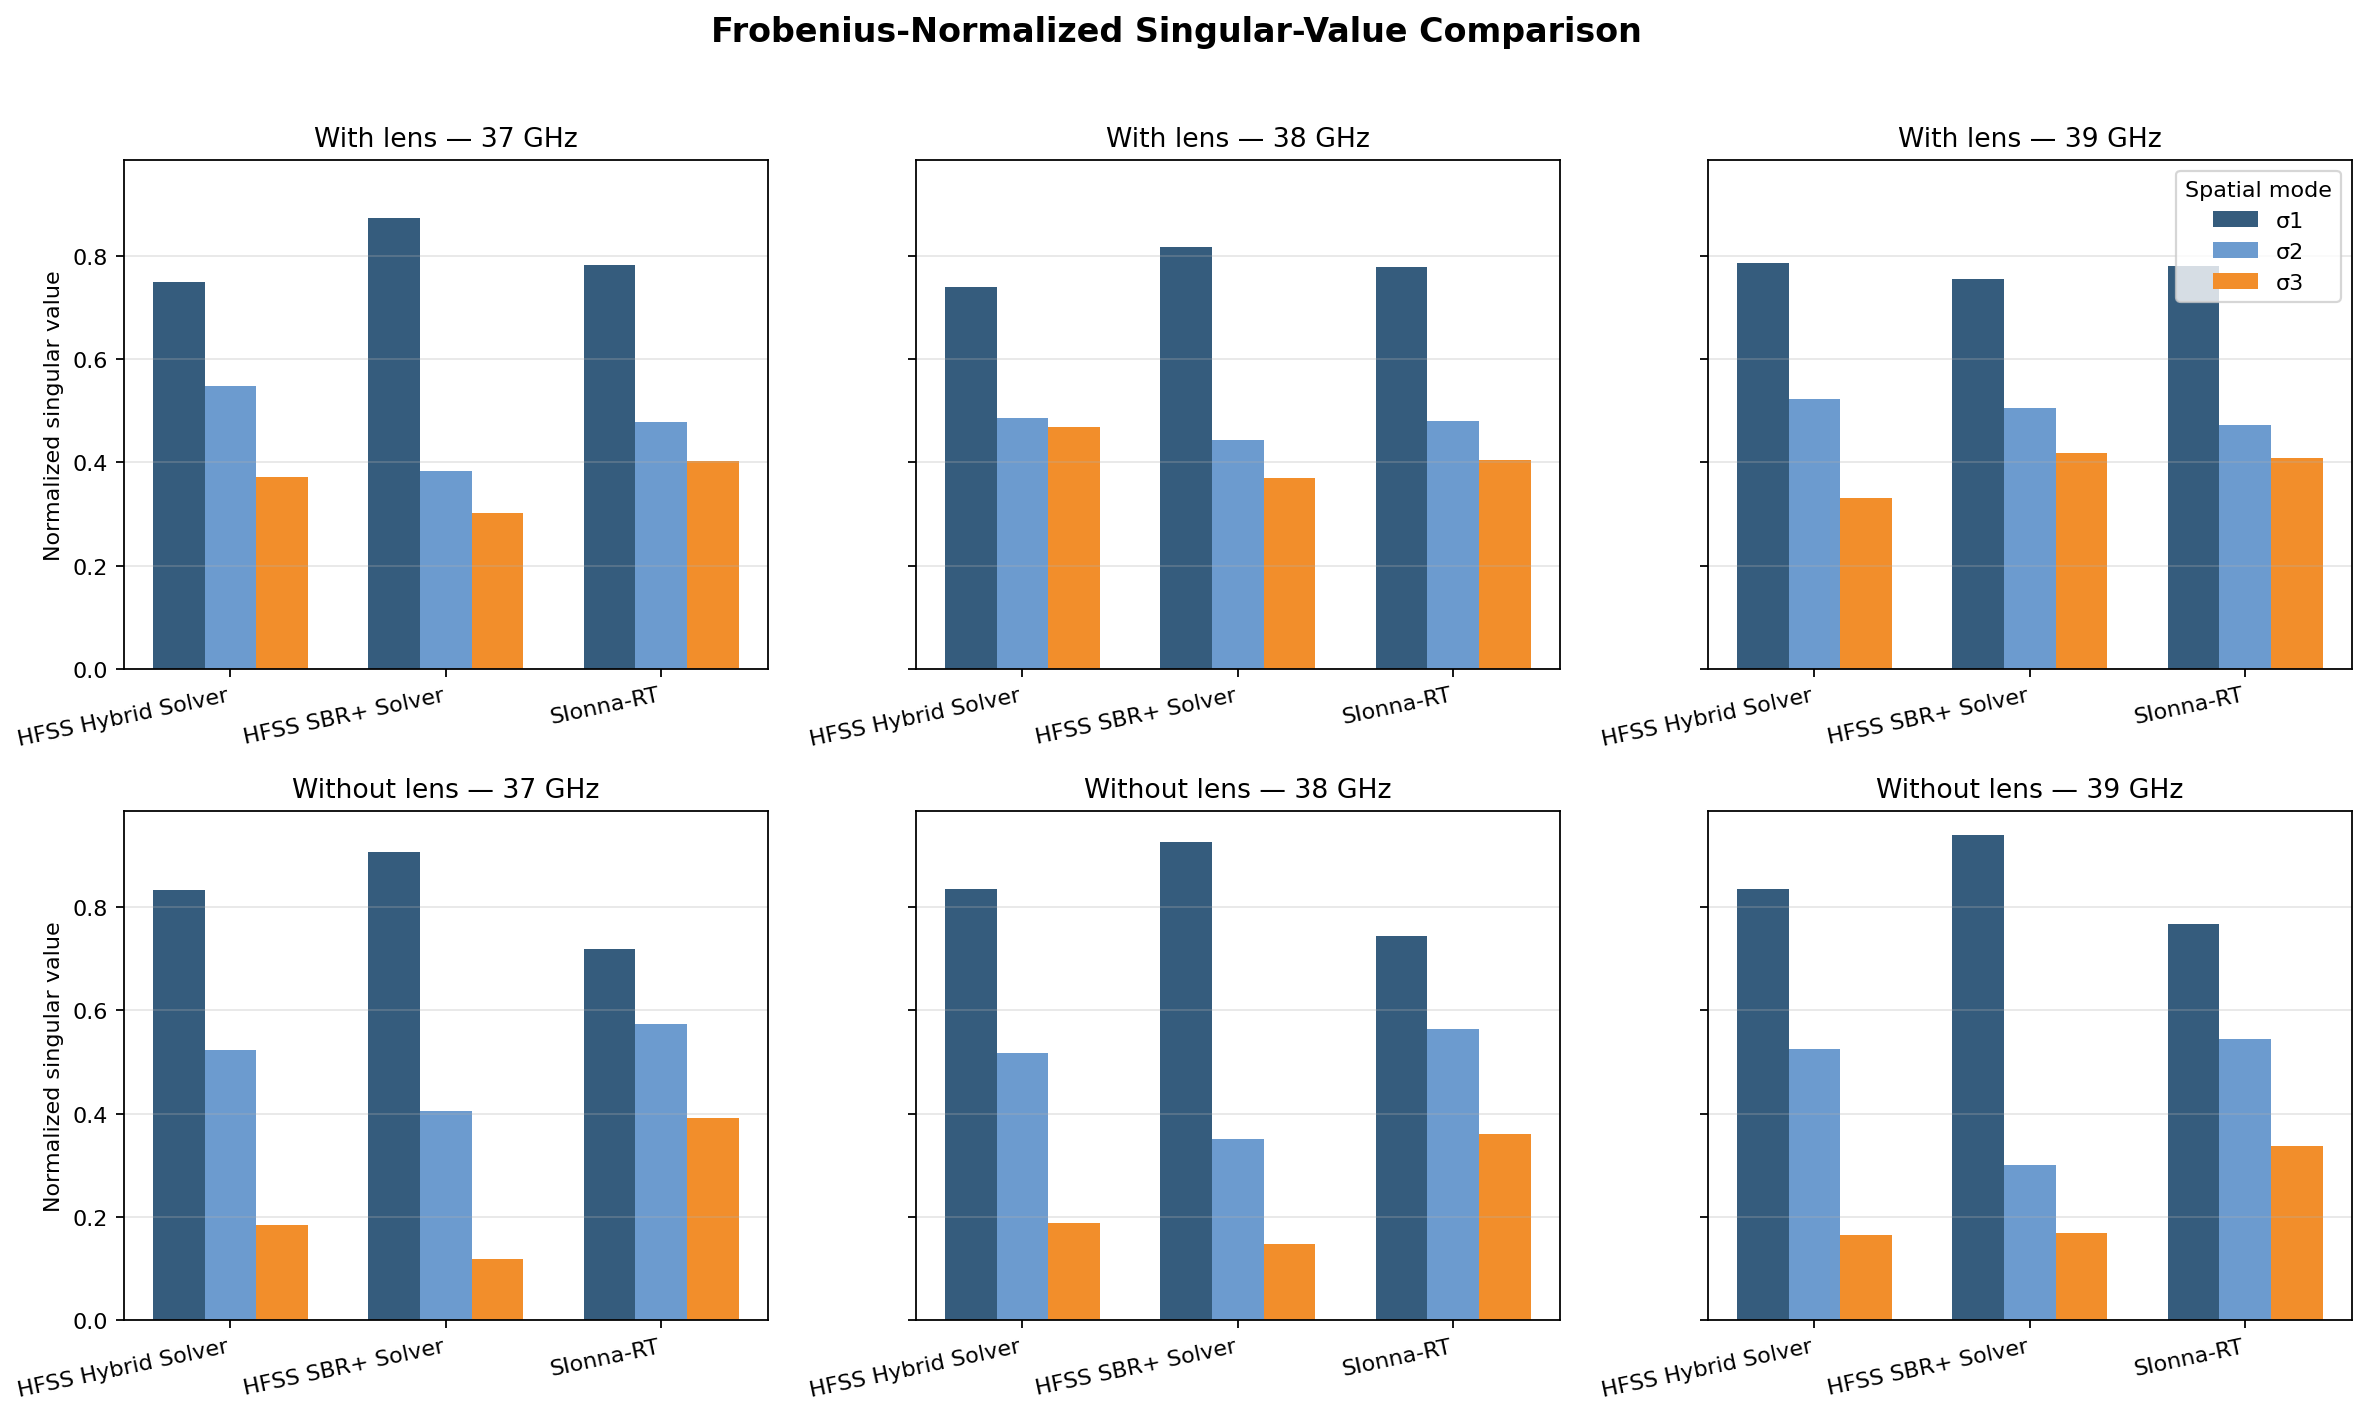
\includegraphics[width=\textwidth]{image/channel_comparison_results/mimo_normalized_singular_values.png}
    \caption{Frobenius-normalized singular values for the three solvers at the
    common anchor frequencies. Normalization removes the absolute-gain
    difference and highlights only the relative spatial-mode structure.}
    \label{fig:comparison_normalized_singular_values}
\end{figure}

\subsection{Spatial-Correlation Comparison}

The spatial-correlation comparison in
Fig.~\ref{fig:comparison_spatial_correlation} provides the most consistent
matrix-level evidence of the lens benefit. At 38~GHz, the mean RX/TX
off-diagonal correlations with the lens are $0.085/0.126$ for Hybrid,
$0.213/0.188$ for SBR+, and $0.177/0.181$ for Sionna-RT. Without the lens,
the corresponding values increase to $0.393/0.561$, $0.767/0.767$, and
$0.297/0.335$. Thus, every solver predicts lower RX- and TX-side spatial
correlation after adding the lens.

\begin{figure}[H]
    \centering
    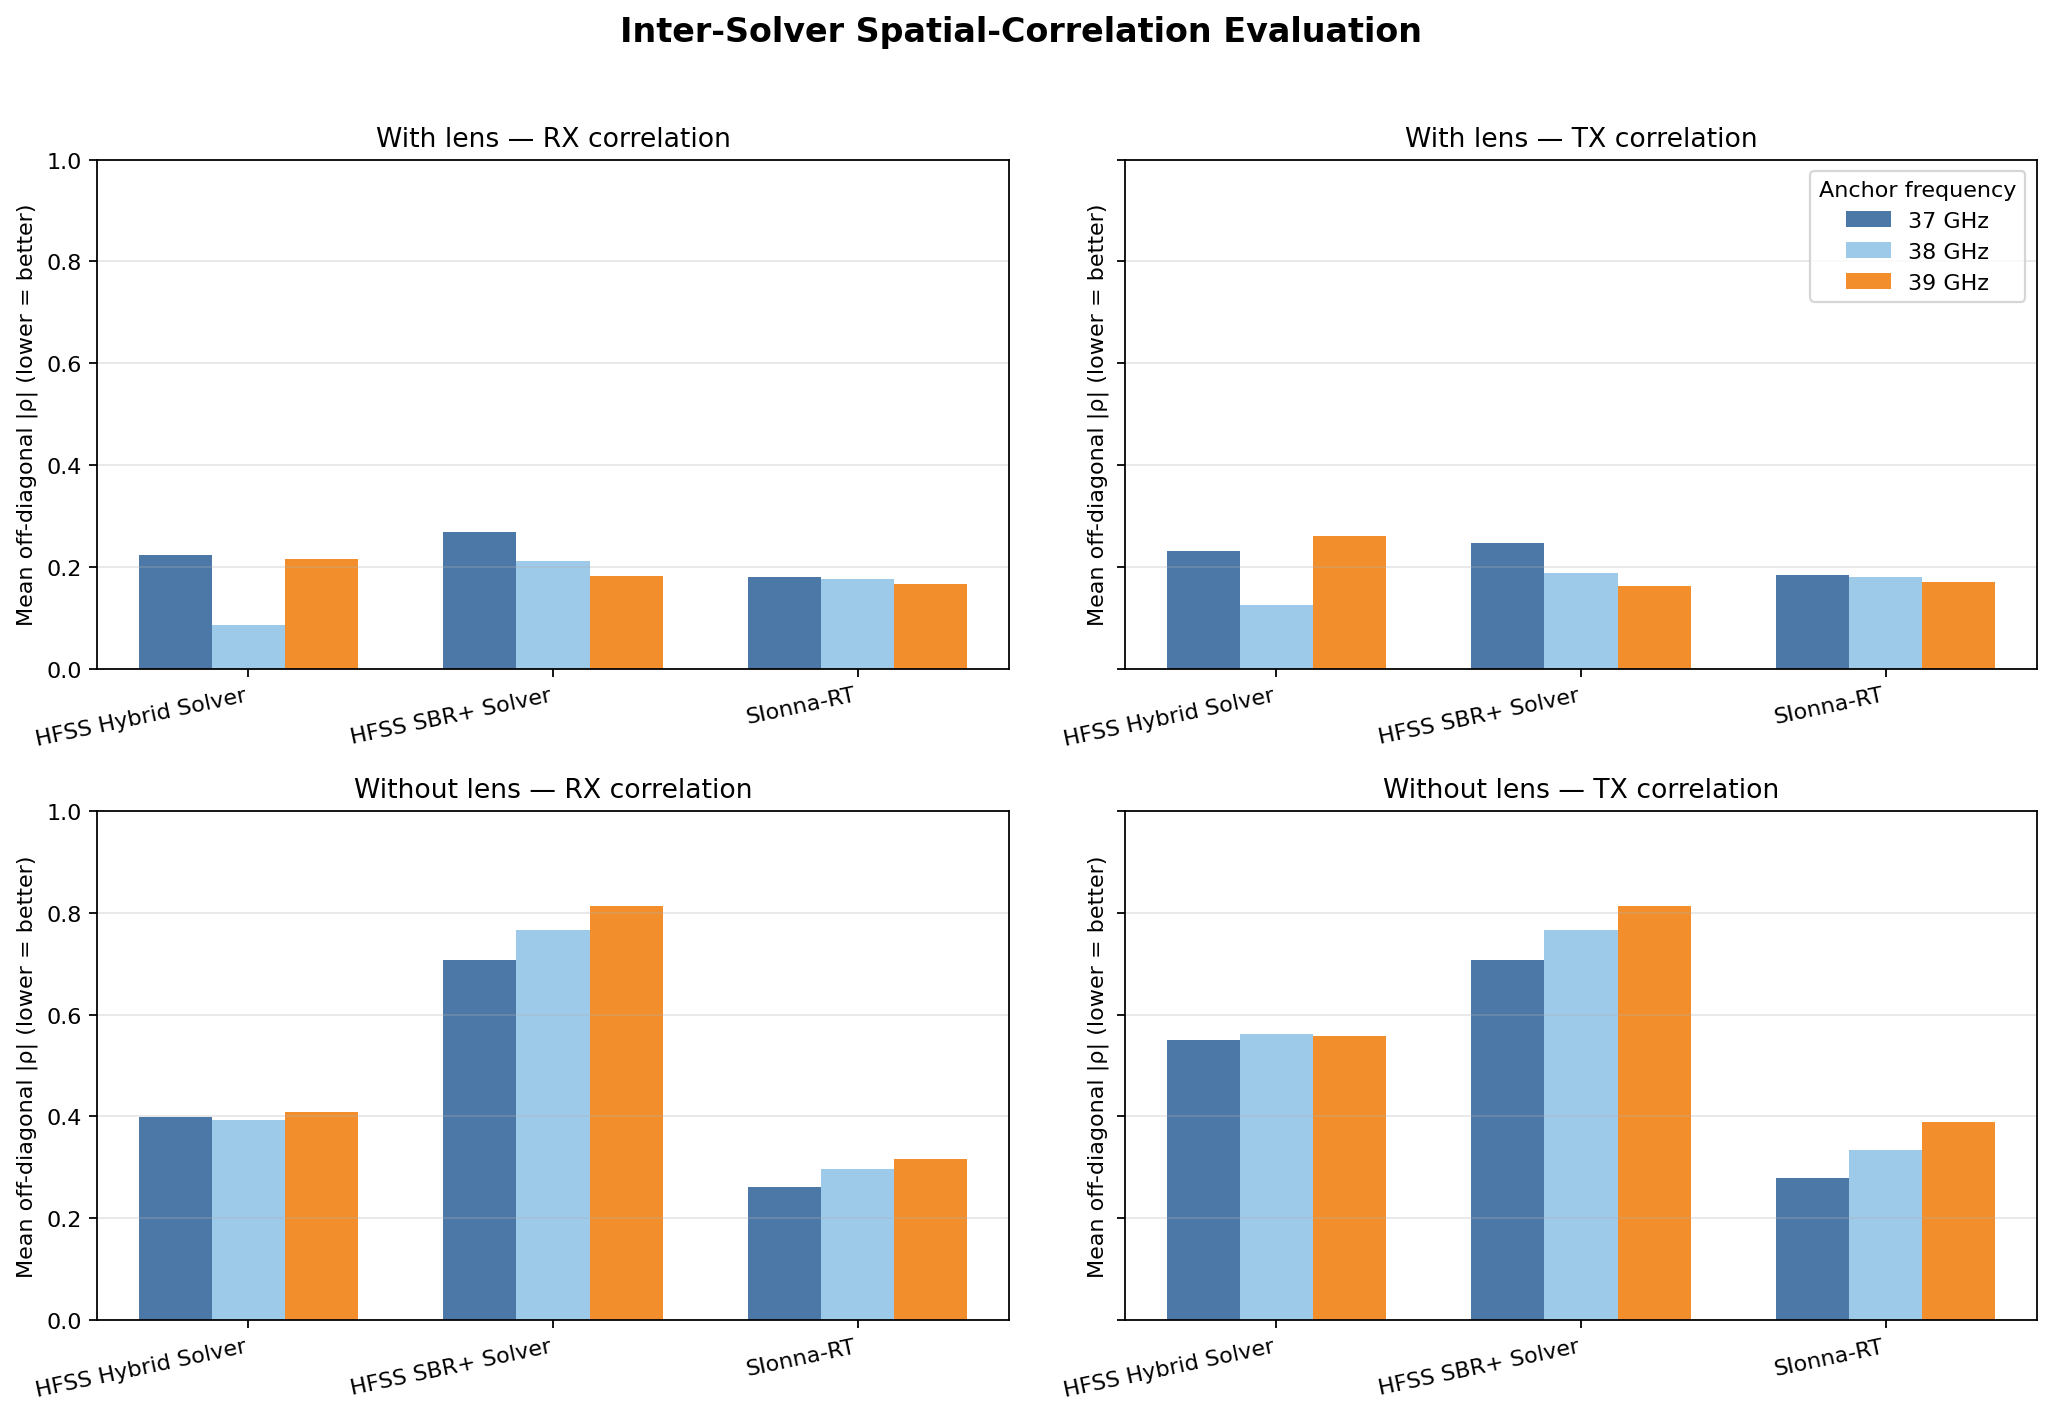
\includegraphics[width=\textwidth]{image/channel_comparison_results/mimo_spatial_correlation_evaluation.png}
    \caption{Mean off-diagonal RX- and TX-side spatial correlation for the
    three solvers at 37, 38, and 39~GHz, with and without the lens. Lower
    values indicate better spatial separation.}
    \label{fig:comparison_spatial_correlation}
\end{figure}

\subsection{Overall Comparison and Interpretation}

The three solvers support the same principal engineering conclusion: the
antenna lens reinforces the intended direction-matched channels, suppresses
most cross-directional coupling, increases the raw 20-dB MIMO capacity, and
reduces spatial correlation. This conclusion is robust because the sign of
the lens effect agrees unanimously for $92.6\%$ of the compared link-frequency
points and all three solvers predict improved capacity and correlation at the
38-GHz center frequency.

The solvers nevertheless should not be treated as numerically
interchangeable. Absolute with-lens magnitude differences remain several
decibels, phase agreement is weaker than magnitude-shape agreement for some
solver pairs, and the predicted condition number and effective rank differ.
SBR+ and Sionna-RT agree most closely on with-lens magnitude, while Hybrid and
Sionna-RT agree most closely without the lens. Hybrid predicts the best
with-lens spatial balance at 38~GHz, SBR+ predicts the highest raw capacity,
and Sionna-RT predicts the most stable full-band behavior. Therefore, the
cross-solver evidence is strongest for qualitative lens trends and relative
MIMO improvement; exact link magnitude and phase should remain
solver-specific unless further reconciled against measurement.


\section{Monte Carlo \texorpdfstring{$9\times9$}{9x9} Antenna Simulation:
Discussion and Conclusions}

\subsection{Technical Summary}

Two notebooks are used to compare a 38-GHz indoor channel in a
$20~\mathrm{m}\times20~\mathrm{m}\times3~\mathrm{m}$ room. The first
configuration does not use a lens and applies the same patch-antenna pattern
to every RX configuration. The second configuration uses a lens and applies
different HFSS far-field patterns for lens angles of $+60^\circ$, $+45^\circ$,
$+30^\circ$, $+15^\circ$, $0^\circ$, $-15^\circ$, $-30^\circ$,
$-45^\circ$, and $-60^\circ$.

Each notebook contains 20 Monte Carlo drops. Every drop consists of nine
randomly positioned transmitters, and the same TX positions are evaluated
against all nine RX configurations. Consequently, each notebook contains 180
drop--RX results. This paired design provides a fair comparison between lens
angles and between the lens and no-lens cases because every pair uses
identical TX geometry.

The aggregate results indicate that the lens increases the median capacity
from $7.29$ to $7.67$~bit/s/Hz and the median ideal throughput from $2.92$ to
$3.07$~Gbit/s. The benefit is not uniform over direction: intermediate
negative angles, particularly $-30^\circ$, provide the highest median
performance, whereas $+60^\circ$ performs worse than the no-lens antenna.
Because only 20 drops and 100,000 path samples per source are used, these
results should be considered preliminary.

\subsection{Simulation Sources and Scope}

The simulation sources are:
\small
\begin{itemize}
    \item No-lens notebook:
    \path{Setup_20mx20m_wolens_9x9_Patch_randomCom.ipynb}. It uses
    \path{FarFieldData_Patch_38GHz.csv} for all angle labels.
    \item Lens notebook:
    \path{Setup_20mx20m_lens_9x9_Patch_randomCom.ipynb}. It uses the HFSS
    far-field patterns associated with the configured lens angles.
\end{itemize}
\normalsize
This discussion evaluates the Monte Carlo outputs already stored in the
notebooks; the notebooks were not re-executed.

\begin{table}[H]
    \centering
    \caption{Scope and parameters of the Monte Carlo $9\times9$ simulation.}
    \label{tab:monte_carlo_scope}
    \small
    \begin{tabular}{ll}
        \hline
        \textbf{Parameter} & \textbf{Value} \\
        \hline
        Room dimensions & $20~\mathrm{m}\times20~\mathrm{m}\times3~\mathrm{m}$ \\
        Carrier frequency / bandwidth & 38~GHz / 400~MHz \\
        Frequency points & 401 \\
        Monte Carlo drops / TXs per drop & 20 / 9 \\
        RX configurations / results per notebook & 9 / 180 \\
        Random seed & 20260718 \\
        TX height / minimum TX--RX distance & 1.0--2.5~m / 1.0~m \\
        Wall margin / path samples per source & 0.75~m / 100,000 \\
        Power per TX & 10~dBm \\
        Noise figure / noise temperature & 7~dB / 290~K \\
        Capacity-outage threshold & 1~bit/s/Hz \\
        \hline
    \end{tabular}
\end{table}

The 20 drops produce 180 TX points whose stored coordinates span
$-9.24$--$9.19$~m on both the $x$- and $y$-axes and $1.01$--$2.50$~m on the
$z$-axis. The TX--RX distance has a minimum of $1.22$~m, a mean of
$10.56$~m, and a maximum of $19.57$~m. This coverage is consistent with the
sampling constraints and spans a broad portion of the room.

\subsection{Calculation Methodology}

\subsubsection{Channel Generation and Metrics}

For each drop, nine TXs are placed at random positions and pointed toward the
RX. All RX configurations are then tested using the same TX positions, and
the wideband response is evaluated at 401 frequency points. Although the
notebook filenames contain \texttt{Patch}, the Monte Carlo section explicitly
sets the TX pattern to isotropic (\texttt{iso}). Channel variation is
therefore primarily caused by TX position, room propagation, and the RX
pattern rather than TX patch directivity.

The powers from the nine transmitters are combined non-coherently:
\begin{equation}
    P_{\mathrm{RX}}(f)
    =P_{\mathrm{TX}}\sum_{i=1}^{9}\left|H_i(f)\right|^2.
    \label{eq:monte_carlo_rx_power}
\end{equation}
Noise is calculated from $kTB$ and the configured noise figure. The
equivalent SISO spectral efficiency is
\begin{equation}
    C=\mathbb{E}_{f}\!\left[\log_2\left(1+\mathrm{SNR}(f)\right)\right].
    \label{eq:monte_carlo_siso_capacity}
\end{equation}
The reported throughput is the ideal value $B C$, not protocol-level
throughput. RMS delay spread is obtained from the power-delay profile after
applying an IFFT to the channel response.

\subsubsection{Virtual MIMO Evaluation}

The nine RX channels associated with the different angles are combined into
a virtual $9\times9$ MIMO matrix to calculate condition number, effective
rank, and capacity at an SNR of 10~dB. These nine RX measurements do not occur
simultaneously at one physical receiver. The results are therefore indicators
of virtual channel diversity and conditioning and must not be interpreted as
capacity directly achievable by a physical single-antenna RX.

\subsection{Aggregate Lens and No-Lens Results}

\begin{table}[H]
    \centering
    \caption{Aggregate Monte Carlo results with and without the lens.}
    \label{tab:monte_carlo_aggregate}
    \small
    \begin{tabular}{lccc}
        \hline
        \textbf{Metric} & \textbf{Without lens} & \textbf{With lens} &
        \textbf{Change} \\
        \hline
        Median capacity (bit/s/Hz) & 7.29 & 7.67 & $+0.38$ ($+5.2\%$) \\
        5th-percentile capacity (bit/s/Hz) & 6.48 & 5.02 & $-1.46$ \\
        95th-percentile capacity (bit/s/Hz) & 9.21 & 9.68 & $+0.47$ \\
        Median ideal throughput (Gbit/s) & 2.92 & 3.07 & $+0.15$ ($+5.1\%$) \\
        Median RMS delay spread (ns) & 68.29 & 65.01 & $-3.28$ ($-4.8\%$) \\
        Outage below 1 bit/s/Hz & 0.0\% & 0.0\% & No change \\
        \hline
    \end{tabular}
\end{table}

Table~\ref{tab:monte_carlo_aggregate} shows that the lens improves typical
performance and the upper end of the distribution but degrades the 5th
percentile. The capacity range is also wider with the lens. Thus, the lens
provides greater gain in favorable directions while increasing sensitivity
to angle and configuration; the no-lens antenna produces more uniform
performance. The 1-bit/s/Hz outage threshold cannot distinguish the two
configurations because all 360 results exceed it. Thresholds of 5, 6, and
7~bit/s/Hz would provide a more meaningful reliability comparison.

\subsection{Comparison by RX Angle}

\begin{table}[H]
    \centering
    \caption{Median capacity by RX angle in bit/s/Hz.}
    \label{tab:monte_carlo_angle_capacity}
    \small
    \begin{tabular}{rrrr}
        \hline
        \textbf{Angle} & \textbf{Without lens} & \textbf{With lens} &
        \textbf{Difference} \\
        \hline
        $+60^\circ$ & 7.31 & 6.70 & $-0.61$ \\
        $+45^\circ$ & 7.31 & 7.49 & $+0.18$ \\
        $+30^\circ$ & 7.31 & 7.29 & $-0.01$ \\
        $+15^\circ$ & 7.30 & 8.02 & $+0.72$ \\
        $0^\circ$   & 7.30 & 7.68 & $+0.39$ \\
        $-15^\circ$ & 7.29 & 8.28 & $+0.99$ \\
        $-30^\circ$ & 7.29 & \textbf{8.32} & $\mathbf{+1.03}$ \\
        $-45^\circ$ & 7.29 & 8.13 & $+0.84$ \\
        $-60^\circ$ & 7.29 & 7.43 & $+0.14$ \\
        \hline
    \end{tabular}
\end{table}

Without the lens, the median capacity across all angle labels varies by only
approximately $0.02$~bit/s/Hz because every configuration uses the same
patch RX pattern and the RX positions differ by only a few centimeters. With
the lens, the median ranges from $6.70$ to $8.32$~bit/s/Hz, making the RX
angular pattern a major factor. The best result occurs at $-30^\circ$,
followed by $-15^\circ$ and $-45^\circ$, whereas $+60^\circ$ is the weakest
configuration.

The positive/negative-angle asymmetry means that performance cannot be
assumed symmetric based only on angle magnitude. Possible causes include the
far-field patterns, RX orientation, HFSS data mapping, parameter filtering,
and interaction between the antenna pattern and the room geometry.

\subsection{Paired Checks by Drop}

The logged results provide 180 ``with lens minus without lens'' pairs with
identical TX positions. Because the logged values are rounded, they are most
useful for checking the direction of the effect. The median and mean capacity
differences are $+0.40$ and $+0.15$~bit/s/Hz, respectively. The lens produces
higher capacity in 106 of the 180 pairs ($58.9\%$), while the median SNR
difference is $+1.3$~dB and the median RMS-delay-spread difference is
$-4.70$~ns.

By angle, the lens performs better in 15 of 20 drops at both $+15^\circ$ and
$-15^\circ$, in 14 of 20 drops at both $0^\circ$ and $-30^\circ$, and in 13
of 20 drops at $-45^\circ$. At $+60^\circ$, it performs better in only 8 of
20 drops. These paired checks reinforce the conclusion that the benefit
depends on angular alignment and is not universal.

\subsection{Virtual MIMO Channel Conditioning}

\begin{table}[H]
    \centering
    \caption{Virtual $9\times9$ MIMO channel metrics.}
    \label{tab:monte_carlo_virtual_mimo}
    \small
    \begin{tabular}{lcc}
        \hline
        \textbf{Metric} & \textbf{Without lens} & \textbf{With lens} \\
        \hline
        Median condition number & 49.4 (33.8~dB) & 54.0 (34.6~dB) \\
        5th--95th percentile condition-number range & 27.8--44.4~dB &
        29.4--40.6~dB \\
        Median effective rank & 4.09 of 9 & 4.07 of 9 \\
        Median capacity at 10~dB & 21.72~bit/s/Hz & 21.11~bit/s/Hz \\
        \hline
    \end{tabular}
\end{table}

The lens does not improve virtual MIMO conditioning in this configuration.
Its median condition number increases slightly, its effective rank is almost
unchanged, and its median 10-dB capacity decreases by approximately
$0.61$~bit/s/Hz. An effective rank near four further indicates that the nine
angular channels do not provide nine independent spatial modes. This result
does not conflict with the aggregate SISO-capacity improvement: a lens can
increase power at selected angles without improving channel orthogonality.

\subsection{Limitations and Uncertainty}

\begin{enumerate}
    \item Only 20 drops are available, which is insufficient for stable
    distribution-tail and outage estimates.
    \item The stored results use 100,000 path samples per source rather than
    the recommended final setting of 1,000,000.
    \item The Monte Carlo TX pattern is isotropic, so the results do not
    include TX patch-pattern effects.
    \item Every TX radiates 10~dBm. For a fixed total power budget, the
    per-TX power should be reduced by
    $10\log_{10}(9)\approx9.54$~dB.
    \item Capacity is an ideal Shannon bound and excludes modulation,
    practical coding, overhead, interference, channel estimation, and RF
    implementation losses.
    \item Every no-lens angle label uses the same patch CSV; those labels are
    matching identifiers rather than different angular patterns.
    \item RX orientation and HFSS parameter filtering differ for some lens
    angles. Angle signs and positive/negative HFSS-file mapping must be
    verified before the observed asymmetry is treated as physical.
    \item The $9\times9$ MIMO construction is virtual because the nine RX
    states are not measured simultaneously.
    \item An LLVM JIT initialization warning occurs near the start of the
    notebook outputs, although the stored Monte Carlo outputs are complete.
    Execution stability and backend consistency should be checked during
    reproduction.
\end{enumerate}

Given these limitations, the results are appropriate to share with caveats
but should not yet be treated as a final general result.

\subsection{Recommended Follow-Up Simulations}

\begin{enumerate}
    \item Increase the experiment to at least 100--500 drops and use
    1,000,000 path samples per source.
    \item Export full-precision results to CSV or Parquet and calculate
    bootstrap confidence intervals for the paired capacity difference at
    every angle.
    \item Report outage at more demanding thresholds such as 5, 6, and
    7~bit/s/Hz.
    \item Repeat the comparison under a fixed total power budget.
    \item Run separate isotropic-TX and HFSS patch-TX configurations to
    isolate position effects and evaluate a realistic device pattern.
    \item Verify boresight direction, angle signs, RX orientation,
    $\pm45^\circ$ data filters, and positive/negative HFSS-file mapping.
    \item If physical MIMO capacity is the objective, model multiple
    simultaneously active RX elements with appropriate power allocation and
    receiver-noise assumptions.
\end{enumerate}

\subsection{Conclusion}

The Monte Carlo simulation indicates that an RX lens provides a moderate
improvement in typical performance, increasing median capacity and ideal
throughput by approximately $5\%$. The largest benefits occur from
$-15^\circ$ to $-45^\circ$, with $-30^\circ$ producing the best result, and
the lens also slightly reduces the median RMS delay spread.

The lens does not improve every channel condition. Low-percentile performance
degrades, $+60^\circ$ performs worse than the no-lens case, and the virtual
MIMO metrics do not indicate improved conditioning. The lens therefore acts
as a direction-selective gain mechanism: it is beneficial when its angle and
pattern are aligned but can be detrimental under angular mismatch.

Overall, the lens has the potential to improve system capacity, but its
success depends on angle selection, orientation, and far-field-pattern
mapping. Before these findings support a final design, the simulation should
be expanded, run with final path-sampling settings, compared under a fair
total-power budget, and validated using a physically realizable antenna
configuration.


\section{Reference Basis}

The wireless channel model used in this report is conceptually influenced by the MIMO channel
formulation described by Tse and Viswanath~\cite{Tse2005}. This modeling basis is applied to both
simulation studies in this report: the Hybrid Solver incident-angle study and the SBR+ 3TX-to-3RX
study. The communication-channel evaluation procedure, including the use of SVD-based channel
metrics and capacity-related indicators, follows the evaluation perspective adopted in
propagation-based MIMO channel characterization by Challita~\cite{Challita2022}. Therefore, the same
reference basis is used consistently for both the Hybrid and SBR+ communication-channel evaluations.

%=========================== Appendix ===========================
\appendix
\section{Antenna Modeling}
\subsection{Antenna Transmitter}
\subsection{Antenna Receiver}


\section{FEM Solver}

\section{Ray-tracing Solver}

\section{Hybrid Solver}





\section{Floquet Port Simulation Notes}

\subsection{Unit-Cell Setup}
\begin{table}[H]
    \centering
    \caption{Parameters for the periodic unit-cell simulation.}
    \begin{tabular}{ll}
        \hline
        \textbf{Parameter} & \textbf{Value} \\
        \hline
        Center frequency & 38 GHz \\
        Unit-cell period & 3.9 mm \\
        Substrate thickness & 0.254 mm \\
        Boundary condition & Master/slave or periodic boundary \\
        Excitation & Floquet port, normal incidence \\
        Output target & Transmission phase and magnitude \\
        \hline
    \end{tabular}
\end{table}

\subsection{Additional Observations}
\begin{itemize}
    \item The phase response should be checked together with the transmission magnitude, because a wide phase range is not useful if the insertion loss is too high.
    \item The unit-cell boundary must represent an infinite periodic array rather than a single isolated radiator.
    \item A frequency sweep around 35--40 GHz can help determine whether the structure remains stable across the target band.
\end{itemize}

\subsection{Simulation Checklist}
\begin{enumerate}
    \item Confirm that the top and bottom Floquet ports are aligned with the propagation direction.
    \item Verify that the periodic boundaries are assigned to the correct opposite faces.
    \item Check whether higher-order Floquet modes are propagating or evanescent at the target frequency.
    \item Export the transmission magnitude and phase for comparison among unit-cell variations.
\end{enumerate}

\subsection{Reference Notes}
\begin{enumerate}[label={[\arabic*]}]
    \item W. Lee et al., ``Single-layer phase gradient mmWave metasurface for incident angle independent focusing,'' \textit{Scientific Reports}, 2021. \url{https://www.nature.com/articles/s41598-021-92083-5}
    \item Prof. Stefano Maci, ``Metasurface Antenna Design.'' \url{https://youtu.be/sNEr0r08AvA}
    \item HFSS Floquet port and periodic boundary-condition documentation or review notes used for the unit-cell simulation setup.
\end{enumerate}

%=========================== Bibliography ===========================
\nocite{*}
\bibliographystyle{IEEEtran}
\bibliography{references}

\end{document}
